\documentclass{beamer}
\usepackage{amsfonts,amsmath,oldgerm, mathtools}
\usepackage{bm}
\usepackage{tikz}
\usepackage{booktabs}
\usepackage{hyperref}
\usetikzlibrary{calc, positioning, arrows.meta, overlay-beamer-styles, shapes.misc, decorations.pathreplacing, backgrounds}
\usetheme{dmpisa}

\renewcommand{\thefootnote}{\arabic{footnote}} % Use numeric footnote markers

\newcommand{\testcolor}[1]{\colorbox{#1}{\textcolor{#1}{test}}~\texttt{#1}}
\usefonttheme[onlymath]{serif}
\titlebackground*{assets/background} % Assicurati che il path sia corretto
\newcommand{\hrefcol}[2]{\textcolor{cyan}{\href{#1}{#2}}}

\title{Efficient Succinct Data Structures on Directed Acyclic Graphs}
\course{Tesi Triennale in Matematica}
\author{\href{mailto:l.lombardo11@studenti.unipi.it}{Luca Lombardo}} % Modifica email se necessario
\date{9 Maggio 2025}

\begin{document}

% --- SLIDE 1: Title Slide ---
\maketitle

% \section{Succinct Data structures}
The preceding chapters have established a foundation in data compression (\autoref{ch:Chapter2}) and succinct data structures, particularly focusing on \textsf{rank} and \textsf{select} operations (\autoref{ch:Chapter3}). These sequence-based tools provide efficient ways to handle queries on linear data.

Building upon this foundation, we now shift our focus to graph structures, specifically directed acyclic graphs (DAGs) where nodes carry weights. A key motivation for this shift comes from revisiting the \emph{degenerate string problem} introduced in \autoref{sec:degenerate_strings}. This problem can be viewed through a different lens, that of graph representation. As we detail below, a degenerate string and a target character can be naturally modeled as a specific type of weighted DAG.

\subsection*{Degenerate Strings as DAGs}
\label{subsec:dag_from_degenerate}

Given a degenerate string $X = X_1 X_2 \dots X_n$ over an alphabet $\Sigma$ (as defined in \autoref{sec:degenerate_strings}), we construct a weighted DAG $G_c = (V_c, E_c, w_c)$ for a specified character $c \in \Sigma$. This construction provides a mapping from the sequence structure to a graph structure.

First, we define the set of vertices $V_c$. Let $s$ be a unique source vertex. For each index $k$ ($1 \le k \le n$) and each character $a \in X_k$, we introduce a unique vertex, denoted as $v_{k,a}$. The vertex set $V_c$ is the union of the source and all such vertices:
\[ V_c = \{s\} \cup \{ v_{k,a} \mid 1 \le k \le n, a \in X_k \}. \]
These vertices $v_{k,a}$ represent the choice of character $a$ at position $k$ of the degenerate string.

The weight function $w_c: V_c \to \mathbb{N}_0$ is defined as follows: the weight of the source vertex $s$ is $w_c(s) = 0$. For any other vertex $v_{k,a} \in V_c \setminus \{s\}$, its weight depends on whether the character $a$ matches the target character $c$:
\[ w_c(v_{k,a}) = \begin{cases} 1 & \text{if } a = c \\ 0 & \text{if } a \neq c \end{cases}. \]
This function assigns a positive weight only to vertices corresponding to the specific character $c$ we are focusing on.

The edge set $E_c$ connects the source to the vertices representing the first set $X_1$, and subsequently connects vertices between adjacent positions $k$ and $k+1$:
\[ E_c = \{ (s, v_{1,a}) \mid a \in X_1 \} \cup \{ (v_{k,a}, v_{k+1,b}) \mid 1 \le k < n, a \in X_k, b \in X_{k+1} \}. \]
Since edges only connect vertices associated with index $k$ to vertices associated with index $k+1$, the graph $(V_c, E_c)$ contains no directed cycles and is therefore a DAG.

Figure \ref{fig:degenerate_example_tabular_v3} shows an example degenerate string. The weighted DAG $G_A$ derived from this degenerate string for character $c = \emph{A}$, following the construction detailed above, is illustrated in Figure \ref{fig:degenerate_dag_horizontal_v3}. In the figure, the notation $(k,a)$ inside a node identifies the vertex $v_{k,a}$.

\begin{figure}[htbp]
    \centering
    \begin{tabular}{c@{\hskip 0.5em}c@{\hskip 0.5em}c@{\hskip 0.5em}c@{\hskip 0.5em}c}
        $X = $                                                                           & $\Bigg\{\,\begin{matrix}\texttt{A}\\\texttt{C}\\\texttt{G}\end{matrix}\,\Bigg\}$ &
        $\Bigg\{\,\begin{matrix}\texttt{A}\\\texttt{T}\end{matrix}\,\Bigg\}$             &
        $\Bigg\{\,\begin{matrix}\texttt{T}\\\texttt{C}\\\texttt{A}\end{matrix}\,\Bigg\}$ &
        $\Bigg\{\,\begin{matrix}\texttt{A}\\\texttt{G}\end{matrix}\,\Bigg\}$                                                                                                                        \\
                                                                                         & $X_1$                                                                            & $X_2$ & $X_3$ & $X_4$
    \end{tabular}
    \caption{An example degenerate string $X = X_1 X_2 X_3 X_4$ over $\Sigma = \{A, C, G, T\}$.}
    \label{fig:degenerate_example_tabular_v3}
\end{figure}

\begin{figure}[htbp]
    \centering
    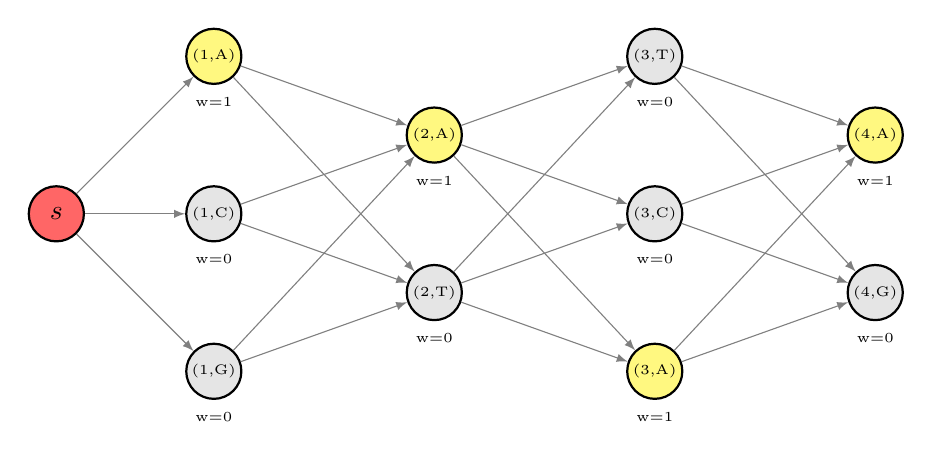
\begin{tikzpicture}[
            node distance=2.8cm and 1.0cm, % x distance and y distance
            node_style/.style={circle, draw, thick, minimum size=7mm, inner sep=0pt},
            weight_one/.style={node_style, fill=yellow!50},
            weight_zero/.style={node_style, fill=gray!20},
            source_node/.style={node_style, fill=red!60},
            edge_style/.style={->, >=latex, thin, gray},
            level_label/.style={font=\footnotesize, below=12mm of #1}
        ]

        % Nodes arranged by level (k) vertically aligned
        \node[source_node] (s) at (0, 0) {$s$};

        % Vertices for k=1 (X1 = {A, C, G})
        \node[weight_one] (v1A) at (2, 2) {\tiny (1,A)}; \node[below=1pt of v1A] {\tiny w=1};
        \node[weight_zero](v1C) at (2, 0) {\tiny (1,C)}; \node[below=1pt of v1C] {\tiny w=0};
        \node[weight_zero](v1G) at (2,-2) {\tiny (1,G)}; \node[below=1pt of v1G] {\tiny w=0};
        % \node[level_label=v1C] (l1) {$k=1$}; % Label for level 1

        % Vertices for k=2 (X2 = {A, T})
        \node[weight_one] (v2A) at (4.8, 1) {\tiny (2,A)}; \node[below=1pt of v2A] {\tiny w=1};
        \node[weight_zero](v2T) at (4.8,-1) {\tiny (2,T)}; \node[below=1pt of v2T] {\tiny w=0};
        % \node[level_label=v2A] (l2) {$k=2$}; % Label for level 2

        % Vertices for k=3 (X3 = {T, C, A})
        \node[weight_zero] (v3A) at (7.6, 2) {\tiny (3,T)}; \node[below=1pt of v3A] {\tiny w=0};
        \node[weight_zero](v3C) at (7.6, 0) {\tiny (3,C)}; \node[below=1pt of v3C] {\tiny w=0};
        \node[weight_one](v3T) at (7.6,-2) {\tiny (3,A)}; \node[below=1pt of v3T] {\tiny w=1};
        % \node[level_label=v3C] (l3) {$k=3$}; % Label for level 3

        % Vertices for k=4 (X4 = {A, G})
        \node[weight_one] (v4A) at (10.4, 1) {\tiny (4,A)}; \node[below=1pt of v4A] {\tiny w=1};
        \node[weight_zero](v4G) at (10.4,-1) {\tiny (4,G)}; \node[below=1pt of v4G] {\tiny w=0};
        % \node[level_label=v4A] (l4) {$k=4$}; % Label for level 4

        % Edges
        % s to Level 1
        \foreach \v in {v1A, v1C, v1G} { \draw[edge_style] (s) -- (\v); }

        % Level 1 to Level 2 (All-to-all)
        \foreach \u in {v1A, v1C, v1G} {
                \foreach \v in {v2A, v2T} {
                        \draw[edge_style] (\u) -- (\v);
                    }
            }

        % Level 2 to Level 3 (All-to-all)
        \foreach \u in {v2A, v2T} {
                \foreach \v in {v3A, v3C, v3T} {
                        \draw[edge_style] (\u) -- (\v);
                    }
            }

        % Level 3 to Level 4 (All-to-all)
        \foreach \u in {v3A, v3C, v3T} {
                \foreach \v in {v4A, v4G} {
                        \draw[edge_style] (\u) -- (\v);
                    }
            }

    \end{tikzpicture}
    \caption{The weighted DAG $G_A$ derived from the degenerate string in Figure \ref{fig:degenerate_example_tabular_v3} for character $c=\emph{A}$. Nodes visually labeled $(k,a)$ represent the vertices $v_{k,a}$. Nodes with $w_A(v_{k,a})=1$ are yellow; those with $w_A(v_{k,a})=0$ are gray. Edges represent the connections defined in $E_A$.}
    \label{fig:degenerate_dag_horizontal_v3}
\end{figure}

This graph-based perspective on degenerate strings serves as a concrete starting point for the core topic of this chapter: the development of succinct data structures for general node-weighted DAGs to support path-based queries. We address the challenge of representing an arbitrary DAG $G=(V, E, w)$, where each vertex $v \in V$ carries a non-negative integer weight $w(v)$, in a compressed format that efficiently supports queries related to cumulative path weights. Such weighted DAGs model various phenomena beyond degenerate strings. For example, in bioinformatics, pangenome graphs\footnote{Pangenome graphs may contain cycles. These cycles can be addressed by either removing them or by utilizing path information provided by modern pangenome graph formats.} can be interpreted through this lens: if each node corresponds to a DNA sequence (a string over $\{A, C, G, T\}$), the weight $w(v)$ could represent the count of a specific nucleotide (e.g., \emph{A}) within that sequence; similarly for \emph{C}, \emph{G}, and \emph{T}.

Our primary focus is on generalizing the \Rank{} query to this graph setting; the \textsf{select} query, while definable, will not be treated further in this work. For a given vertex $N$, the \textsf{rank} query aims to describe the set of possible cumulative weights achievable on paths originating from a designated source vertex $s$ and terminating at $N$.

The combinatorial complexity of paths in a DAG - potentially exponential in the number of vertices - makes naive approaches based on explicit path enumeration or storage infeasible for large graphs. This motivated us to development of a \emph{succinct} data structure. Our approach involves partitioning the vertices based on how their path weight information is represented: some vertices (\emph{explicit}) will store this information directly, while others (\emph{implicit}) will rely on indirect derivation through references facilitated by a carefully defined \emph{successor} relationship, as detailed in Section \ref{sec:succinct_dag_representation}.


% \section{Rank \& Select}

% Let's start by addressing the following problem: consider a dictionary $\mathcal{D}$ of $n$ strings drawn from an alphabet $\Sigma$. We can represent the whole dictionary as a single string $T[1,m]$\footnote{Without any separator between strings} by concatenating all the strings in $\mathcal{D}$, where $m$ is the total length of the dictionary. The problem is to support the following queries:
% \begin{itemize}
%     \item \texttt{Access\_string(i)}: return the $i$-th string in $\mathcal{D}$.
%     \item \texttt{Which\_string(x)}: retrieve the starting position of the string in $T$ including
%     the symbol $T[x]$.
% \end{itemize}
% The classic approach to solve this problem is via an array of pointers A[1, n] to $\mathcal{D}$'s strings, implemented by means of their offsets in $T[1, m]$, thus using $\theta(n \log n)$ bits overall. So the operation \texttt{Access\_string(i)} boils down to returning $A[i]$, whereas \texttt{Which\_string(x)} boils down to finding the predecessor of $x$ in $A$. The first operation takes constant time, while the second one takes $O(\log n)$ time via binary search.

In the previous chapter, we introduced various methods for compressing data. Now we introduce the concept of compressed data structures: data structures that store data in a compressed form, allowing for efficient access to the data. This will lead to the introduction of the so called \emph{pointer-less programming}, where we ditch the traditional pointers and instead use compressed data structures built upon binary arrays that allow for efficient access to the data. In this chapter, we will introduce the concept of bitvectors, and show how they can be compressed to support rank and select queries in constant time. We will then introduce wavelet trees, a data structure that generalizes the concept of bitvectors to support rank and select queries on arbitrary alphabets. \\

TODO: Change this introduction, I don't like it

\section{Bitvectors} \label{sec:bitvectors}
Consider the following problem \cite{ferragina2023pearls}: imagine a dictionary $\mathcal{D}$ containing $n$ strings from an alphabet $\Sigma$. We can merge all strings in $\mathcal{D}$ into a single string $T[1,m]$, without any separators between them, where $m$ is the total length of the dictionary. The task is to handle the following queries:
\begin{itemize}
    \item \texttt{Read(i)}: retrieve the $i$-th string in $\mathcal{D}$.
    \item \texttt{Which\_string(x)}: find the starting position of the string in $T$, including the character $T[x]$.
\end{itemize}
The conventional solution involves employing an array of pointers $A[1, n]$ to the strings in $\mathcal{D}$, represented by their offsets in $T[1, m]$, requiring $\Theta(n \log n)$ bits. Consequently, \texttt{Read(i)} simply returns $A[i]$, while \texttt{Which\_string(x)} involves locating the predecessor of $x$ in $A$. The first operation is instantaneous, whereas the second one necessitates $O(\log n)$ time using binary search. \vspace{0.4cm}

\noindent We can address the problem by employing a compressed representation of the offsets in $A$ via a binary array $B[1,m]$ of $m$ bits, where $B[i] = 1$ if and only if $i$ is the starting position of a string in $T$. In this case then $\texttt{Access\_string(i)}$ searches for the $i$-th $1$ in $B$, while $\texttt{Which\_string(x)}$ counts the number of $1$s in the prefix $B[1,x]$. \vspace{0.4cm}

\noindent In modern literature this two operations are well known as \textit{rank} and \textit{select} queries, respectively.
\begin{definition}[Rank and Select]\label{def:rankselect}
    Given $B[1,n]$ a binary array of $n$ bits (a bitvector), we define the following operations:
    \begin{itemize}
        \item The \textbf{rank} of an index $i$ in $B$ relative to a bit $b$ is the number of occurrences of $b$ in the prefix $B[1,i]$. We denote it as $rank_1(i) = \sum_{j=1}^{i} B[j]$. Similarly we can compute $rank_0(i) = i - rank_1(i)$ in constant time.
        \item The \textbf{select} of the $i$-th occurrence of a bit $b$ in $B$ is the index of the $i$-th occurrence of $b$ in $B$. We denote it as $select_b(i)$. Opposite to rank, we can't derive select of $0$ from select of $1$ in constant time.
    \end{itemize}
\end{definition}
\begin{example}
    TODO: Maybe add a simple example of a bitvector and show how to compute rank and select.
\end{example}
% \noindent In the following sections, our aim is to compress bitvectors to $n \mathcal{H}_k(B) + o(n)$ bits, where $\mathcal{H}_k(B)$ denotes the $k$-th order empirical entropy of $B$. The pivotal strategy for achieving compression lies in encoding bit blocks as a single unit. Following this, we will construct structures of size $o(n)$ bits that can be added on top either the bit array or the compressed representation of $B$ to facilitate rank and select operations.
\noindent As stated before, bitvectors are the fundamental piece in the implementation of compressed data structures. Therefore, an efficient implementation is crucial. In the following sections, our aim is to built structures of size $o(n)$ bits that can be added on top either the bit array or the compressed representation of $B$ to facilitate rank and select operations. We will see that will often encounter skewed distributions of $0$s and $1$s in $B$, and we will exploit this property to achieve higher order compression.

\begin{remark}
    If we try to compress bitvectors with the techniques seen in \autoref{ch:Chapter2}, we would need to encode each bit individually, requiring at least
\end{remark}

\noindent TBD: Do I talk also about how to compress the bitvector to $n \mathcal{H}_0(B) + o(n)$ bits with those extra $o(n)$ to support rank and select operations still in $O(1)$ time? There is also the compressed solution via Elias Fano, when the numbers of $1s$ in B is much smaller than $n$, where I can achieve $n\mathcal{H}_0(B) + O(m)$ bits of space occupancy. This approach poses a much lower overhead over the entropy. It supports $Select$ in constant time, while $access$ and $Rank$ in $O(\log \frac{n}{m})$ \cite{navarro2016compact,ferragina2023pearls}. On a further note, in \cite{FERRAGINA2007115} Ferragina and Venturini achieved higher order compression for general strings, supporting access in constant time (so adding rank and select for bitvectors are natural extensions), do I talk about this as well?

\subsection{Rank}

In their seminal paper \cite{RRR2002} Raman et al. introduced a hierarchical succinct data structure that supports the rank operation in constant time, while only using $n + o(n)$ bits of space. The structure is based on the idea of splitting the binary array $B[1, n]$ into big and small blocks of fixed length, and then encoding the number of bits set to $1$ in each block. \vspace{0.4cm}

\noindent More precisely, the structure is composed of three levels: in the first one we (logically) split $B[1, n]$ into blocks of size $Z$ each, where at the beginning of each superblock we store the number of bits set to $1$ in the corresponding block, i.e the output of the query $rank_1(i)$ for $i$ being the starting position of the block. In the second level, we split the superblocks into blocks of size $z$ bits each\footnote{For simplicty, we assume that $z$ divides $Z$} with the same meta-information stored at the beginning of each block. Finally the third level is a lookup table that indexed by the small blocks and queried positions. In other words, for each possible small block and each possible position within that block, the lookup table stores the result of the $rank_1$ operation. This pre-computed information allows for constant time retrieval of the $rank_1$ operation results, as the result can be directly looked up in the table instead of having to be computed each time. This is the key to the efficiency of the data structure. In this way, the $i-th$ block, of size $Z$, can be accessed as
\[
    B[i \cdot Z + 1, (i+1) \cdot Z]
\]
while the small block $j$ of size $z$ in the $i-th$ superblock is
\[
    B[i \cdot Z + j \cdot z + 1, i \cdot Z + (j+1) \cdot z] \qquad \forall j \in [0, Z/z), \forall i \in [0, n/Z)
\]
We will denote with $r_i$ the number of bits set to $1$ in the $i-th$ block, and with $r_{i,j}$ the number of bits set to $1$ in the $j-th$ small block of the $i-th$ superblock. Figure \ref{fig:RRR} shows a visual representation of the RRR data structure.

\begin{figure}[h]
    \begin{flushright}
        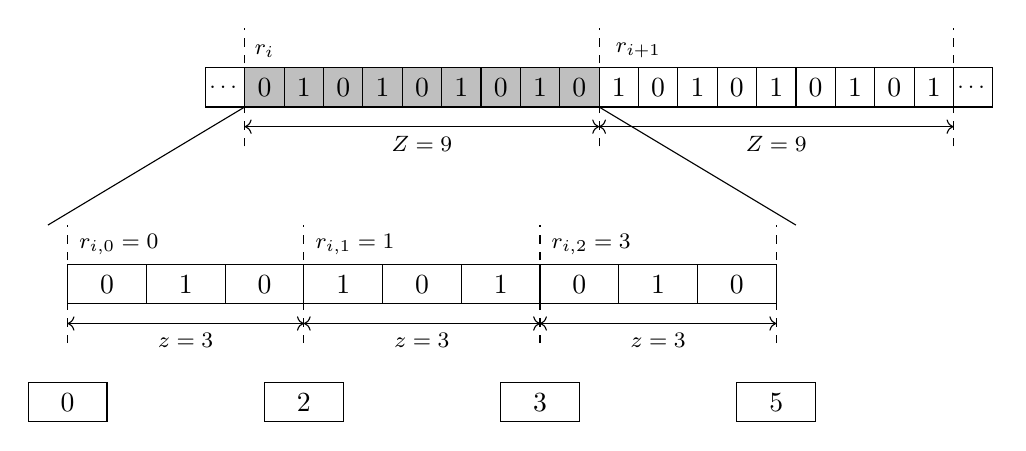
\begin{tikzpicture}[scale=0.5] % Adjust the scale as needed
            \foreach \x/\bit in {0/\footnotesize{\dots}, 1/0, 2/1, 3/0, 4/1, 5/0, 6/1, 7/0, 8/1, 9/0, 10/1, 11/0, 12/1, 13/0, 14/1, 15/0, 16/1, 17/0, 18/1, 19/\footnotesize{\dots}} {
                    \ifnum\x<1
                        \draw (\x,0) rectangle (\x+1,1) node[midway] {\bit};
                    \else
                        \ifnum\x<10
                            \draw[fill=lightgray] (\x,0) rectangle (\x+1,1) node[midway] {\bit};
                        \else
                            \draw (\x,0) rectangle (\x+1,1) node[midway] {\bit};
                        \fi
                    \fi
                }
            % Add dashed lines
            \draw[dashed] (1,-1) -- (1,2);
            \draw[dashed] (10,-1) -- (10,2);
            \draw[dashed] (19,-1) -- (19,2);

            % add double arrow
            \draw[<->] (1,-0.5) -- (10,-0.5) node[midway, below] {\footnotesize{$Z=9$}};
            \draw[<->] (10,-0.5) -- (19,-0.5) node[midway, below] {\footnotesize{$Z=9$}};

            % Add label over the blocks 2, 10
            \node[above] at (1.5,1) {\footnotesize{$r_i$}};
            \node[above] at (11,1) {\footnotesize{$r_{i+1}$}};

            % Add one line that starts from the bottom angle of block 1, and goes down inclined
            \draw[-] (1,0) -- (-4,-3);
            \draw[-] (10,0) -- (15,-3);

            \foreach \x/\bit in {0/0, 1/1, 2/0, 3/1, 4/0, 5/1, 6/0, 7/1, 8/0} {
                    \draw (\x*2-3.5,-5) rectangle (\x*2-1.5,-4) node[midway] {\bit};
                }

            % Add dashed lines
            \draw[dashed] (-3.5,-6) -- (-3.5,-3);
            \draw[dashed] (2.5,-6) -- (2.5,-3);
            \draw[dashed] (8.5,-6) -- (8.5,-3);
            \draw[dashed] (14.5,-6) -- (14.5,-3);

            % add double arrow
            \draw[<->] (-3.5,-5.5) -- (2.5,-5.5) node[midway, below] {\footnotesize{$z=3$}};
            \draw[<->] (2.5,-5.5) -- (8.5,-5.5) node[midway, below] {\footnotesize{$z=3$}};
            \draw[<->] (8.5,-5.5) -- (14.5,-5.5) node[midway, below] {\footnotesize{$z=3$}};

            % Add label over the blocks 2, 10
            \node[above] at (-2.2,-4) {\footnotesize{$r_{i,0} = 0$}};
            \node[above] at (3.8,-4) {\footnotesize{$r_{i,1} = 1$}};
            \node[above] at (9.8,-4) {\footnotesize{$r_{i,2} = 3$}};

            % Under the first block, add a block of the same size with 0 inside. Under the 4th block, add a block of the same size with 2 inside. Under the 7th block, add a block of the same size with 3 inside. Under the 10th block, add a block of the same size with 5 inside.

            \foreach \x/\bit in {-4.5/0, 1.5/2, 7.5/3, 13.5/5} {
                    \draw (\x,-8) rectangle (\x+2,-7) node[midway] {\bit};
                }

        \end{tikzpicture}
    \end{flushright}
    \caption{The RRR Rank data structure}
\end{figure}

% TODO:
% \begin{itemize}
%     \item Explain the tree level succinct data structure supporting the rank operation as in RRR \cite{RRR2002}
%     \item Proof of the space occupancy in bits of the structure. \cite{ferragina2023pearls}
%     \item Explain how to answer rank queries upon this data structure \cite{ferragina2023pearls,navarro2016compact}
% \end{itemize}
\begin{theorem}
    The space occupancy of the Rank data structure is $o(m)$ bits, and thus it is asymptotically sublinear in the size of the binary array $B[1, m]$. The Rank algorithm takes constant time in the worst case, and accesses the array $B$ only in read-mode
\end{theorem}
TBD: Do I talk about \cite{grossi2009haste}?
\begin{example}
    TODO: numeric small example to show how to answer rank queries.
\end{example}

\subsection{Select}
TODO:
\begin{itemize}
    \item Explain how to the implementation of the Select operation mainly follows the three-level design of the Rank data structure, with the algorithmic twist that here the binary array $B$ is not split into big and small blocks of fixed length, but the splitting is driven by the number of bits set to $1$. \cite{ferragina2023pearls,navarro2016compact}
    \item Talk about the space occupancy in bits of the structure. \cite{ferragina2023pearls,navarro2016compact}
\end{itemize}

\begin{theorem}
    The space occupancy of the $Select_1$ data structure is $o(m)$ bits, and thus it is asymptotically sublinear in the size of the binary array $B[1, m]$. The $Select_1$ algorithm takes constant time in the worst case, and accesses the array $B$ only in read-mode. The same time and space bounds hold for the $Select_0$ algorithm. \cite{ferragina2023pearls}
\end{theorem}


% \subsection{An Efficient Rank Structure: RRR}
% In this section we will see a static bit sequence data structure that answer rank queries in $O(1)$ time, thus providing implicit compression. This structures is known RRR and was introduced by Raman, Raman and Rao in 2002 \cite{RRR2002} with the purpose


% \subsection{Strings}

% --- SLIDE 7: Beyond Bits: General Alphabets ---
\begin{frame}{Beyond Bitvectors: General Alphabets}
    \framesubtitle{Wavelet Trees}
    \vspace{-0.2em}
    What about sequences $S[1..n]$ over larger alphabets $\Sigma = \{1, \dots, \sigma\}$?
    \begin{figure}[hbtp]
        \centering
        \only<2>{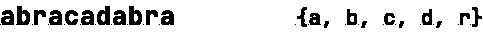
\includegraphics[width=0.6\textwidth]{assets/wt1.pdf}} % Visible only on slide 2
        \only<3>{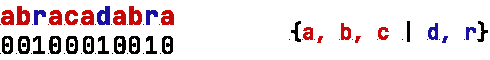
\includegraphics[width=0.7\textwidth]{assets/wt2.pdf}} % Visible only on slide 3
        \only<4>{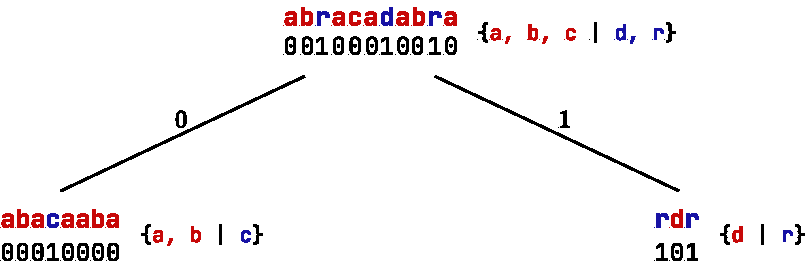
\includegraphics[width=\textwidth]{assets/wt3.pdf}} % Visible only on slide 4
        \only<5>{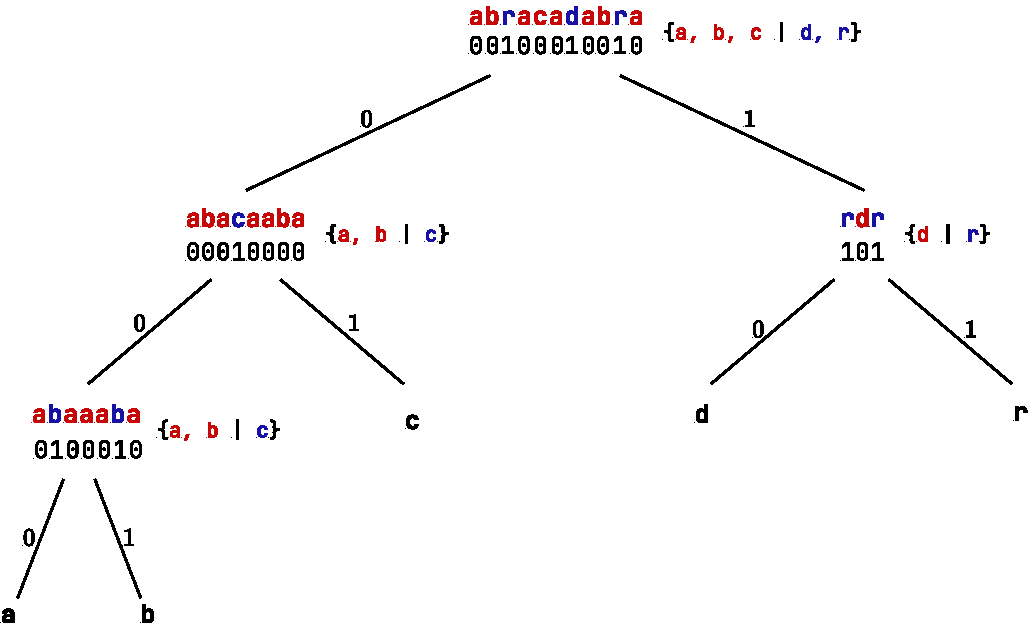
\includegraphics[width=0.7\textwidth]{assets/wt4.pdf}} % Visible ONLY on slide 5
    \end{figure}
    \only<6->{
        \begin{columns}[T] % Align columns at the top
            \begin{column}{0.55\textwidth} % Adjust width as needed
                \centering % Center the image in the column
                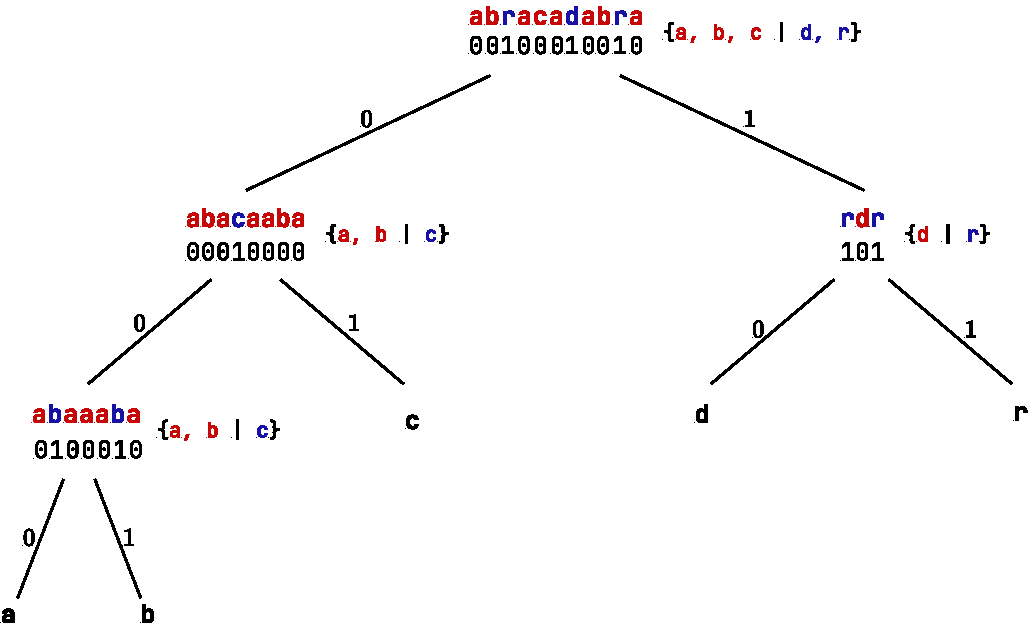
\includegraphics[width=\textwidth]{assets/wt4.pdf} % Show from slide 6 onwards
            \end{column}
            \begin{column}{0.45\textwidth} % Adjust width as needed
                \begin{block}{$\mathcal{H}_0$-Compressed Wavelet Tree} % Ref Thm 3.8 in thesis
                    Using RRR for bitvectors:
                    \begin{itemize}
                        \item \textbf{Space}: $n \mathcal{H}_0(S) + o(n \log \sigma)$ bits.
                        \item \textbf{Query Time}: $O(\log \sigma)$ for \textsf{access}, \textsf{rank}$_c$, \textsf{select}$_c$.
                    \end{itemize}
                    Adapts space to the sequence's zero-order entropy.
                \end{block}
            \end{column}
        \end{columns}
    }
\end{frame}

% \begin{frame}{Wavelet Tree Construction: Example}
%     \framesubtitle{Step 1: Splitting the Root}
%     \begin{columns}[T,totalwidth=\textwidth] % Colonne allineate in alto
%         % Colonna sinistra: Spiegazioni
%         \begin{column}{0.5\textwidth}
%             % Spazio sopra allineato con l'alfabeto a destra
%             \vspace*{1ex} % Aggiusta se necessario

%             \uncover<1->{
%                 \textbf{1. Alphabet Split:}
%                 \begin{itemize}
%                     \item Root covers $\Sigma = \{\texttt{a, b, c, d, r}\}$.
%                     \item Use range $[1, 5]$.
%                     \item Midpoint $m = 3$ is \alert{c}.
%                     \item Split into: $[\texttt{a, b, c}]$ vs $[\texttt{d, r}]$.
%                 \end{itemize}
%                 \bigskip
%             }
%             \uncover<2->{
%                 \textbf{2. Bitmap Rule ($B_{root}$):}
%                 \begin{itemize}
%                     \item If char $\le$ \alert{c} $\rightarrow$ Bit \textcolor{blue!70!black}{0} (Goes Left)
%                     \item If char $>$ \alert{c} $\rightarrow$ Bit \textcolor{red!70!black}{1} (Goes Right)
%                 \end{itemize}
%                 \bigskip
%             }
%         \end{column}

%         % Colonna destra: Visualizzazione
%         \begin{column}{0.5\textwidth}
%             \centering
%             % Spazio sopra allineato con l'alfabeto a sinistra
%             \vspace*{9ex} % Aggiusta se necessario

%             % Visualizzazione dell'alfabeto
%             \uncover<2->{
\includegraphics[width=0.5\textwidth]{../bachelor-thesis/TeX/assets/WT_slides_root.pdf}} % Mostra solo quando necessario
%         \end{column}
%     \end{columns}
% \end{frame}

% \begin{frame}{Wavelet Tree Construction: Example}
%     \framesubtitle{Building the Tree}
%     \begin{figure}[hbtp]
%         \centering
%         % Replace TikZ with sequential images
%         \only<1>{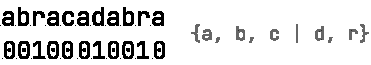
\includegraphics[width=0.7\textwidth]{../bachelor-thesis/TeX/assets/WT_slides1.pdf}} % Visible only on slide 2
%         \only<2>{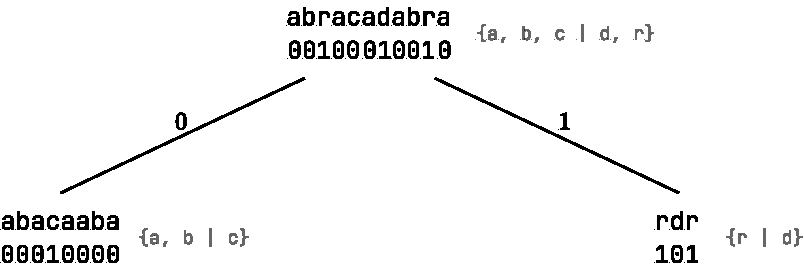
\includegraphics[width=0.7\textwidth]{../bachelor-thesis/TeX/assets/WT_slides2.pdf}} % Visible only on slide 3
%         \only<3->{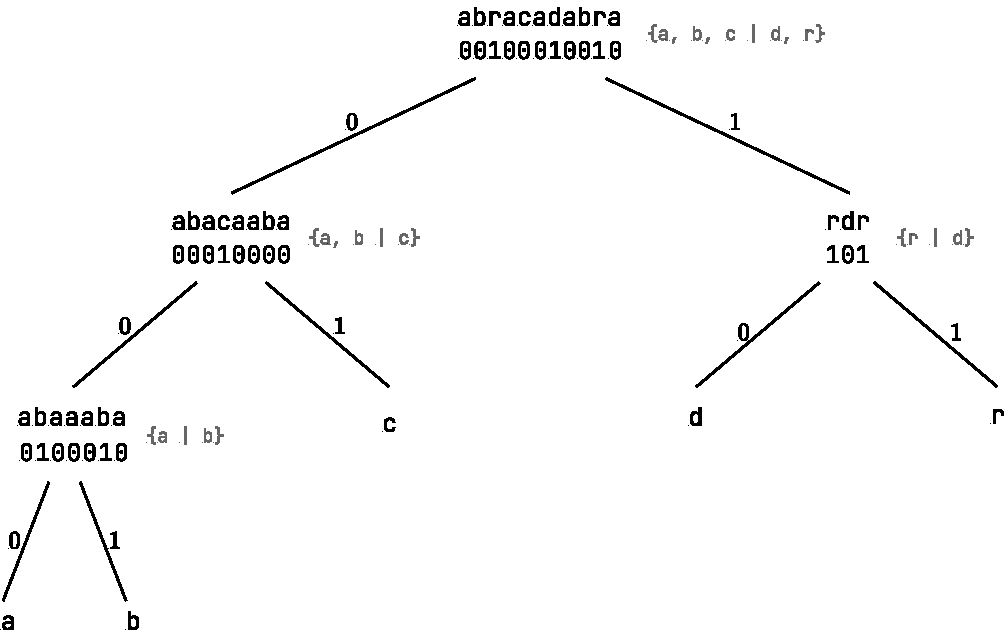
\includegraphics[width=0.7\textwidth]{../bachelor-thesis/TeX/assets/WT_slides3.pdf}} % Visible from slide 4 onwards
%         % \caption{Hierarchical structure for Rank}
%     \end{figure}
% \end{frame}

% \begin{frame}{Wavelet Tree: Rank Example}
%     \framesubtitle{Rank on Wavelet Trees}

%     \begin{figure}[hbtp]
%         \centering
%         % Replace TikZ with sequential images
%         \only<1>{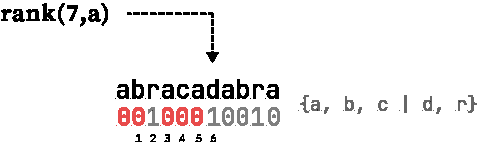
\includegraphics[width=0.7\textwidth]{../bachelor-thesis/TeX/assets/WT_rank_slides1.pdf}} % Visible only on slide 2
%         \only<2>{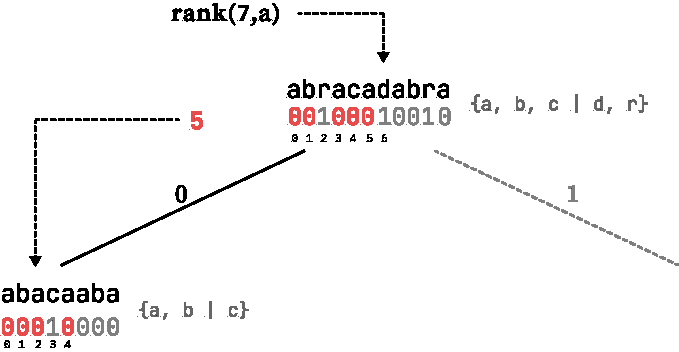
\includegraphics[width=0.7\textwidth]{../bachelor-thesis/TeX/assets/WT_rank_slides2.pdf}} % Visible only on slide 3
%         \only<3->{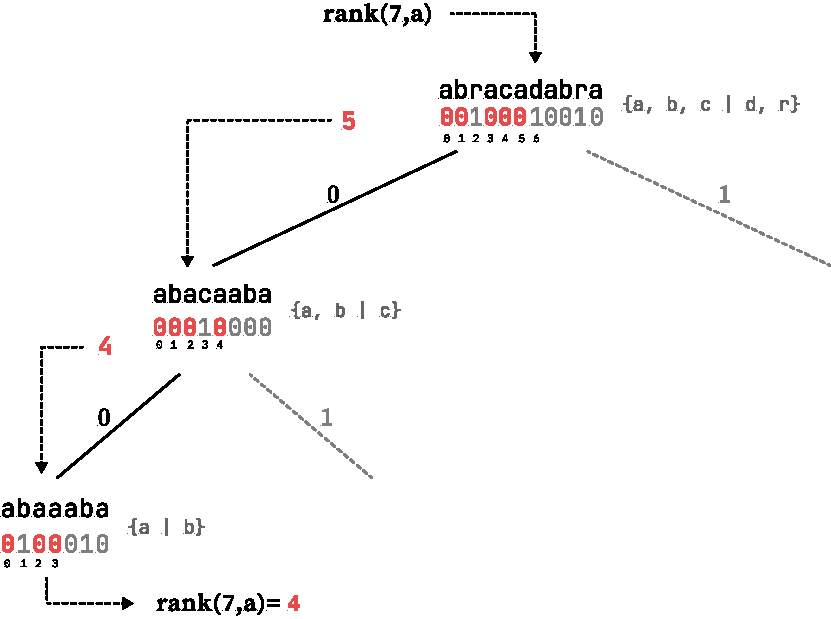
\includegraphics[width=0.65\textwidth]{../bachelor-thesis/TeX/assets/WT_rank_slides3.pdf}} % Visible from slide 4 onwards
%         % \caption{Hierarchical structure for Rank}
%     \end{figure}
% \end{frame}

% % --- SLIDE 8: Wavelet Tree Performance Summary ---
% \begin{frame}{Wavelet Tree: Performance Summary}
%     \framesubtitle{Space and Query Time}

%     % Standard WT Result
%     \begin{theorem}[Standard Wavelet Tree]
%         Represents $S[1..n]$ over $\Sigma=\{1,\dots,\sigma\}$ using:
%         \begin{itemize}
%             \item \textbf{Space}: $n \lceil \log \sigma \rceil + o(n \log \sigma)$ bits.
%             \item \textbf{Query Time}: $O(\log \sigma)$ for \textsf{access}, \textsf{rank}$_c$, \textsf{select}$_c$.
%         \end{itemize}
%     \end{theorem}

%     \pause % Introduce compressed versions

%     % Compressed WT (H0)
%     \begin{theorem}[$\mathcal{H}_0$-Compressed Wavelet Tree] % Ref Thm 3.8 in thesis
%         Using RRR for bitvectors:
%         \begin{itemize}
%             \item \textbf{Space}: $n \mathcal{H}_0(S) + o(n \log \sigma)$ bits.
%             \item \textbf{Query Time}: $O(\log \sigma)$ for \textsf{access}, \textsf{rank}$_c$, \textsf{select}$_c$.
%         \end{itemize}
%         Adapts space to the sequence's zero-order entropy.
%     \end{theorem}
% \end{frame}


% \subsection{Degenerate Strings}

% --- SLIDE 9: Degenerate Strings ---
\begin{frame}{Representing Sequence Variation: Degenerate Strings}
    \framesubtitle{Definitions and Core Operations}
    \begin{block}{Definition and Rank \& Select Adaptation}
        A \textbf{degenerate string} is a sequence $X = X_1 X_2 \dots X_n$, where each $X_i$ is a \emph{subset} of the alphabet $\Sigma$ with cardinality $\sigma$. We can define the following operations:
        \begin{itemize}
            \item \textsf{subset-rank}$_X(i, c)$: Counts sets $X_k$ ($k \le i$) where $c \in X_k$.
            \item \textsf{subset-select}$_X(j, c)$: Finds index $k$ of the $j$-th set $X_k$ where $c \in X_k$.
        \end{itemize}
    \end{block}
    \pause
    \begin{figure}[h!] % Nota: [h!] può essere problematico, [htbp] è più sicuro
        \centering
        \begin{tabular}{c@{\hskip 0.5em}c@{\hskip 0.5em}c@{\hskip 0.5em}c@{\hskip 0.5em}c}
            $X = $                                                               & $\Bigg\{\,\begin{matrix}\texttt{A}\\\texttt{C}\\\texttt{G}\end{matrix}\,\Bigg\}$ &
            $\Bigg\{\,\begin{matrix}\texttt{A}\\\texttt{T}\end{matrix}\,\Bigg\}$ &
            $\Bigg\{\,\begin{matrix}\texttt{C}\end{matrix}\,\Bigg\}$             &
            $\Bigg\{\,\begin{matrix}\texttt{T}\\\texttt{G}\end{matrix}\,\Bigg\}$                                                                                                            \\
                                                                                 & $X_1$                                                                            & $X_2$ & $X_3$ & $X_4$
        \end{tabular}
        \uncover<2->{\qquad
            \begin{tabular}{c@{\hskip 0.5em}c@{\hskip 0.5em}c@{\hskip 0.5em}c@{\hskip 0.5em}c@{\hskip 0.5em}c}
                $S =$  & \texttt{ACG} & \texttt{AT} & \texttt{C} & \texttt{TG} &            \\
                $R = $ & \texttt{100} & \texttt{10} & \texttt{1} & \texttt{10} & \texttt{1} \\
                       & $S_1$        & $S_2$       & $S_3$      & $S_4$
            \end{tabular}
        }
    \end{figure}
    % --- Paragrafo Riscritto ---
    \uncover<3->{% Potrebbe essere utile per far apparire il testo solo al terzo step
        To compute \textsf{subset-rank}$_X(i, c)$: Let $p$ be the end position in $S$ for prefix $X_1..X_i$, found using $\textsf{select}_1(R, i+1)$. The result is $\textsf{rank}_c(S, p)$.
    }
\end{frame}

% % --- SLIDE 10: Degenerate Strings: Space Complexity Results ---
% \begin{frame}{Degenerate Strings: Space Complexity}
%     \framesubtitle{Reduction-Based Approach}

%     % Recall the reduction converts $X$ (length $n$, size $N$) into $S$ (length $N$) and $R$ (length $N+1$).

%     % Blocco 1: Componenti Spazio
%     \begin{block}<1->{Space Components}
%         % The total space depends on:
%         \begin{itemize}
%             \item Storing string $S$: Requires a structure $\mathcal{D}$ supporting \textsf{rank}$_c$/\textsf{select}$_c$.
%             \item Storing bitvector $R$: Requires a structure $\mathcal{V}$ supporting \textsf{rank}/\textsf{select}
%         \end{itemize}
%     \end{block}

%     % Blocco 2: Risultato Generale (Caso n0=0)
%     \begin{block}<2->{Upper Bound (No Empty Sets)}
%         % If $X$ has no empty sets ($n_0 = 0$):
%         \begin{itemize}
%             \item Total Space: $\underbrace{\mathcal{D}_b(N, \sigma)}_{\text{Space for } S} + \underbrace{N + o(N)}_{\text{Space for } R \text{ (succinct)}}$ bits.
%             \item Using standard succinct structures (e.g., Wavelet Tree for $S$, RRR for $R$): Space becomes $\approx N \log \sigma + N + o(N \log \sigma)$ bits.
%         \end{itemize}
%     \end{block}

%     \uncover<3->{\textbf{Lower Bound}: Any structure supporting \texttt{subset-rank} or \texttt{subset-select} requires at least $N \log \sigma - o(N \log \sigma)$ bits in the worst case.}

% \end{frame}


% \section{Path Queries on DAGs}
% \subsection{Path Queries}
% --- SLIDE 11: Connecting Degenerate Strings to DAGs ---
\begin{frame}{From Degenerate Strings to Weighted DAGs}
    \framesubtitle{A New Perspective}

    Recall our degenerate string $X$:
    \begin{figure}[h!]
        \centering
        % Usa la figura della stringa degenere che hai già definito
        \begin{tabular}{c@{\hskip 0.5em}c@{\hskip 0.5em}c@{\hskip 0.5em}c@{\hskip 0.5em}c}
            $X = $                                                                           & $\Bigg\{\,\begin{matrix}\texttt{A}\\\texttt{C}\\\texttt{G}\end{matrix}\,\Bigg\}$ &
            $\Bigg\{\,\begin{matrix}\texttt{A}\\\texttt{T}\end{matrix}\,\Bigg\}$             &
            $\Bigg\{\,\begin{matrix}\texttt{T}\\\texttt{C}\\\texttt{A}\end{matrix}\,\Bigg\}$ &
            $\Bigg\{\,\begin{matrix}\texttt{A}\\\texttt{G}\end{matrix}\,\Bigg\}$                                                                                                                        \\
                                                                                             & $X_1$                                                                            & $X_2$ & $X_3$ & $X_4$
        \end{tabular}
    \end{figure}

    \uncover<2->{
        \begin{block}{Key Idea}
            We can model queries on $X$ by constructing a specific node-weighted Directed Acyclic Graph (DAG) $G_c$ for a target character $c$.
        \end{block}
    }

    \uncover<3->{
        \begin{itemize}
            \item<3-> \textbf{Vertices $V_c$}: Source $s$ + one node $v_{k,a}$ for each character $a \in X_k$ at each position $k$.
            \item<4-> \textbf{Weights $w_c$}: $w_c(s)=0$. $w_c(v_{k,a}) = 1$ if $a = c$, else $0$. (Highlights occurrences of $c$).
            \item<5-> \textbf{Edges $E_c$}: Connect $s$ to $k=1$. Connect all $v_{k,a}$ to all $v_{k+1,b}$. (Represents sequence adjacency).
        \end{itemize}
    }

\end{frame}

% % --- SLIDE 12: Visualizing the DAG Construction (Example: c = A) --- USING \pause
% \begin{frame}{Visualizing the DAG Construction (Example: c = A)}
%     \framesubtitle{Building $G_A$ Step-by-Step}

%     \begin{figure}[h!]
%         \centering
%         \resizebox{\textwidth}{!}{% Resize to fit slide width if needed
%             \begin{tikzpicture}[
%                     node distance=2.8cm and 1.0cm, % x distance and y distance
%                     % Define node styles explicitly for clarity
%                     node_style/.style={circle, draw, thick, minimum size=7mm, inner sep=0pt},
%                     weight_one/.style={node_style, fill=yellow!50},
%                     weight_zero/.style={node_style, fill=gray!20},
%                     source_node/.style={node_style, fill=red!60},
%                     % Edge style
%                     edge_style/.style={->, >=latex, thin, gray}
%                 ]

%                 % --- Step 1: Draw Source Node ---
%                 \node[source_node] (s) at (0, 0) {$s$};

%                 % --- Step 2: Draw Level 1 Nodes and Edges from s ---
%                 \node[weight_one] (v1A) at (2, 2) {\tiny (1,A)}; \node[below=1pt of v1A] {\tiny w=1};
%                 \node[weight_zero](v1C) at (2, 0) {\tiny (1,C)}; \node[below=1pt of v1C] {\tiny w=0};
%                 \node[weight_zero](v1G) at (2,-2) {\tiny (1,G)}; \node[below=1pt of v1G] {\tiny w=0};
%                 \foreach \v in {v1A, v1C, v1G} { \draw[edge_style] (s) -- (\v); }

%                 \pause % Wait for click

%                 % --- Step 3: Draw Level 2 Nodes and Edges from Level 1 ---
%                 \node[weight_one] (v2A) at (4.8, 1) {\tiny (2,A)}; \node[below=1pt of v2A] {\tiny w=1};
%                 \node[weight_zero](v2T) at (4.8,-1) {\tiny (2,T)}; \node[below=1pt of v2T] {\tiny w=0};
%                 \foreach \u in {v1A, v1C, v1G} {
%                         \foreach \v in {v2A, v2T} { \draw[edge_style] (\u) -- (\v); }
%                     }

%                 \pause % Wait for click

%                 % --- Step 4: Draw Level 3 Nodes and Edges from Level 2 ---
%                 \node[weight_zero] (v3T) at (7.6, 2) {\tiny (3,T)}; \node[below=1pt of v3T] {\tiny w=0};
%                 \node[weight_zero](v3C) at (7.6, 0) {\tiny (3,C)}; \node[below=1pt of v3C] {\tiny w=0};
%                 \node[weight_one](v3A) at (7.6,-2) {\tiny (3,A)}; \node[below=1pt of v3A] {\tiny w=1};
%                 \foreach \u in {v2A, v2T} {
%                         \foreach \v in {v3T, v3C, v3A} { \draw[edge_style] (\u) -- (\v); }
%                     }

%                 \pause % Wait for click

%                 % --- Step 5: Draw Level 4 Nodes and Edges from Level 3 ---
%                 \node[weight_one] (v4A) at (10.4, 1) {\tiny (4,A)}; \node[below=1pt of v4A] {\tiny w=1};
%                 \node[weight_zero](v4G) at (10.4,-1) {\tiny (4,G)}; \node[below=1pt of v4G] {\tiny w=0};
%                 \foreach \u in {v3T, v3C, v3A} {
%                         \foreach \v in {v4A, v4G} { \draw[edge_style] (\u) -- (\v); }
%                     }

%             \end{tikzpicture}
%         } % End resizebox
%     \end{figure}

%     % Il testo finale appare dopo l'ultimo pause implicito
%     \begin{center}
%         This connection motivates the core topic: \\ \textbf{Efficient data structures for path-based queries on general node-weighted DAGs.}
%     \end{center}

% \end{frame}


% \begin{frame}{Mathematical Framework: Weighted DAGs}
%     \framesubtitle{Basic Definitions}
%     Given a path $P=(v_0=s, \dots, v_k=v)$ we define $W(P) = \sum_{j=1}^{k} w(v_j)$ as the cumulative weight of the path $P$.
%     % \begin{block}{Path and Path Weight}
%     %     \begin{itemize}
%     %         \item Path $P = (v_0=s, \dots, v_k=v)$.
%     %         \item Weight $W(P) = \sum_{j=1}^{k} w(v_j)$.
%     %     \end{itemize}
%     % \end{block}
%     \begin{figure}[h!]
%         \centering
%         \resizebox{0.95\textwidth}{!}{% Scale to fit column
%             \begin{tikzpicture}[
%                 node distance=1.5cm and 1cm,
%                 base_node/.style={circle, draw=black, thick, minimum size=8mm, inner sep=0pt, font=\sffamily},
%                 root_node/.style={base_node, fill=red!60, text=black},
%                 edge_style/.style={->, >={Stealth[length=2mm]}, thick, draw=black}
%                 ]
%                 % Nodes showing only their weight w(v)
%                 \node[root_node] (0) at (0, 2) {0};
%                 \node[base_node] (1) at (1.5, 0) {1};
%                 \node[base_node] (3) at (1.5, 4) {3};
%                 \node[base_node] (6) at (3.5, 1.5) {6};
%                 \node[base_node] (7) at (4.5, 0) {7};
%                 \node[base_node] (2) at (5.5, 4) {2};
%                 \node[base_node] (9) at (6.5, 2) {9};
%                 \node[base_node] (5) at (9, 0.5) {5};
%                 \node[base_node] (10) at (8.5, 5) {10};
%                 \node[base_node] (8) at (11, 3) {8};

%                 % Edges (same as before)
%                 \draw [edge_style] (0) -- (1); \draw [edge_style] (0) -- (3);
%                 \draw [edge_style] (1) -- (6); \draw [edge_style] (1) -- (7);
%                 \draw [edge_style] (3) -- (2); \draw [edge_style] (3) -- (6);
%                 \draw [edge_style] (6) -- (2); \draw [edge_style] (6) -- (9);
%                 \draw [edge_style] (7) -- (5); \draw [edge_style] (7) -- (9);
%                 \draw [edge_style] (2) -- (10);
%                 \draw [edge_style] (9) -- (5); \draw [edge_style] (9) -- (8);
%                 \draw [edge_style] (10) -- (8); \draw [edge_style] (5) -- (8);
%             \end{tikzpicture}
%         } % End resizebox
%     \end{figure}

%     % \begin{columns}[T]
%     %     % Colonna sinistra: Definizioni
%     %     \begin{column}{0.5\textwidth}
%     %         \begin{block}{Weighted DAG $G=(V, E, w)$}
%     %             \begin{itemize}
%     %                 \item $V$: Finite set of vertices.
%     %                 \item $E$: Directed edges, no cycles.
%     %                 \item $w: V \to \mathbb{N}_0$: Non-negative node weights.
%     %                 \item Unique source $s$ with $w(s)=0$.
%     %             \end{itemize}
%     %         \end{block}
%     %         \begin{block}{Path and Path Weight}
%     %             \begin{itemize}
%     %                 \item Path $P = (v_0=s, \dots, v_k=v)$.
%     %                 \item Weight $W(P) = \sum_{j=1}^{k} w(v_j)$.
%     %             \end{itemize}
%     %         \end{block}
%     %     \end{column}

%     %     % Colonna destra: Figura Esempio DAG (solo pesi)
%     %     \begin{column}{0.5\textwidth}
%     %         \begin{figure}[h!]
%     %             \centering
%     %             \resizebox{0.95\textwidth}{!}{% Scale to fit column
%     %                 \begin{tikzpicture}[
%     %                     node distance=1.5cm and 1cm,
%     %                     base_node/.style={circle, draw=black, thick, minimum size=8mm, inner sep=0pt, font=\sffamily},
%     %                     root_node/.style={base_node, fill=red!60, text=black},
%     %                     edge_style/.style={->, >={Stealth[length=2mm]}, thick, draw=black}
%     %                     ]
%     %                     % Nodes showing only their weight w(v)
%     %                     \node[root_node] (0) at (0, 2) {0};
%     %                     \node[base_node] (1) at (1.5, 0) {1};
%     %                     \node[base_node] (3) at (1.5, 4) {3};
%     %                     \node[base_node] (6) at (3.5, 1.5) {6};
%     %                     \node[base_node] (7) at (4.5, 0) {7};
%     %                     \node[base_node] (2) at (5.5, 4) {2};
%     %                     \node[base_node] (9) at (6.5, 2) {9};
%     %                     \node[base_node] (5) at (9, 0.5) {5};
%     %                     \node[base_node] (10) at (8.5, 5) {10};
%     %                     \node[base_node] (8) at (11, 3) {8};

%     %                     % Edges (same as before)
%     %                     \draw [edge_style] (0) -- (1); \draw [edge_style] (0) -- (3);
%     %                     \draw [edge_style] (1) -- (6); \draw [edge_style] (1) -- (7);
%     %                     \draw [edge_style] (3) -- (2); \draw [edge_style] (3) -- (6);
%     %                     \draw [edge_style] (6) -- (2); \draw [edge_style] (6) -- (9);
%     %                     \draw [edge_style] (7) -- (5); \draw [edge_style] (7) -- (9);
%     %                     \draw [edge_style] (2) -- (10);
%     %                     \draw [edge_style] (9) -- (5); \draw [edge_style] (9) -- (8);
%     %                     \draw [edge_style] (10) -- (8); \draw [edge_style] (5) -- (8);
%     %                 \end{tikzpicture}
%     %             } % End resizebox
%     %         \end{figure}
%     %     \end{column}
%     % \end{columns}
% \end{frame}

% --- SLIDE 13: Path Weight Aggregation: The O-Set Definition ---
\begin{frame}{Path Weight Aggregation: The $\mathcal{O}$-Set}
    \framesubtitle{Capturing All Path Weights}
    Given a path $P=(v_0=s, \dots, v_k=v)$ we define $W(P) = \sum_{j=1}^{k} w(v_j)$
    \begin{alertblock}{Goal}
        Characterize the set of \alert{all possible distinct} cumulative path weights arriving at each node.
    \end{alertblock}
    % \vspace{1em}
    \pause
    \begin{block}{$\mathcal{O}$-Set Definition (Recursive)}
        \begin{itemize}
            \item \textbf{Base Case (Source):} $\mathcal{O}_s = \{0\}$
            \item \textbf{Recursive Step ($v \neq s$):}
                  \[ \mathcal{O}_v = \bigcup_{u \in Pred(v)} \{ y + w(v) \mid y \in \mathcal{O}_u \} = \{ W(P) \mid P \in Path(s, v) \}  \]
                  Keep only \alert{distinct} values. Store as a sorted sequence.
        \end{itemize}
    \end{block}
    % The set $\mathcal{O}_v$ contains \emph{exactly} the weights $W(P)$ for all paths $P$ from source $s$ to $v$.
    % \[ \mathcal{O}_v = \{ W(P) \mid P \in Path(s, v) \} \]

\end{frame}

% --- SLIDE 14: O-Set Construction Example ---
\begin{frame}{$\mathcal{O}$-Set Construction Example}
    \framesubtitle{Visualizing the Recursive Definition}
    \vspace{-0.5em}
    \begin{figure}[hbtp]
        % \centering
        % Replace TikZ with sequential images
        \only<1>{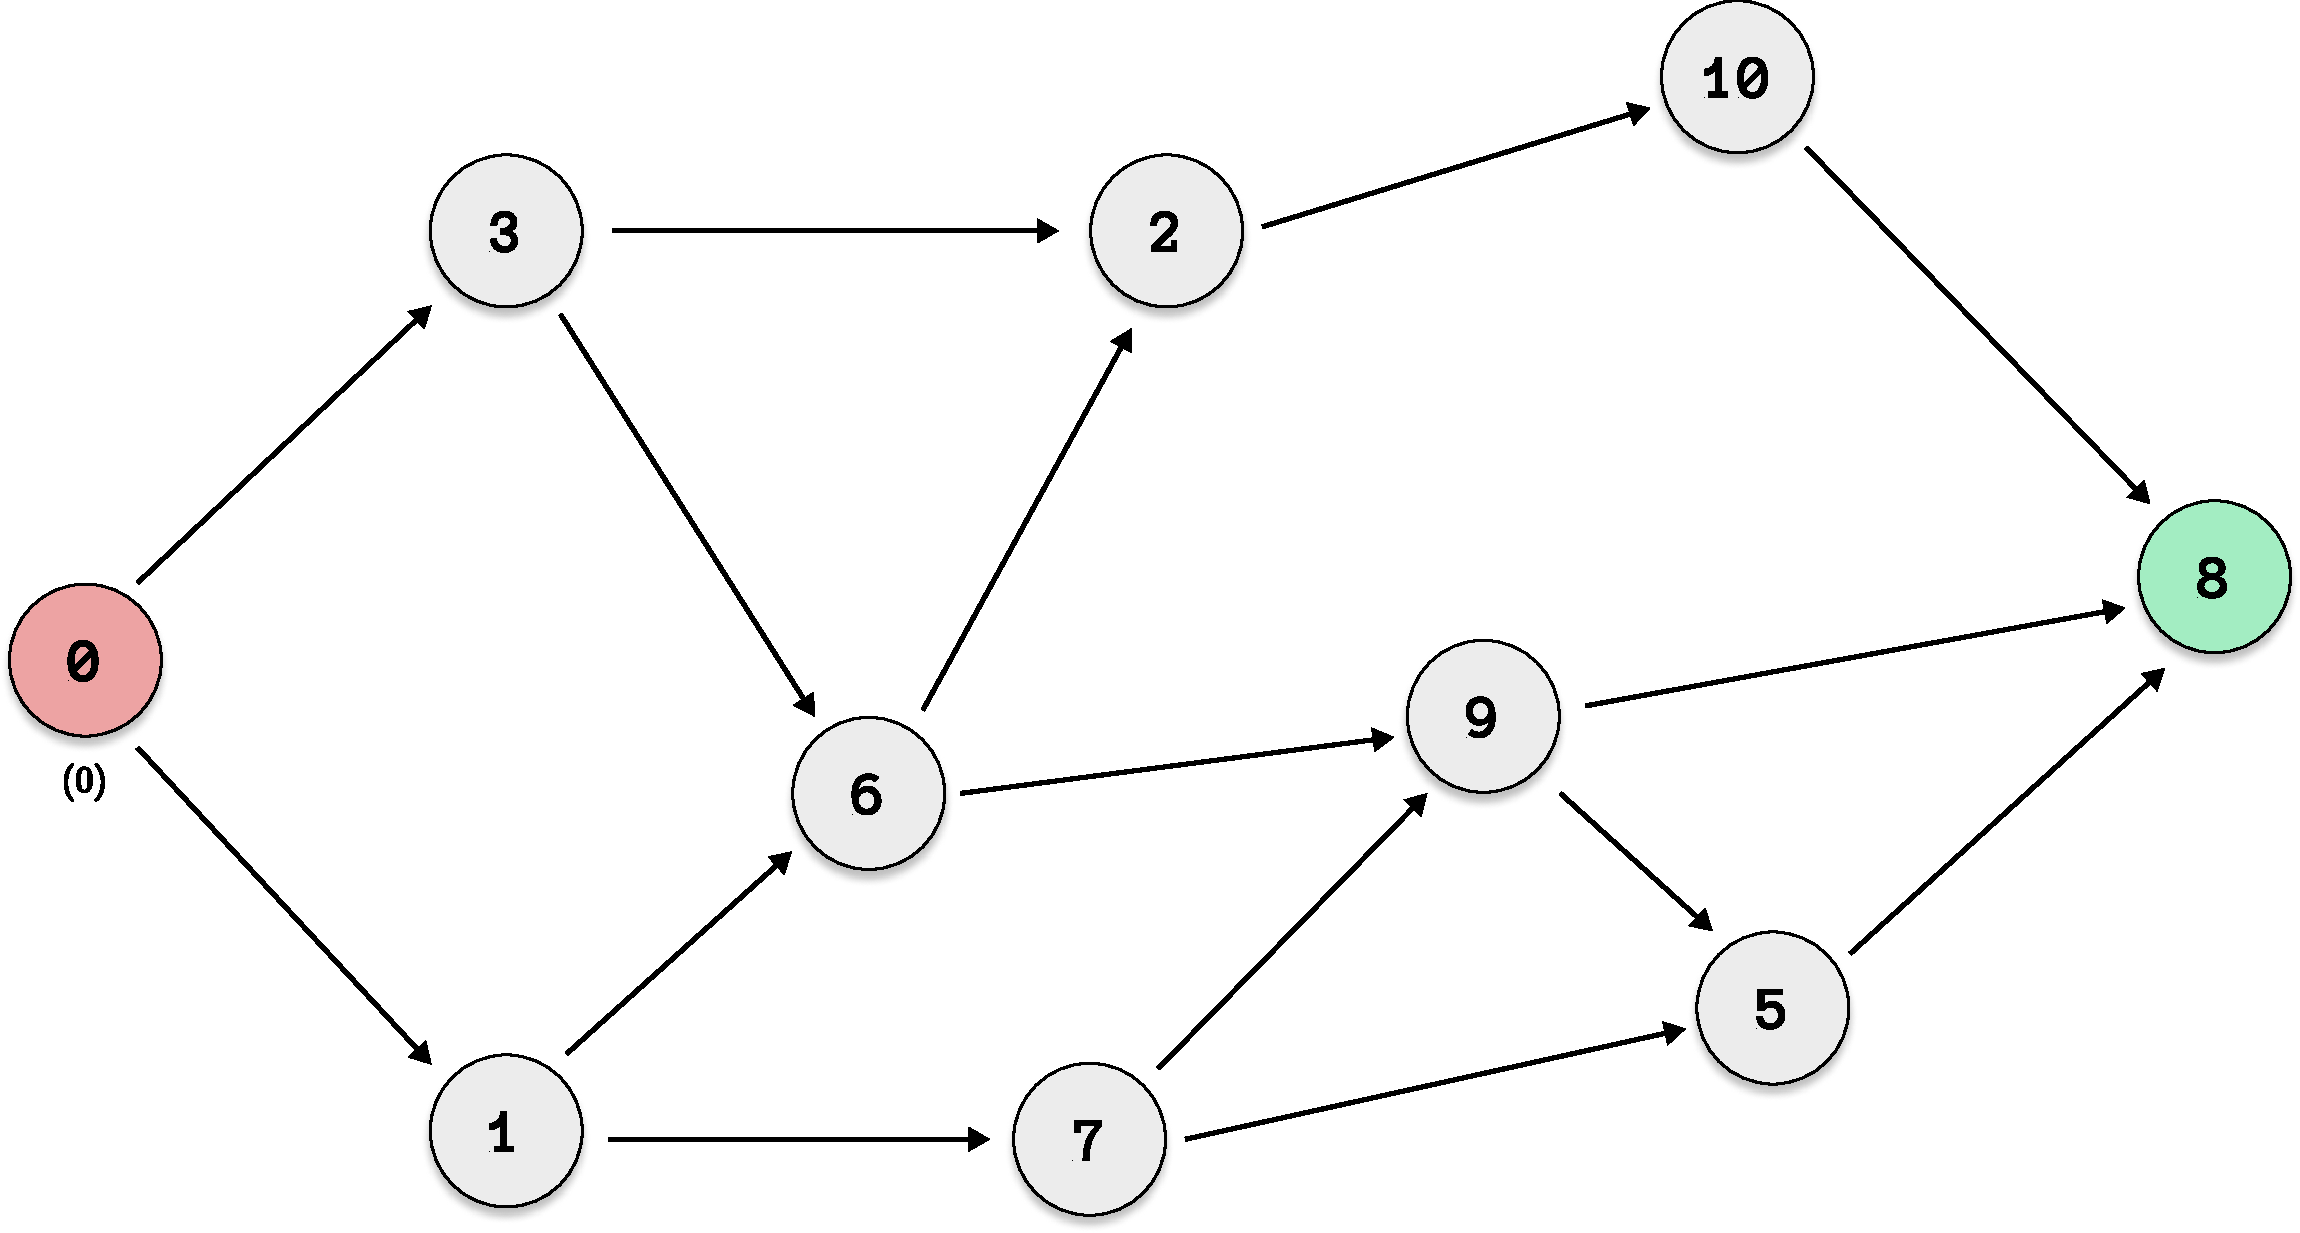
\includegraphics[width=0.9\textwidth]{assets/dag_explicit1.pdf}}
        \only<2>{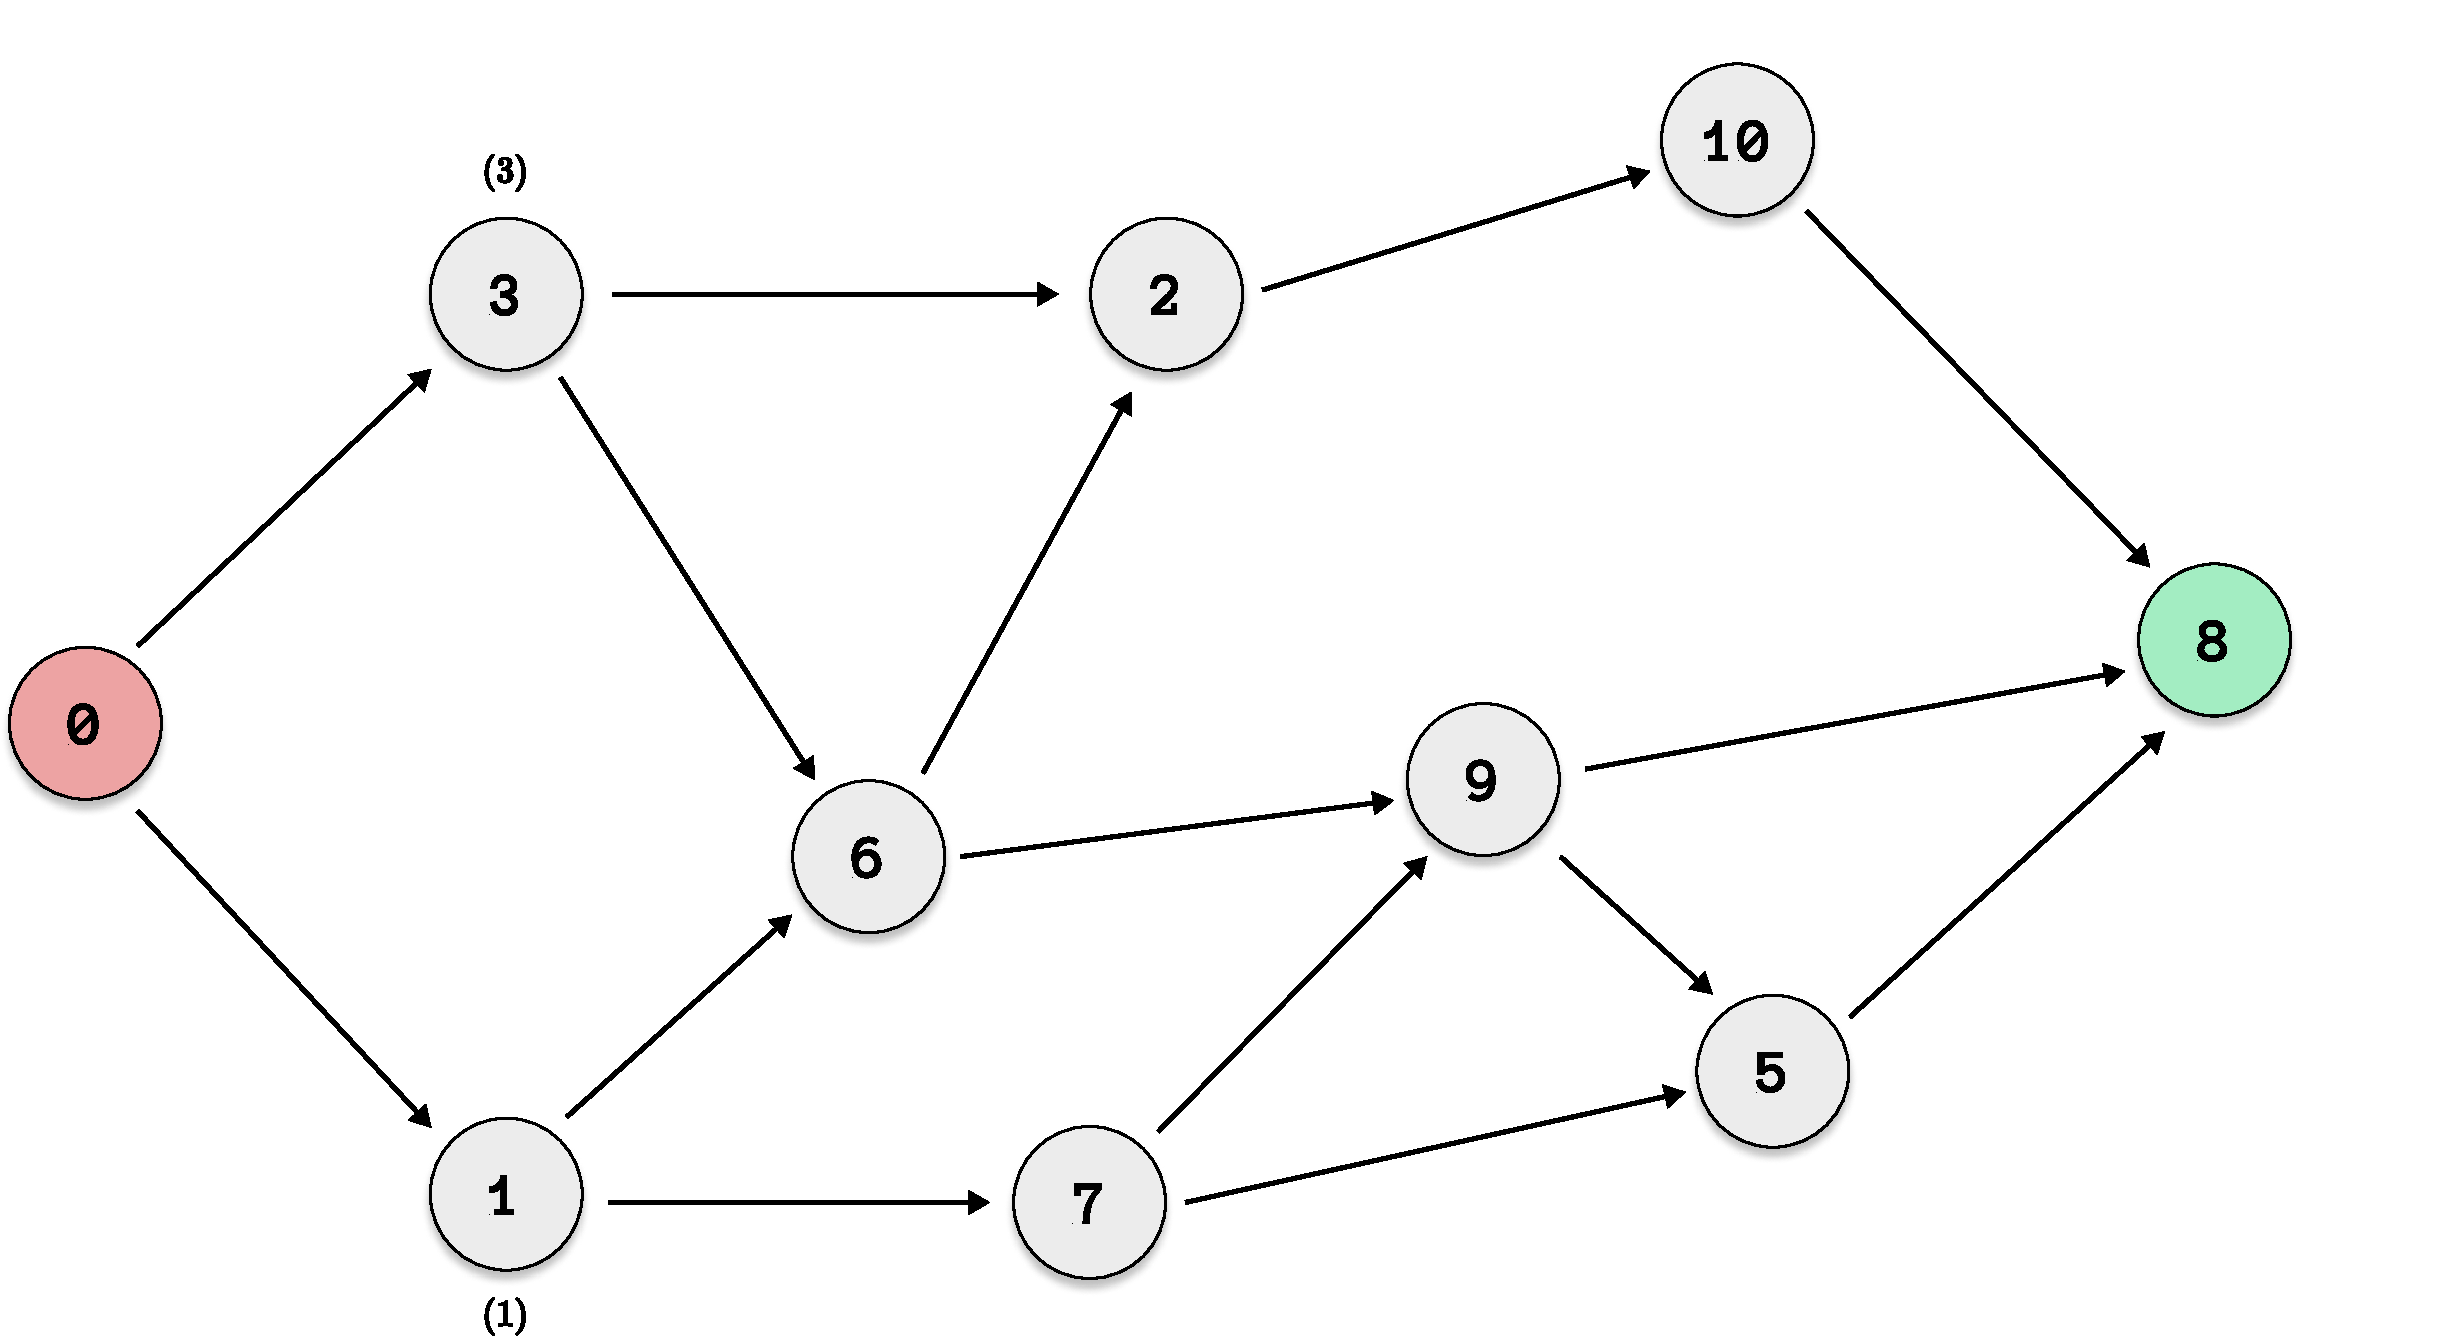
\includegraphics[width=0.9\textwidth]{assets/dag_explicit2.pdf}}
        \only<3>{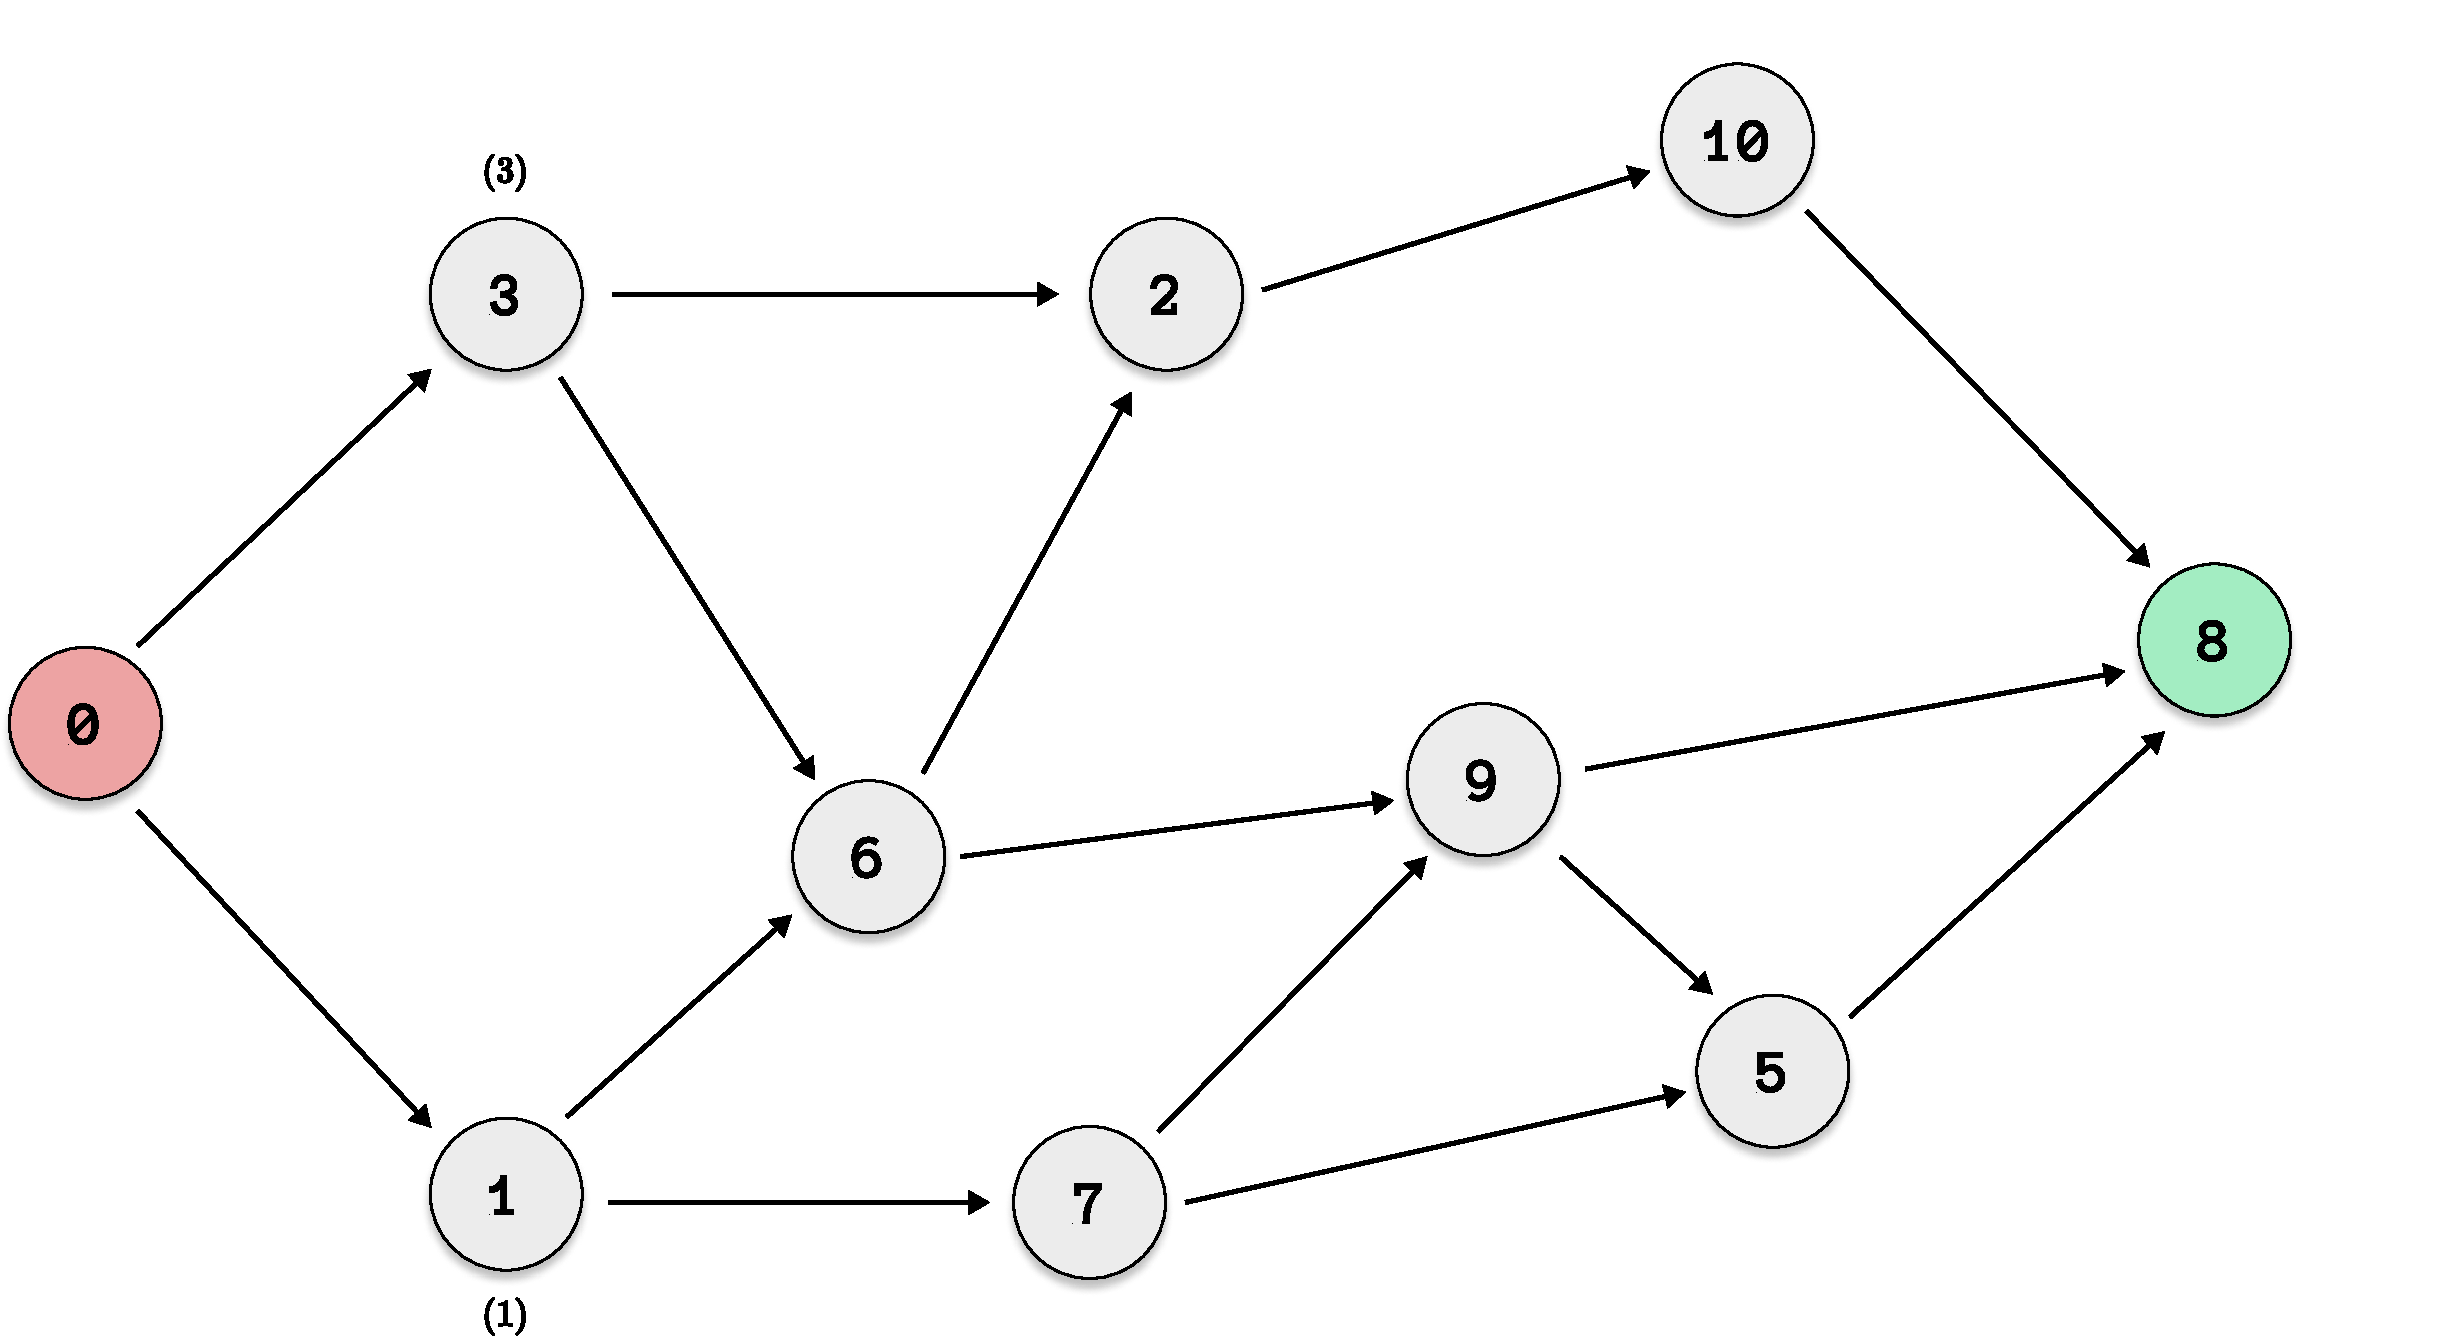
\includegraphics[width=0.9\textwidth]{assets/dag_explicit3.pdf}}
        \only<4>{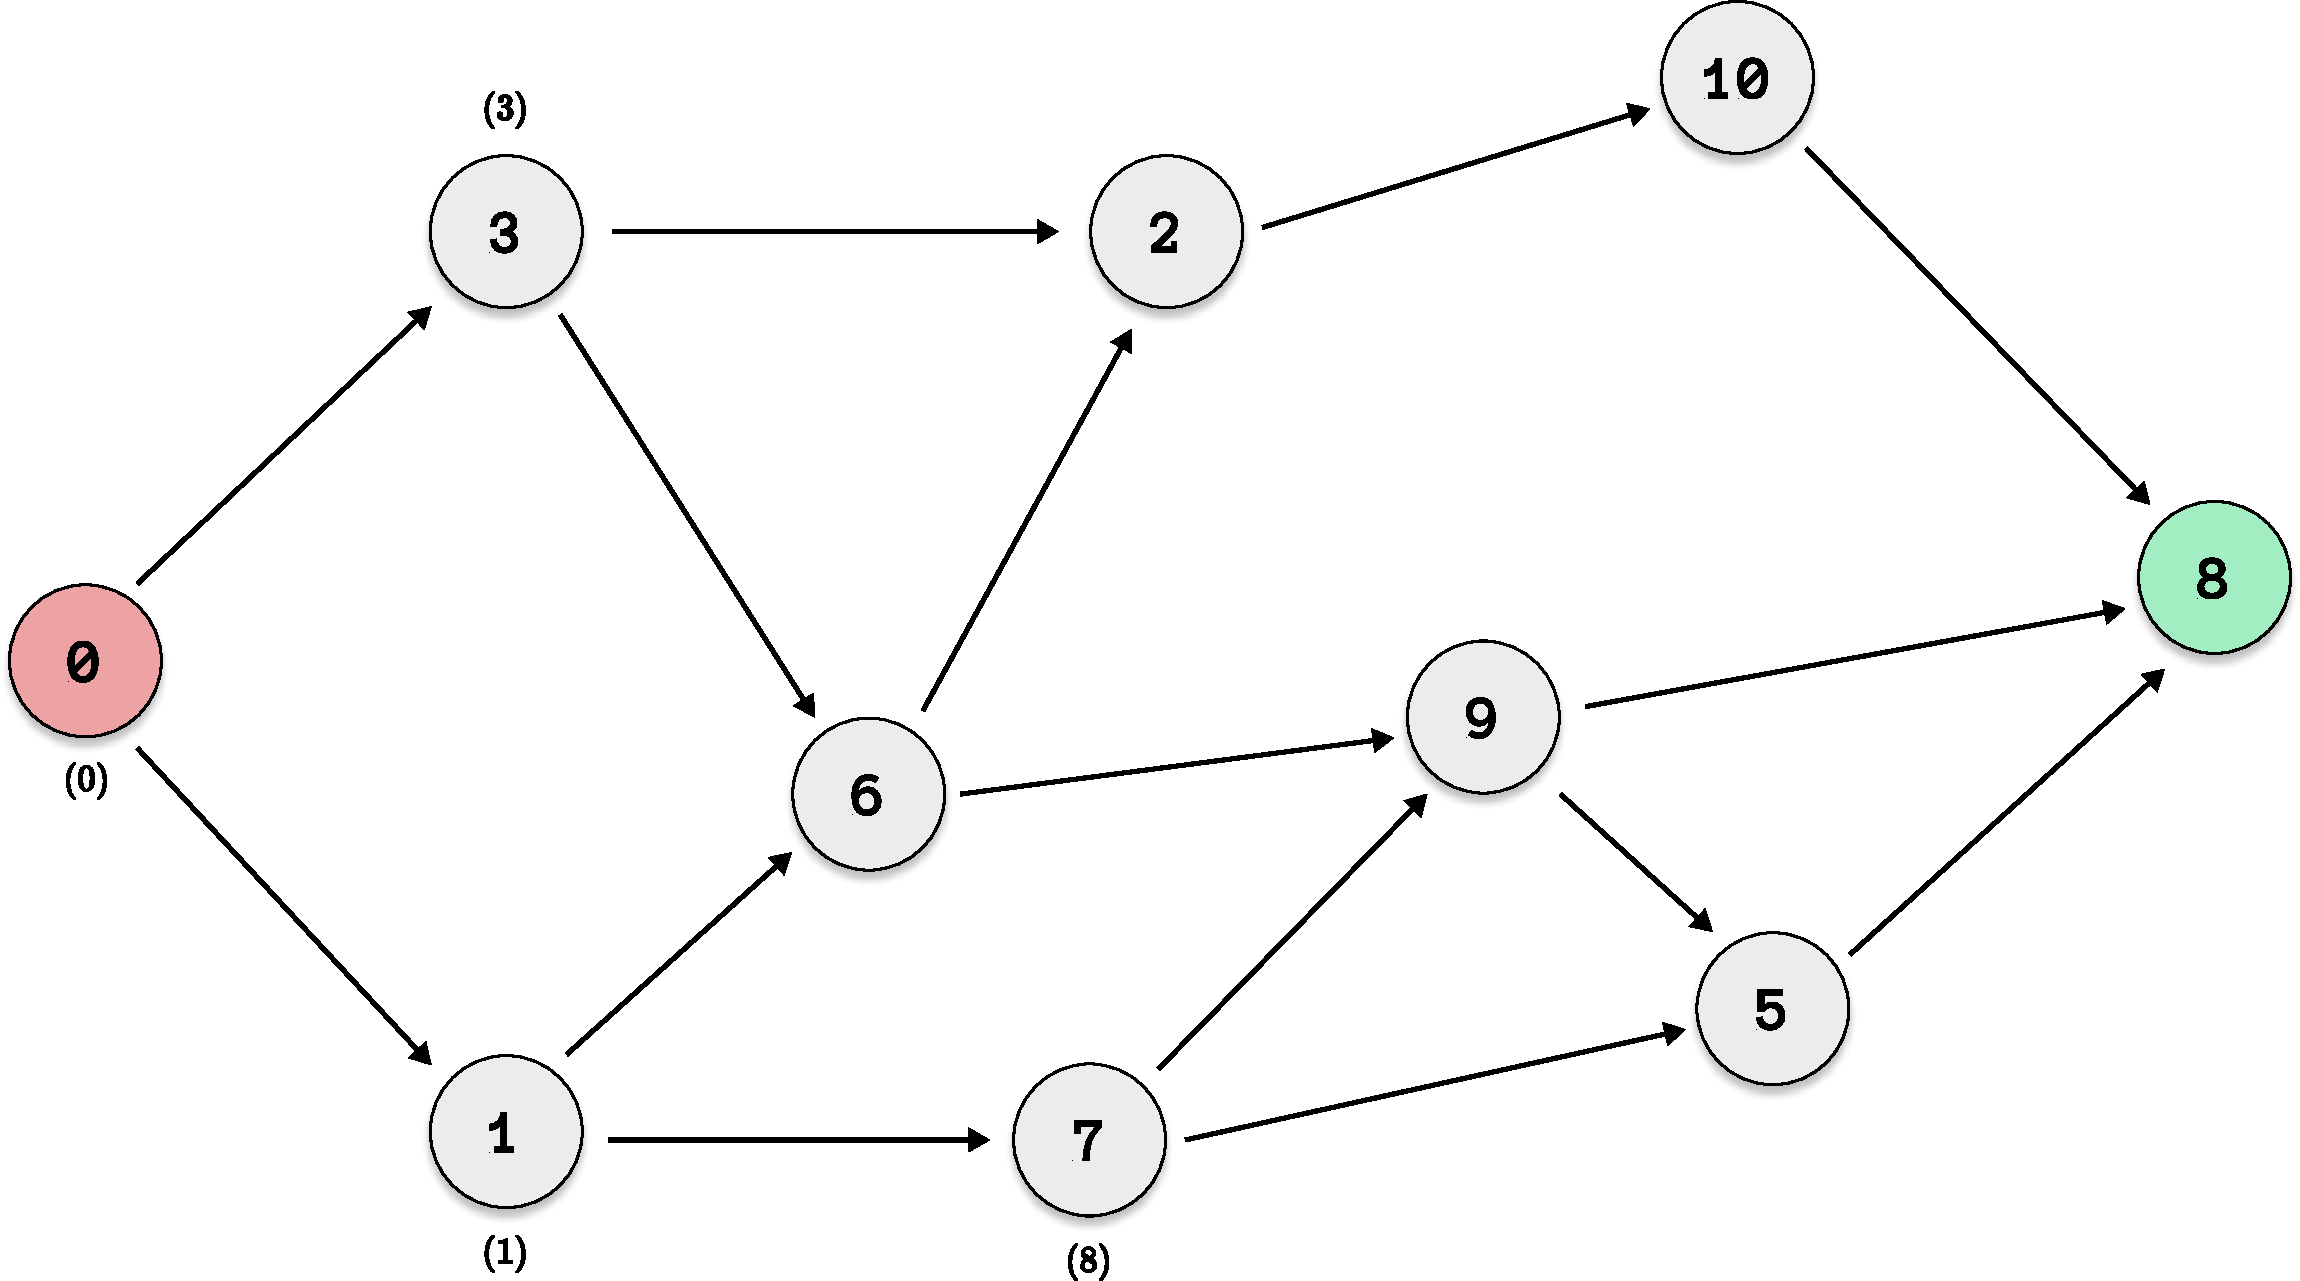
\includegraphics[width=0.9\textwidth]{assets/dag_explicit4.pdf}}
        \only<5>{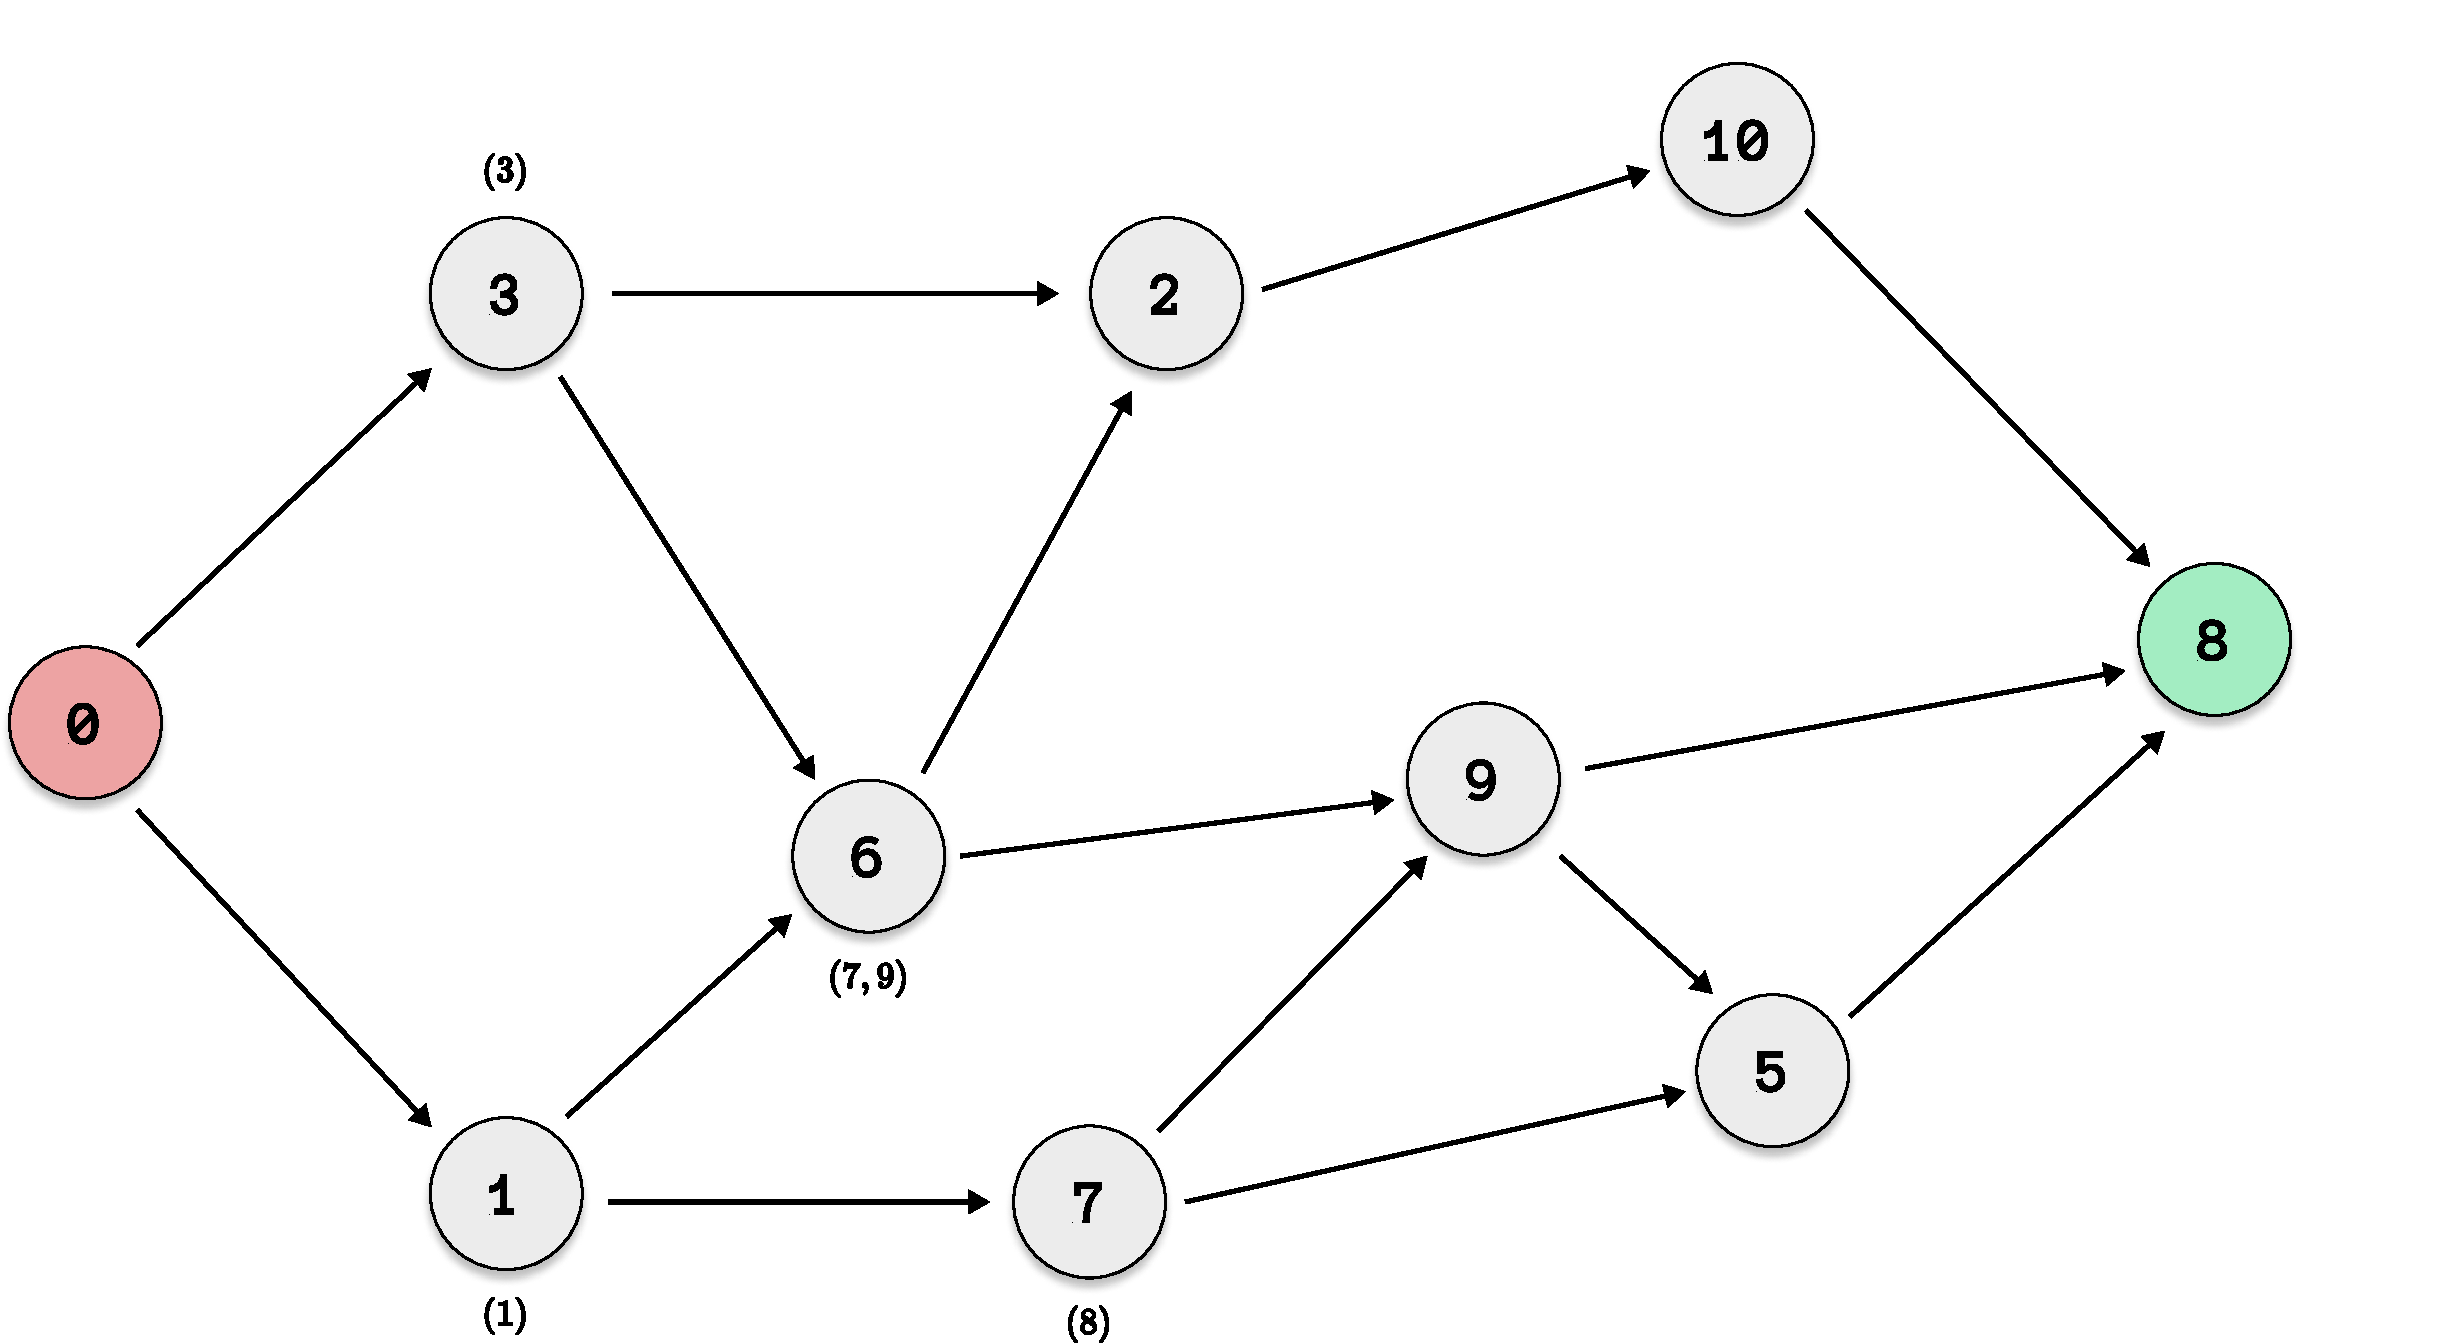
\includegraphics[width=0.9\textwidth]{assets/dag_explicit5.pdf}}
        \only<6>{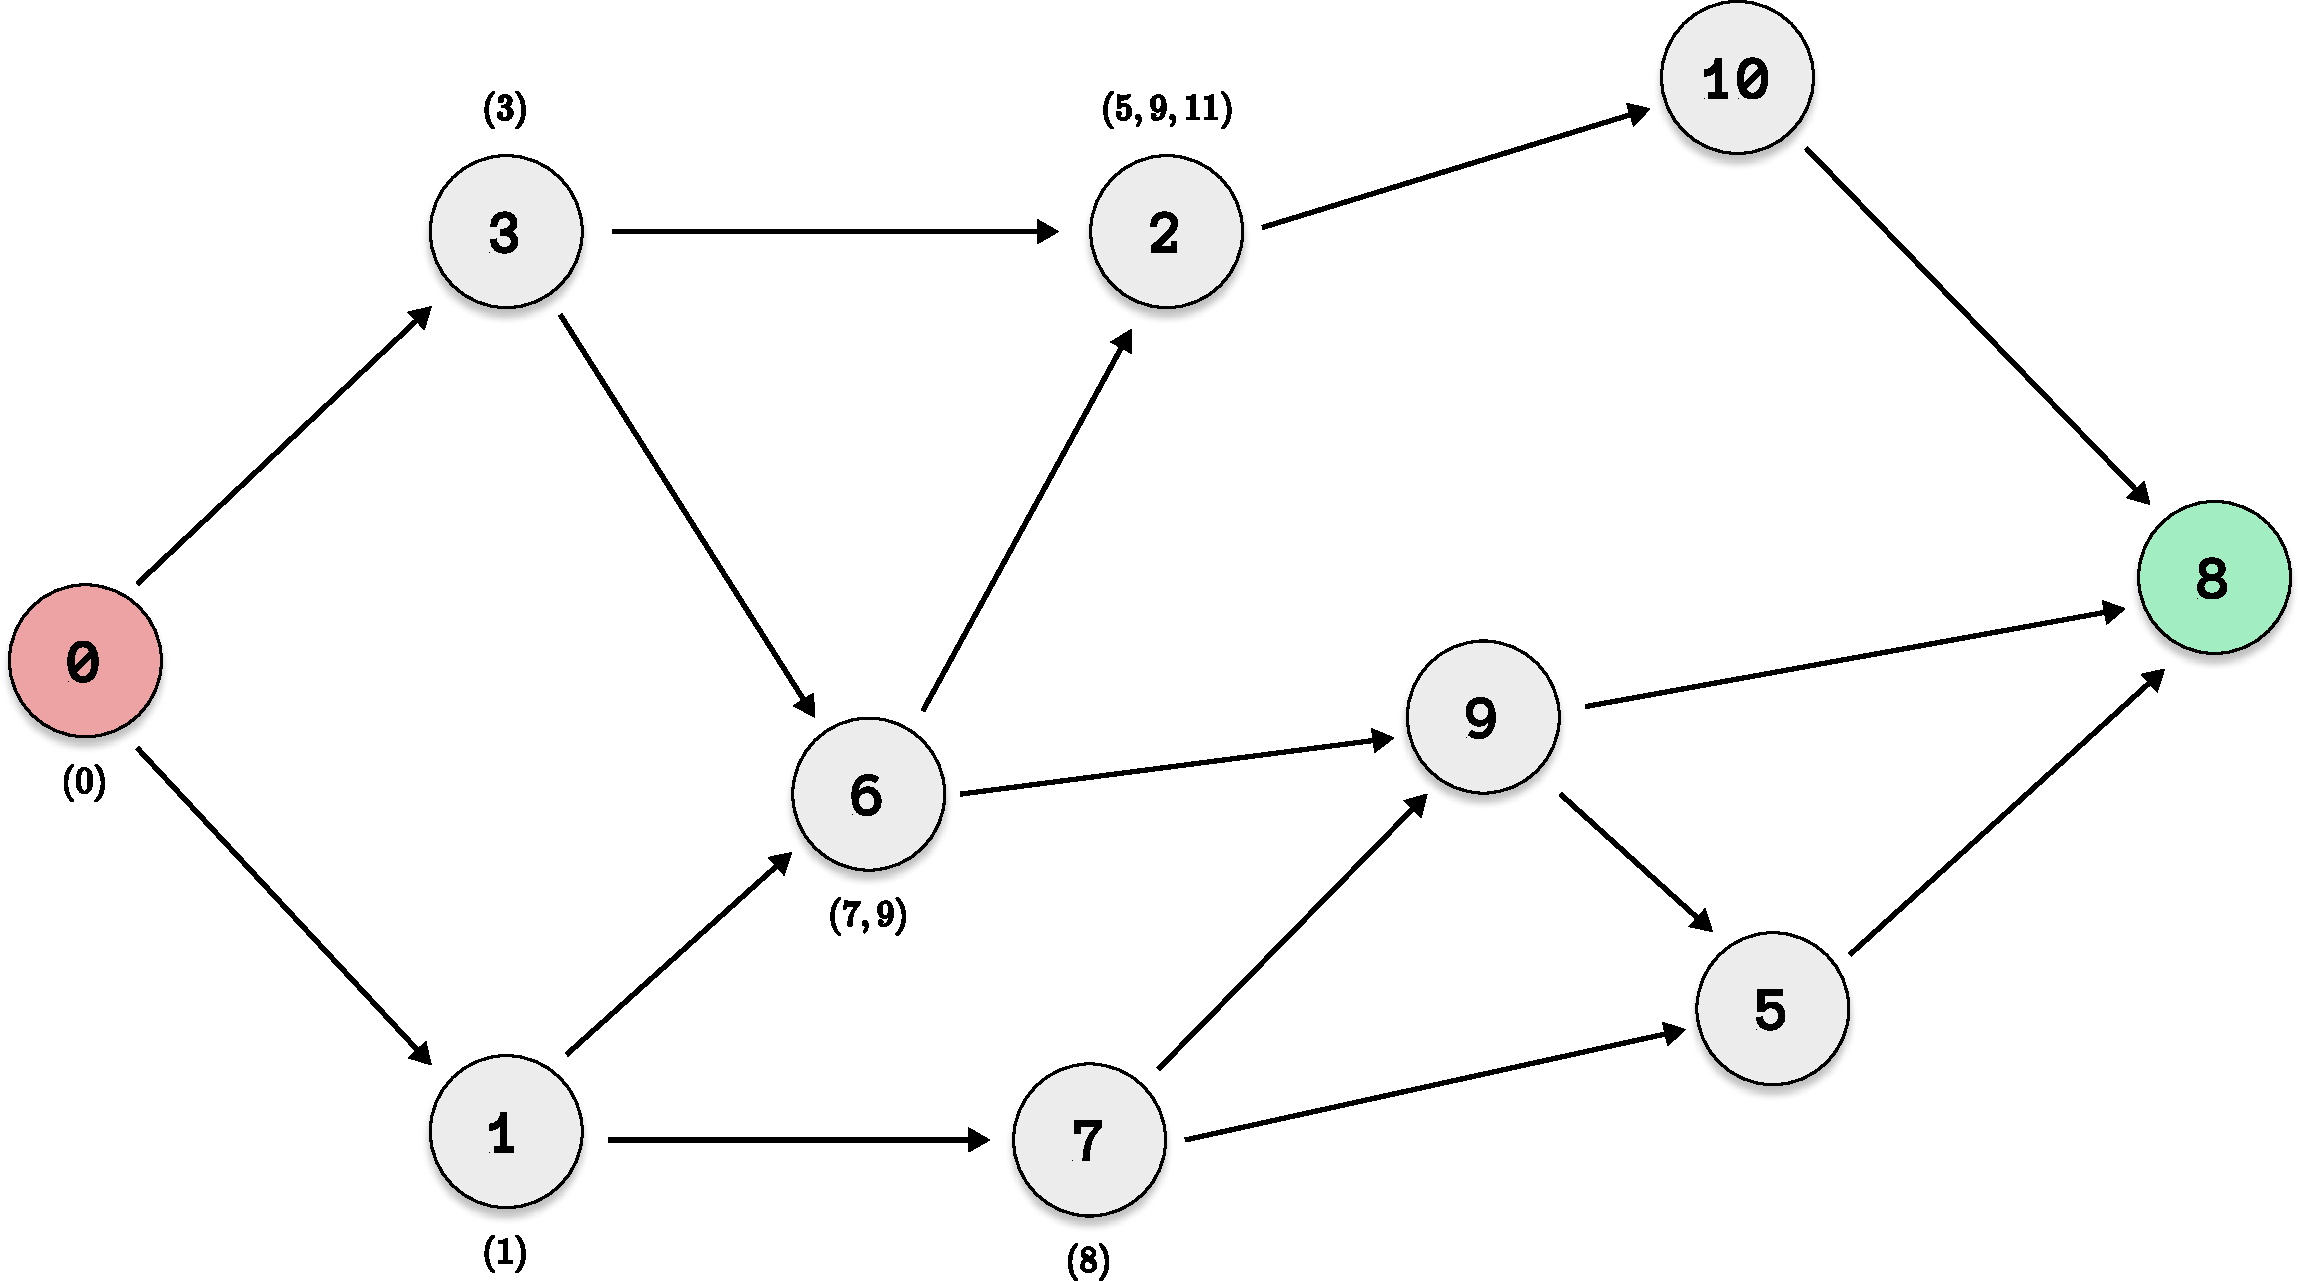
\includegraphics[width=0.9\textwidth]{assets/dag_explicit6.pdf}}
        \only<7>{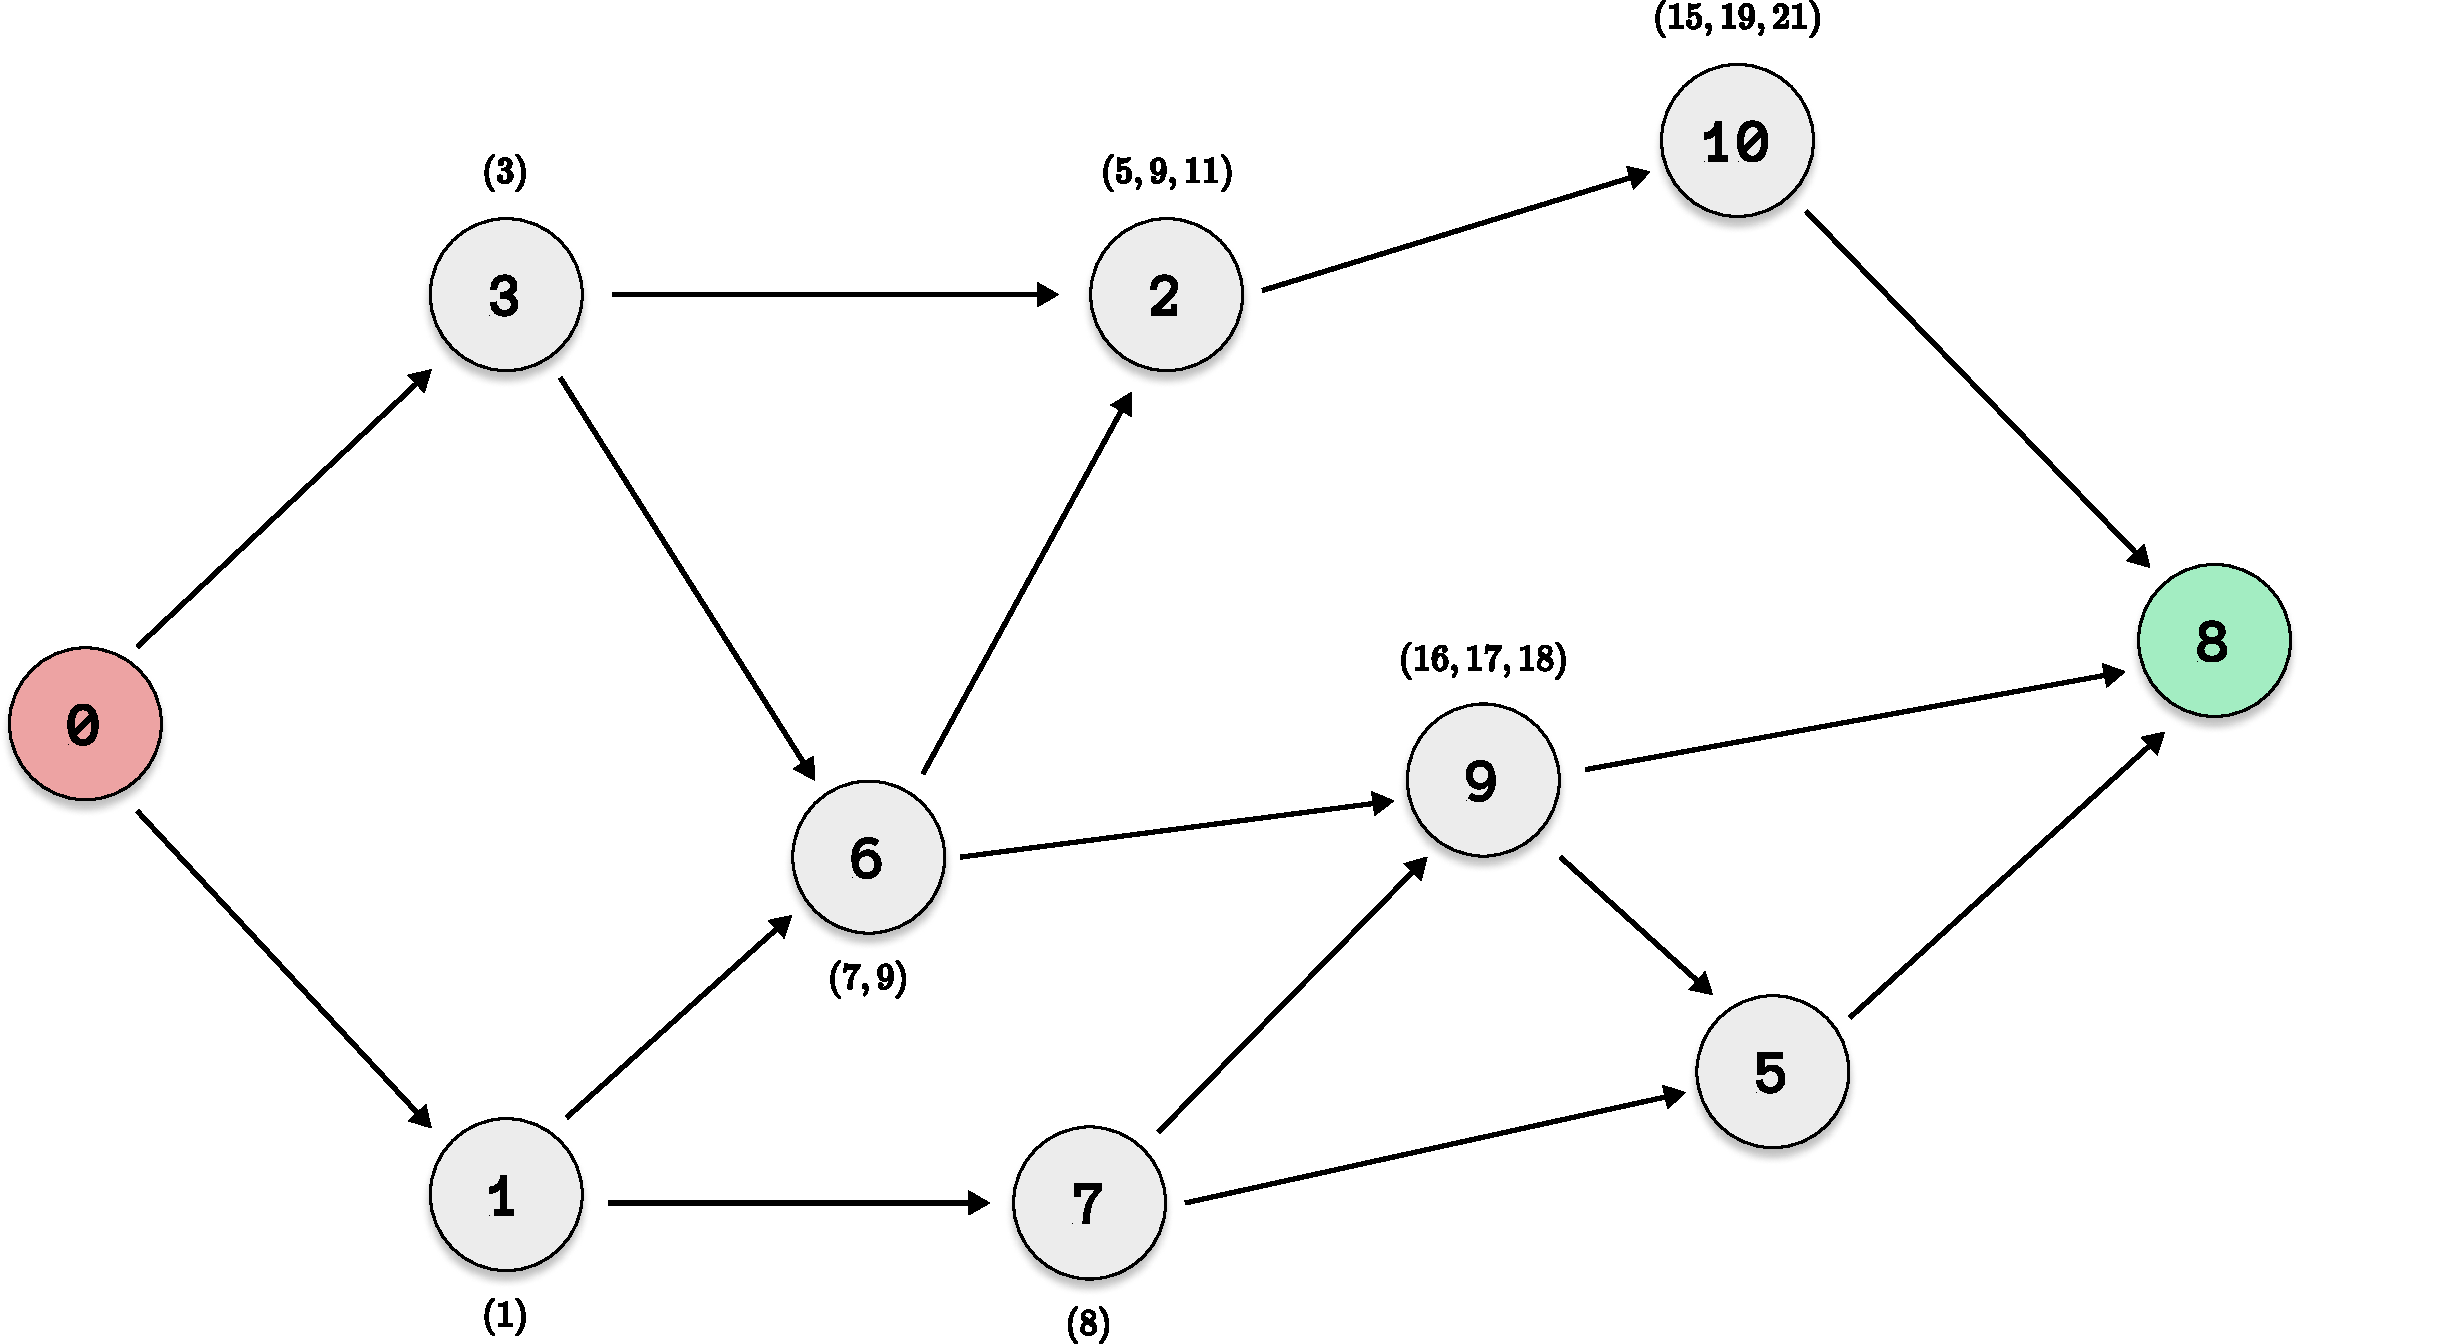
\includegraphics[width=0.9\textwidth]{assets/dag_explicit7.pdf}}
        \only<8>{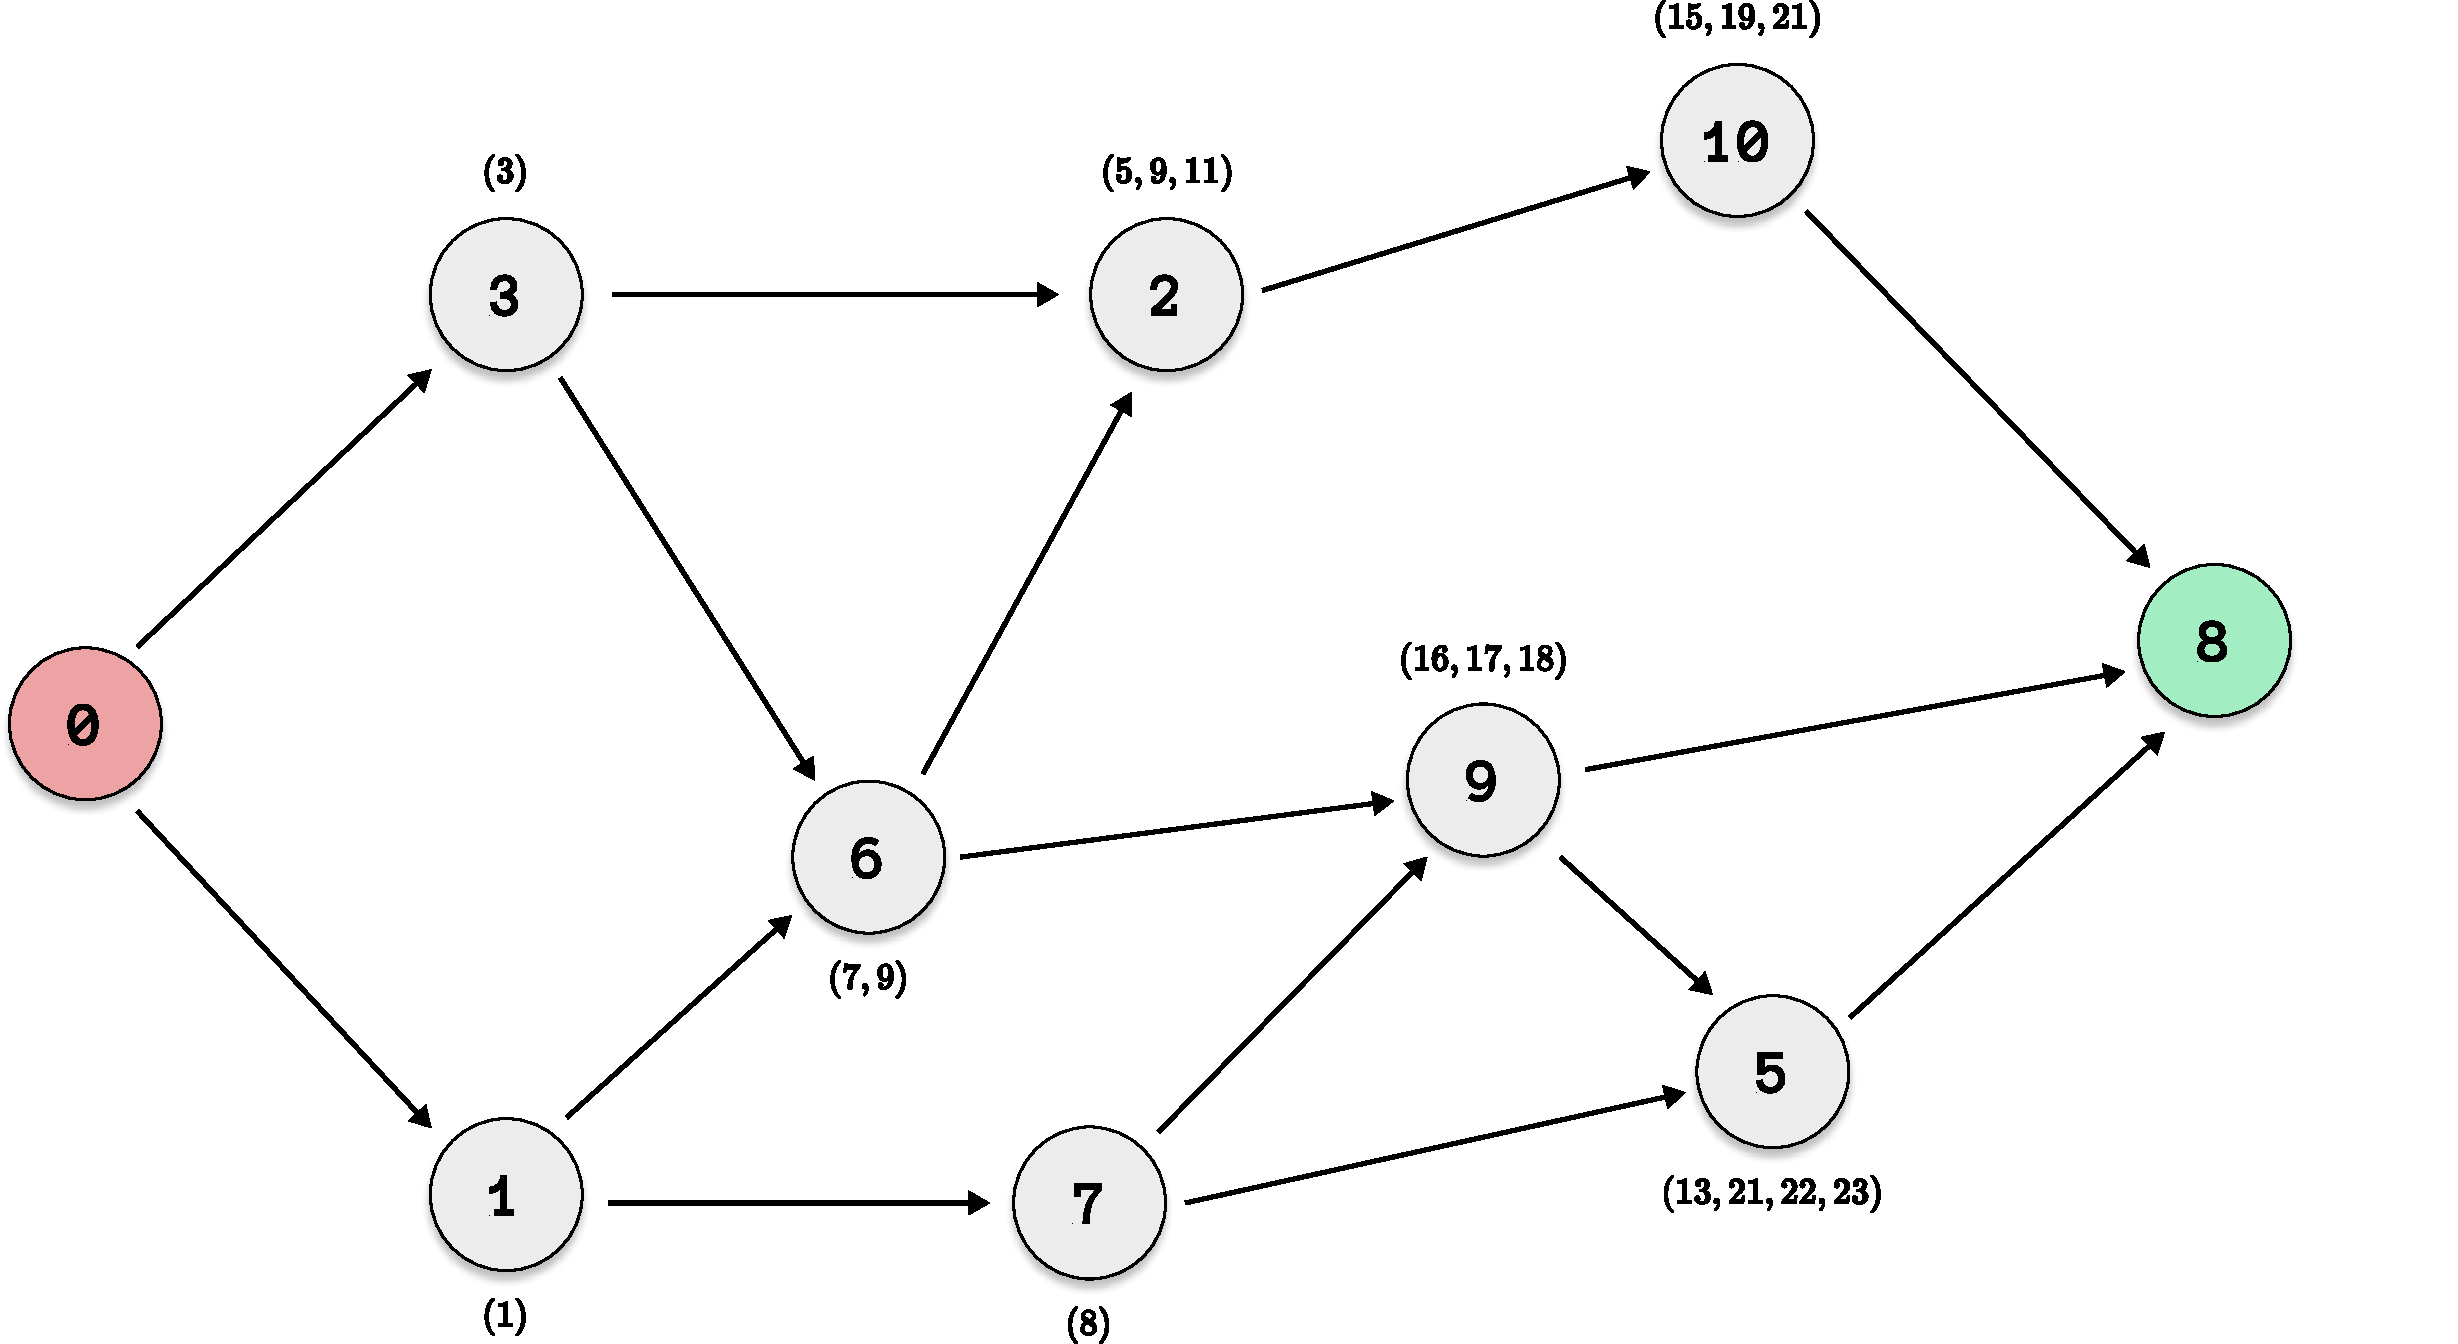
\includegraphics[width=0.9\textwidth]{assets/dag_explicit8.pdf}}
        \only<9>{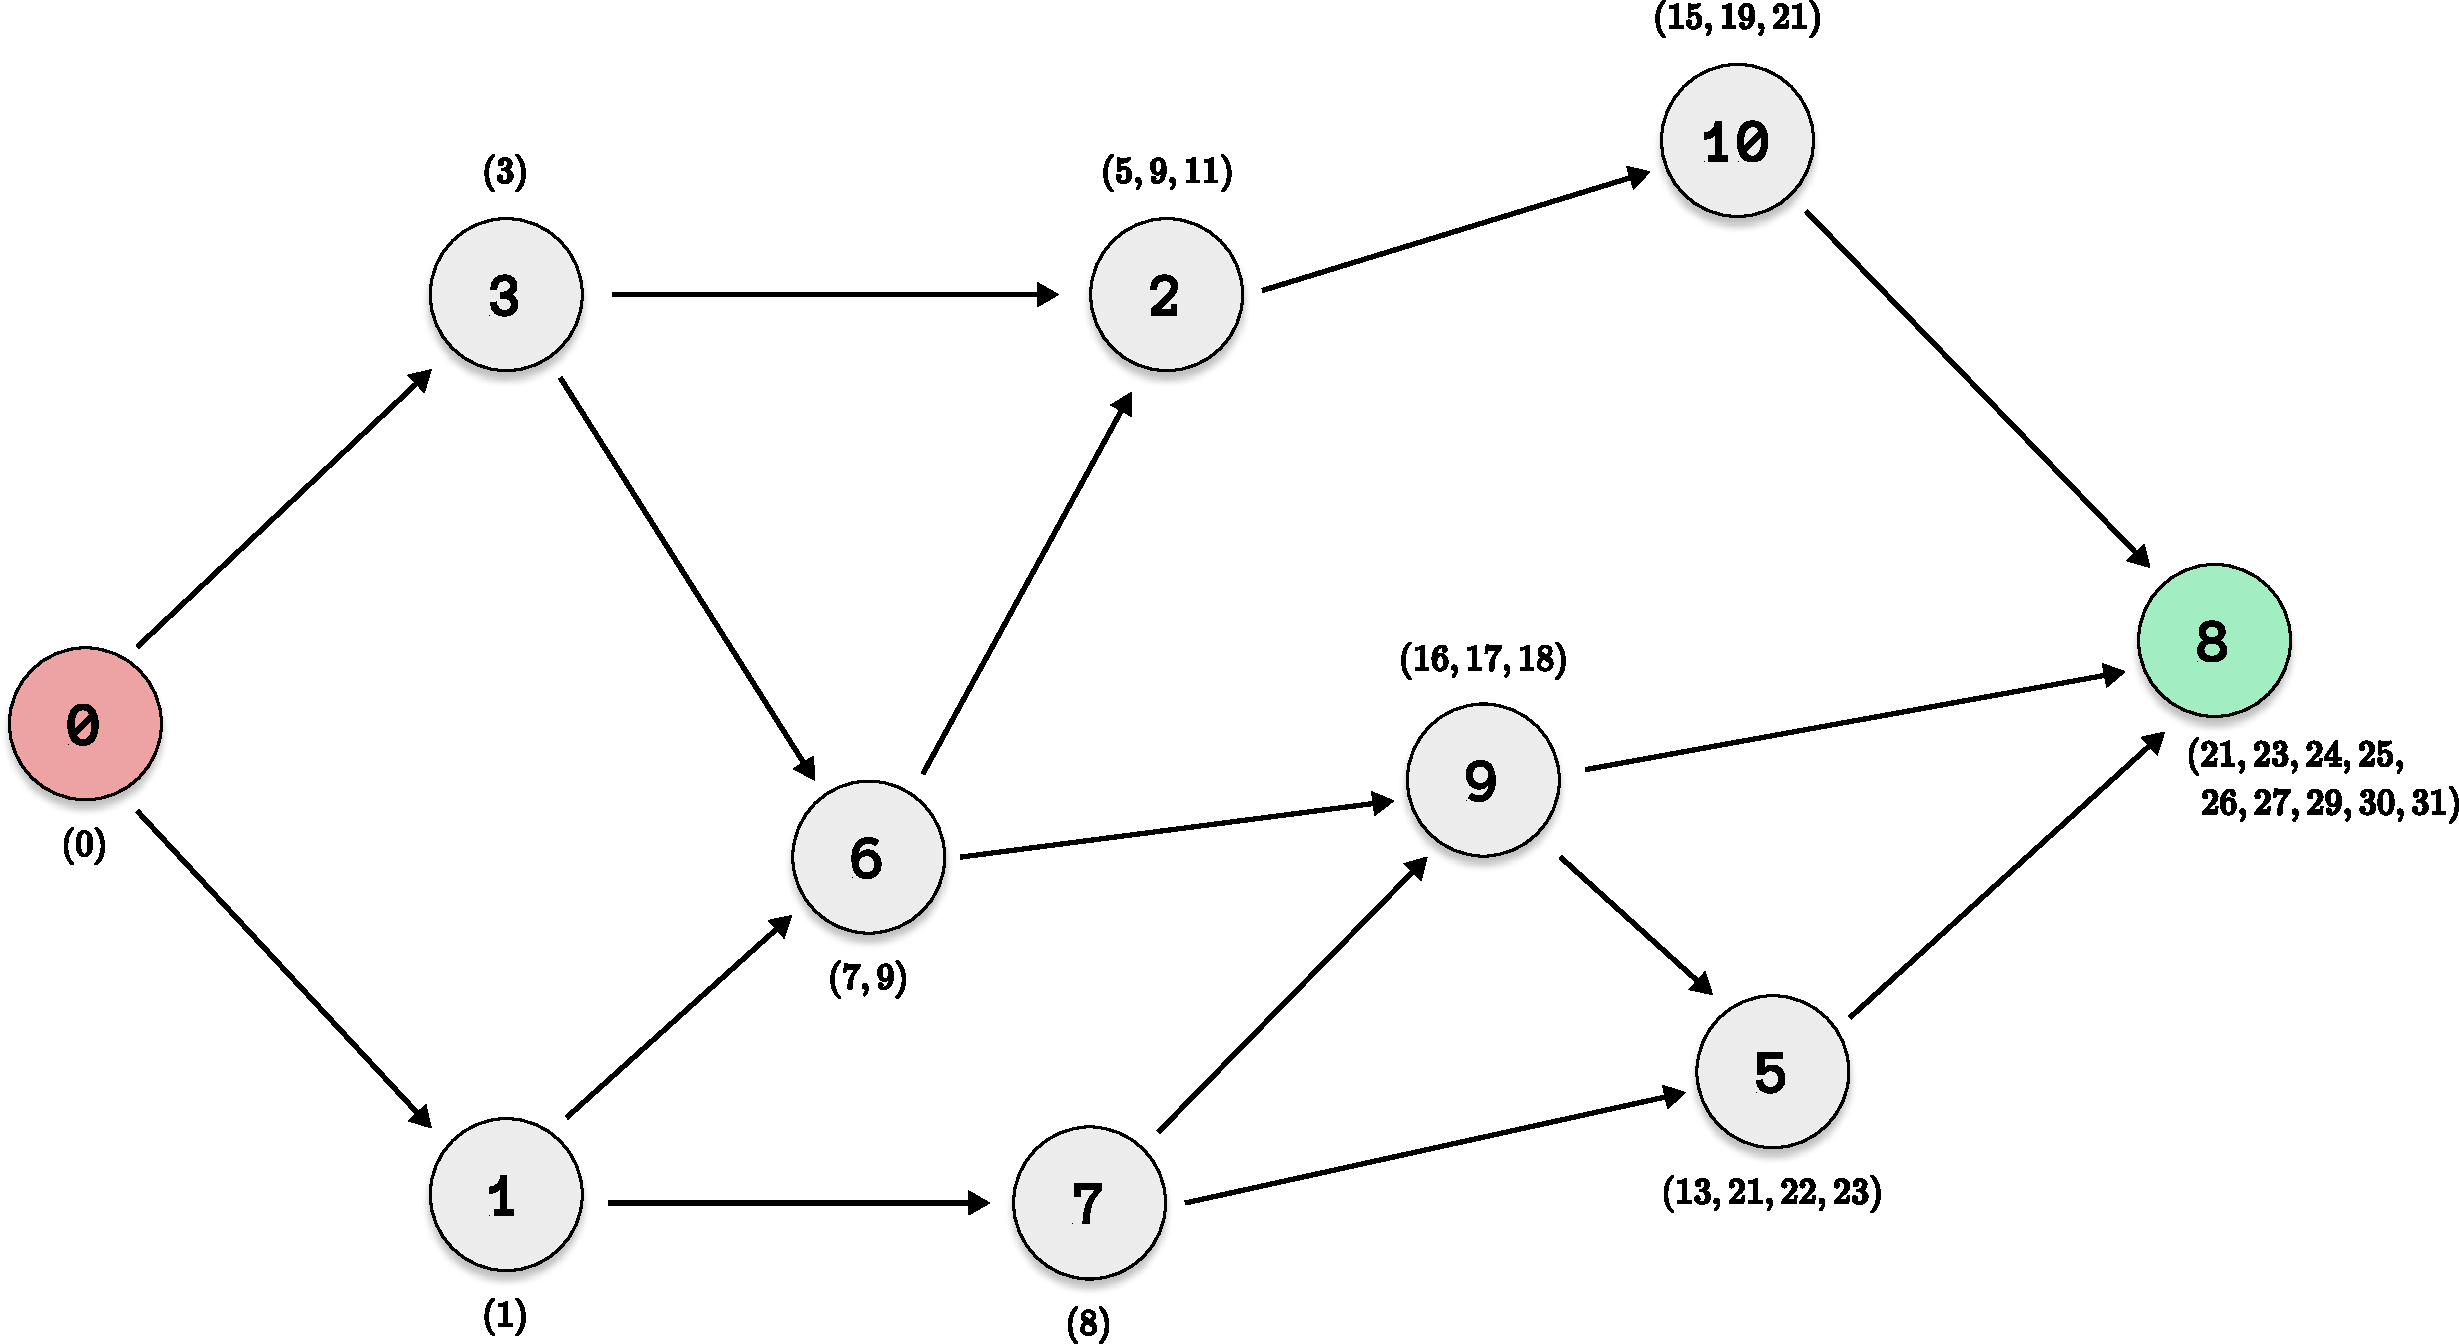
\includegraphics[width=0.9\textwidth]{assets/dag_explicit_final.pdf}}
    \end{figure}
    % \begin{figure}[h!]
    %     \centering
    %     % \resizebox{0.9\textwidth}{!}{% Reduced size slightly to make space for labels
    %     %     \begin{tikzpicture}[
    %     %         node distance=1.5cm and 1cm,
    %     %         base_node/.style={circle, draw=black, thick, minimum size=8mm, inner sep=0pt, font=\sffamily},
    %     %         root_node/.style={base_node, fill=red!60, text=black},
    %     %         % Definizione stile per label O-set
    %     %         data_label/.style={font=\tiny\ttfamily, text=blue!80!black, anchor=north},
    %     %         edge_style/.style={->, >={Stealth[length=2mm]}, thick, draw=black}
    %     %         ]

    %     %         % Nodes (pesi dentro)
    %     %         \node[root_node] (0) at (0, 2) {0};
    %     %         \node[base_node] (1) at (1.5, 0) {1};
    %     %         \node[base_node] (3) at (1.5, 4) {3};
    %     %         \node[base_node] (6) at (3.5, 1.5) {6};
    %     %         \node[base_node] (7) at (4.5, 0) {7};
    %     %         \node[base_node] (2) at (5.5, 4) {2};
    %     %         \node[base_node] (9) at (6.5, 2) {9};
    %     %         \node[base_node] (5) at (9, 0.5) {5};
    %     %         \node[base_node] (10) at (8.5, 5) {10};
    %     %         \node[base_node] (8) at (11, 3) {8};

    %     %         % Edges
    %     %         \draw [edge_style] (0) -- (1); \draw [edge_style] (0) -- (3);
    %     %         \draw [edge_style] (1) -- (6); \draw [edge_style] (1) -- (7);
    %     %         \draw [edge_style] (3) -- (2); \draw [edge_style] (3) -- (6);
    %     %         \draw [edge_style] (6) -- (2); \draw [edge_style] (6) -- (9);
    %     %         \draw [edge_style] (7) -- (5); \draw [edge_style] (7) -- (9);
    %     %         \draw [edge_style] (2) -- (10);
    %     %         \draw [edge_style] (9) -- (5); \draw [edge_style] (9) -- (8);
    %     %         \draw [edge_style] (10) -- (8); \draw [edge_style] (5) -- (8);

    %     %         % O-Set Labels appearing step-by-step
    %     %         \node<1->[data_label, red] at (0.south) {\{0\}};
    %     %         \node<2->[data_label] at (1.south) {\{1\}};
    %     %         \node<2->[data_label] at (3.south) {\{3\}};
    %     %         \node<3->[data_label] at (7.south) {\{8\}};
    %     %         \node<4->[data_label] at (6.south) {\{7, 9\}};
    %     %         \node<5->[data_label] at ([xshift=0.3cm]2.south) {\{5, 9, 11\}};
    %     %         \node<6->[data_label] at ([yshift=-0.1cm, xshift=0.2cm]9.south) {\{16, 17, 18\}};
    %     %         \node<7->[data_label] at (10.south) {\{15, 19, 21\}};
    %     %         \node<8->[data_label] at (5.south) {\{13, 21, 22, 23\}};
    %     %         \node<9->[data_label, align=center] at ([yshift=-0.2cm, xshift=0.4cm]8.south) {\{21, 23, 24, 25, \\ 26, 27, 29, 30, 31\}};

    %     %     \end{tikzpicture}
    %     % } % End resizebox
    % \end{figure}
\end{frame}

% --- SLIDE 15: The Rank Query - Concept ---
\begin{frame}{The Rank Query on Weighted DAGs}
    \framesubtitle{What Values are "Active" at Node N?}
    % \begin{block}{Motivation}
    %     The $\mathcal{O}$-Set ($\mathcal{O}_N$) tells us the \alert{final} path weights ending at node $N$.
    %     But we want to know which cumulative weight values are relevant \alert{during} the "processing" step associated with node $N$ itself.
    % \end{block}
    \begin{block}{Rank Query on a Node $N$: $\mathrm{rank}_G(N)$}
        \begin{enumerate}
            \item Returns a representation of a set of integers derived from the $\mathcal{O}$-set $\mathcal{O}_N$.
                  \[ S_N = \bigcup_{x \in \mathcal{O}_N} \{ z \in \mathbb{N}_0 \mid \max(0, x - w(N) + 1) \le z \le x \}. \]
                  \vspace{-1em}
                  \pause
            \item These intervals are then maximally merged. The query $\mathrm{rank}_G(N)$ returns a \alert{minimal collection of disjoint closed integer intervals}
                  \[ \mathcal{R}_N = \{[l_1, r_1], [l_2, r_2], \dots, [l_p, r_p]\} \]
                  such that their union exactly covers $S_N$.
                  % \item Return the result as a \alert{minimal set of disjoint intervals} $\mathcal{R}_N$.
        \end{enumerate}
    \end{block}
    $\mathcal{R}_N$ captures the range of possible cumulative sums during the \emph{activity} at node $N$

\end{frame}


% \subsection{Succinct Structure and Queries}
% --- SLIDE 16: The Challenge and The Core Idea ---
% \begin{frame}{The Challenge: Storing Path Information}
%     \framesubtitle{$\mathcal{O}$-Sets Can Be Huge!}

%     \begin{itemize}
%         \item \textbf{Problem}: The size $|\mathcal{O}_v|$ can grow very large!
%         \item \textbf{Question:} Can we represent the necessary information more compactly?
%     \end{itemize}

%     \begin{alertblock}<2->{Core Idea: Partitioning + Indirection}
%         \begin{enumerate}
%             \item<2-> Partition vertices $V$ into:
%                 \begin{itemize}
%                     \item \textbf{Explicit Vertices ($V_E$):} Typically sinks. Store their $\mathcal{O}_v$ directly.
%                     \item \textbf{Implicit Vertices ($V_I$):} All others. Do \emph{not} store $\mathcal{O}_v$ directly.
%                 \end{itemize}
%             \item<3-> For implicit $v \in V_I$, reconstruct $\mathcal{O}_v$ on-the-fly using:
%                 \begin{itemize}
%                     \item A chosen \textbf{designated successor} $\sigma(v) \in Succ(v)$.
%                     \item An \textbf{offset sequence} $\mathcal{J}_v$ stored at $v$.
%                 \end{itemize}
%         \end{enumerate}
%     \end{alertblock}

% \end{frame}


\begin{frame}{The Challenge: Storing Path Information}
    \framesubtitle{$\mathcal{O}$-Sets Can Be Huge!}

    % Problema e Domanda rimangono uguali
    \begin{itemize}
        \item \textbf{Problem}: The size $|\mathcal{O}_v|$ can grow very large!
        \item \textbf{Question:} Can we represent the necessary information more compactly?
    \end{itemize}


    \begin{alertblock}<2->{Core Idea: Partitioning + Indirection}
        Partition vertices $V$ into two types:
    \end{alertblock}
    \vspace{-1em}
    \begin{columns}[T] % T allinea al top
        \begin{column}{0.48\textwidth}
            \begin{block}<2->{1. Explicit Vertices ($V_E$)}
                \centering
                Store $\mathcal{O}_v$ directly. \\
                (\textit{Simple, but potentially large})
            \end{block}
            % \uncover<3->{\textbf{}
        \end{column}

        \begin{column}{0.48\textwidth}
            \begin{block}<2->{2. Implicit Vertices ($V_I$)}
                \centering
                Do \emph{not} store $\mathcal{O}_v$ explicitly \\
                (\textit{Reconstruct on-the-fly.})
            \end{block}
            \vspace{0.5em}
        \end{column}
    \end{columns}
    \uncover<3->{\textbf{Reconstruction for $v \in V_I$ using}:
        \begin{itemize}
            \item Designated Successor $\sigma(v)$
            \item Offset Sequence $\mathcal{J}_v$ (at $v$)
        \end{itemize}
    }
\end{frame}



% --- SLIDE 17: Successor Choice and Offset Sequence ---
\begin{frame}{Implicit Reconstruction: Successor \& Offset}
    \framesubtitle{How $V_I$ Nodes Refer to Others}

    \begin{block}{1. Designated Successor $\sigma(v)$ (for $v \in V_I$)}
        Which successor should $v$ point to?
        \textbf{Heuristic}: Choose $u = \sigma(v)$ that minimizes $|\mathcal{O}_u|$.
        \[ \sigma(v) \in \underset{u \in Succ(v)}{\operatorname{argmin}} \{ |\mathcal{O}_u| \}. \]
    \end{block}
    \begin{block}{2. Offset Sequence $\mathcal{J}_v$ (for $v \in V_I$)}
        How to get $\mathcal{O}_v$ from $\mathcal{O}_{\sigma(v)}$? Let $u=\sigma(v)$.
        \begin{itemize}
            % \item Property: We know $|\mathcal{O}_v| \le |\mathcal{O}_u|$.
            \item \textbf{Relationship}: Each element $x_k \in \mathcal{O}_v$ comes from some $y_{j_k} \in \mathcal{O}_u$ via $x_k = y_{j_k} - w(u)$.
            \item \textbf{Offset Sequence $\mathcal{J}_v$}: Stores the index $j_k$ corresponding to each $x_k$.
                  \[ \mathcal{J}_v = (j_0, j_1, \dots, j_{m-1}), \quad \text{where } m = |\mathcal{O}_v| \]
        \end{itemize}
    \end{block}

\end{frame}

% % --- SLIDE 16: Structure Example Visualized (Corrected Labels & No Resize) ---
% \begin{frame}{Structure Example Visualized}
%     \framesubtitle{Applying the Partitioning and Pointers}
%     \begin{figure}[hbtp]
%         \centering
%         \only<1>{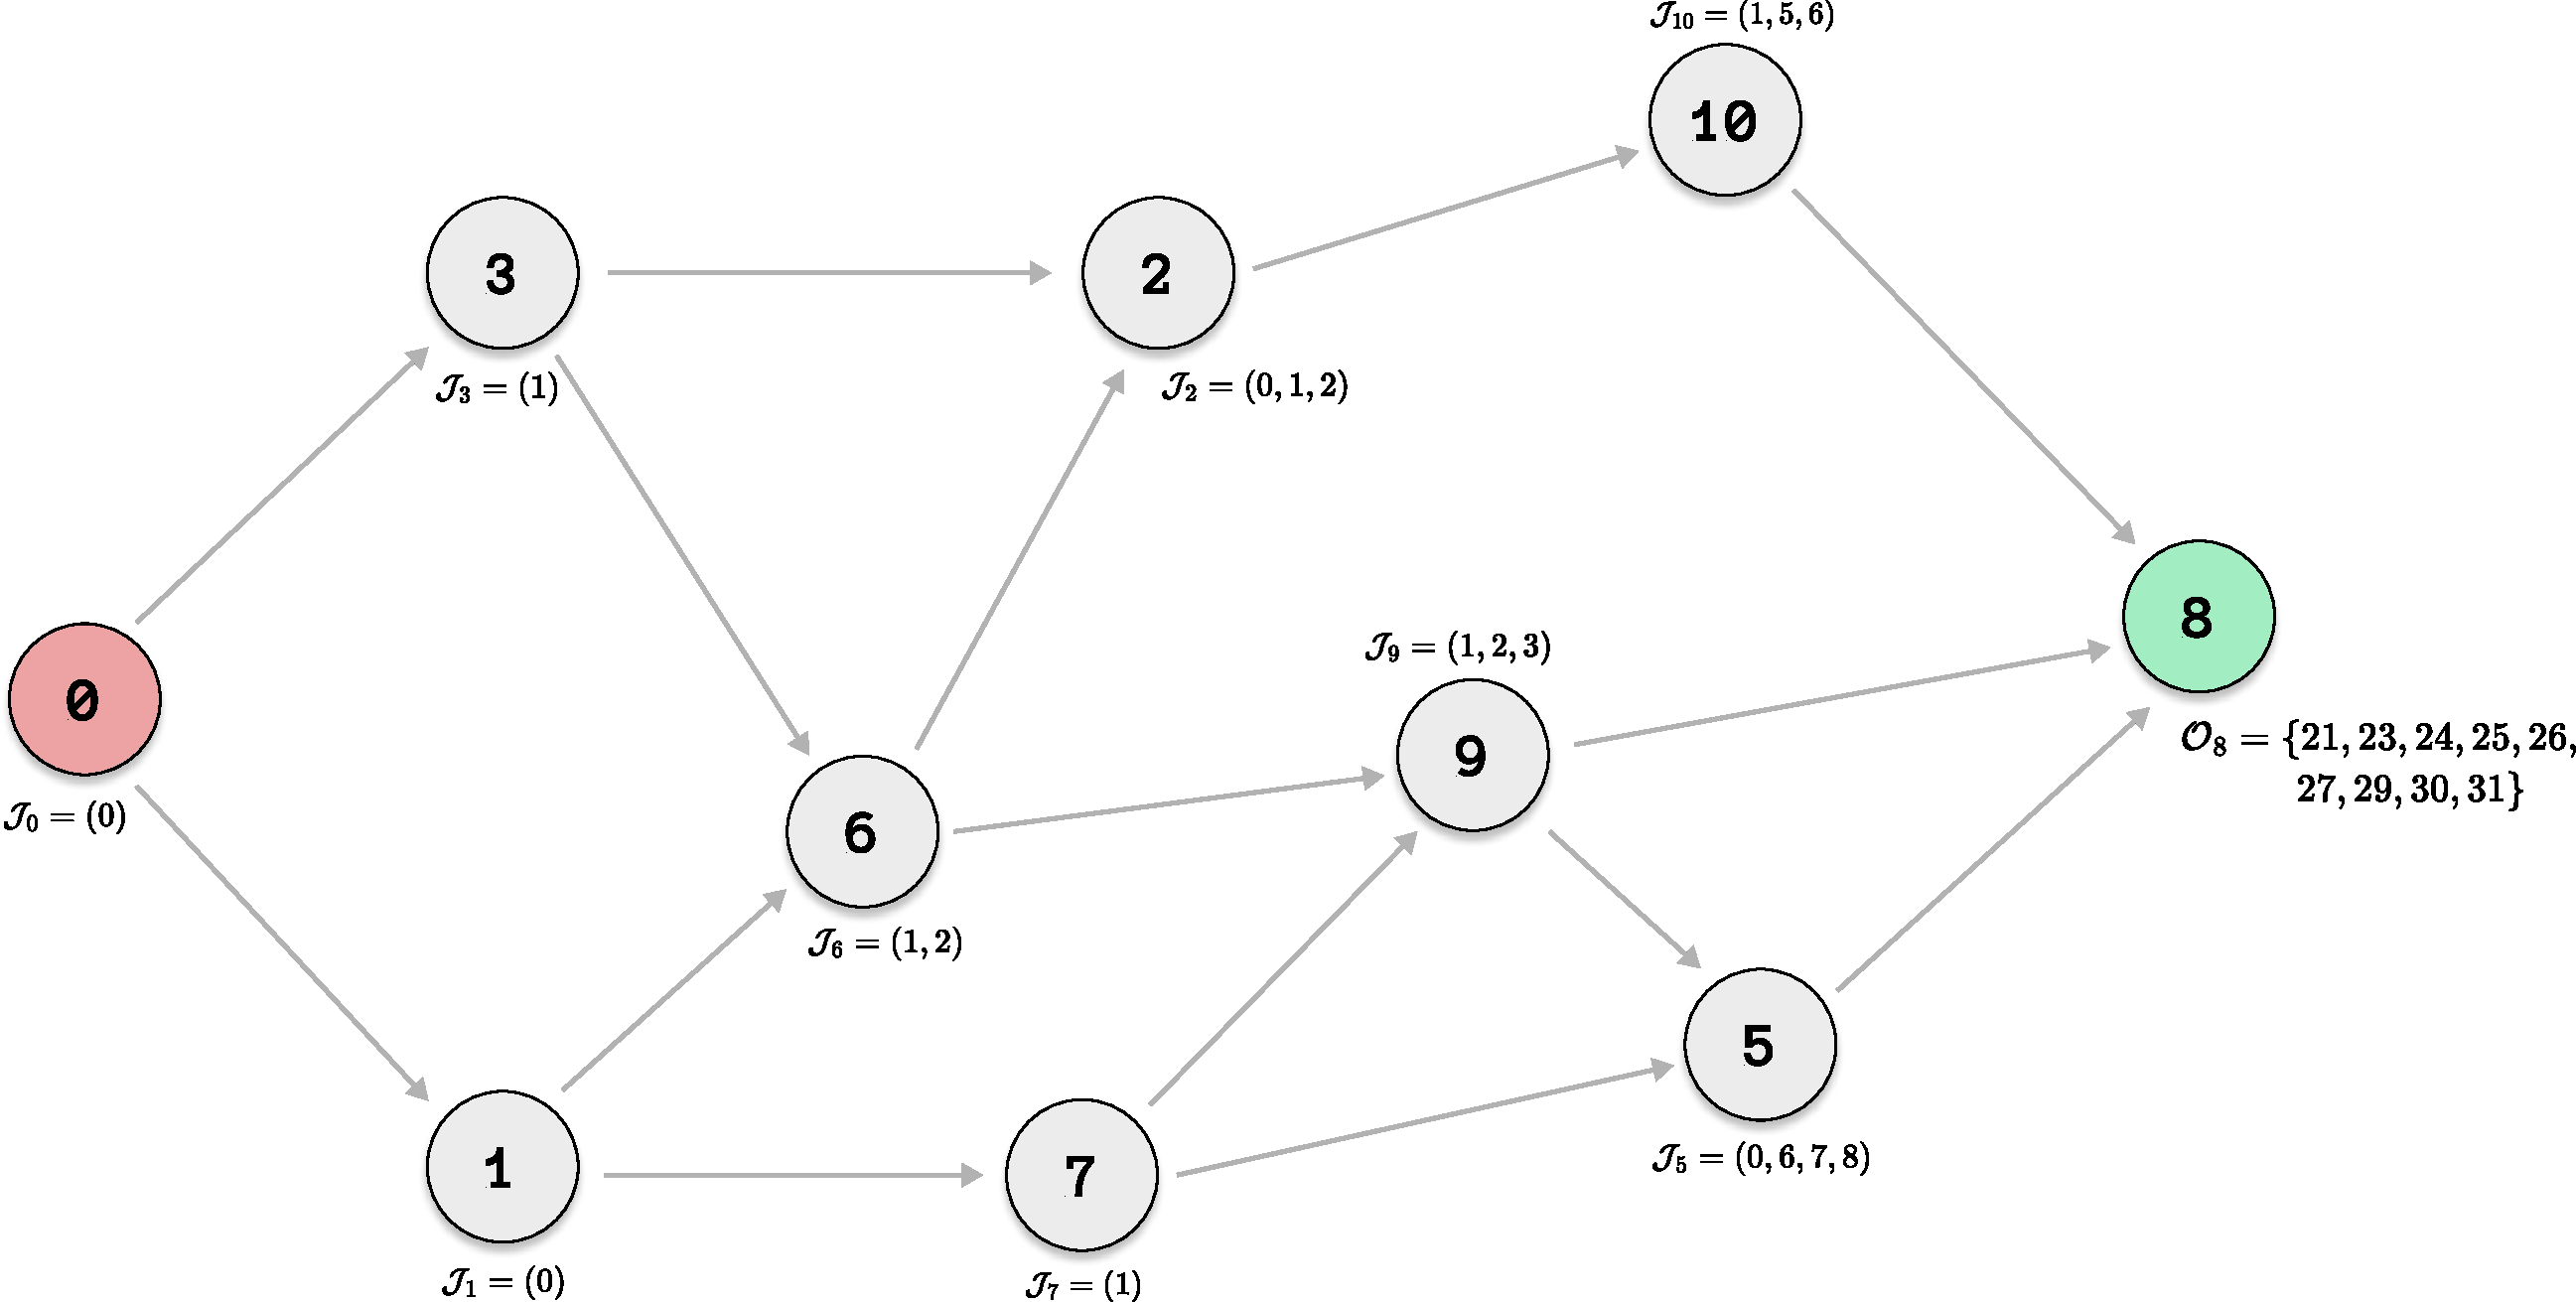
\includegraphics[width=0.9\textwidth]{../bachelor-thesis/TeX/assets/succinct-dag1.pdf}}
%         \only<2>{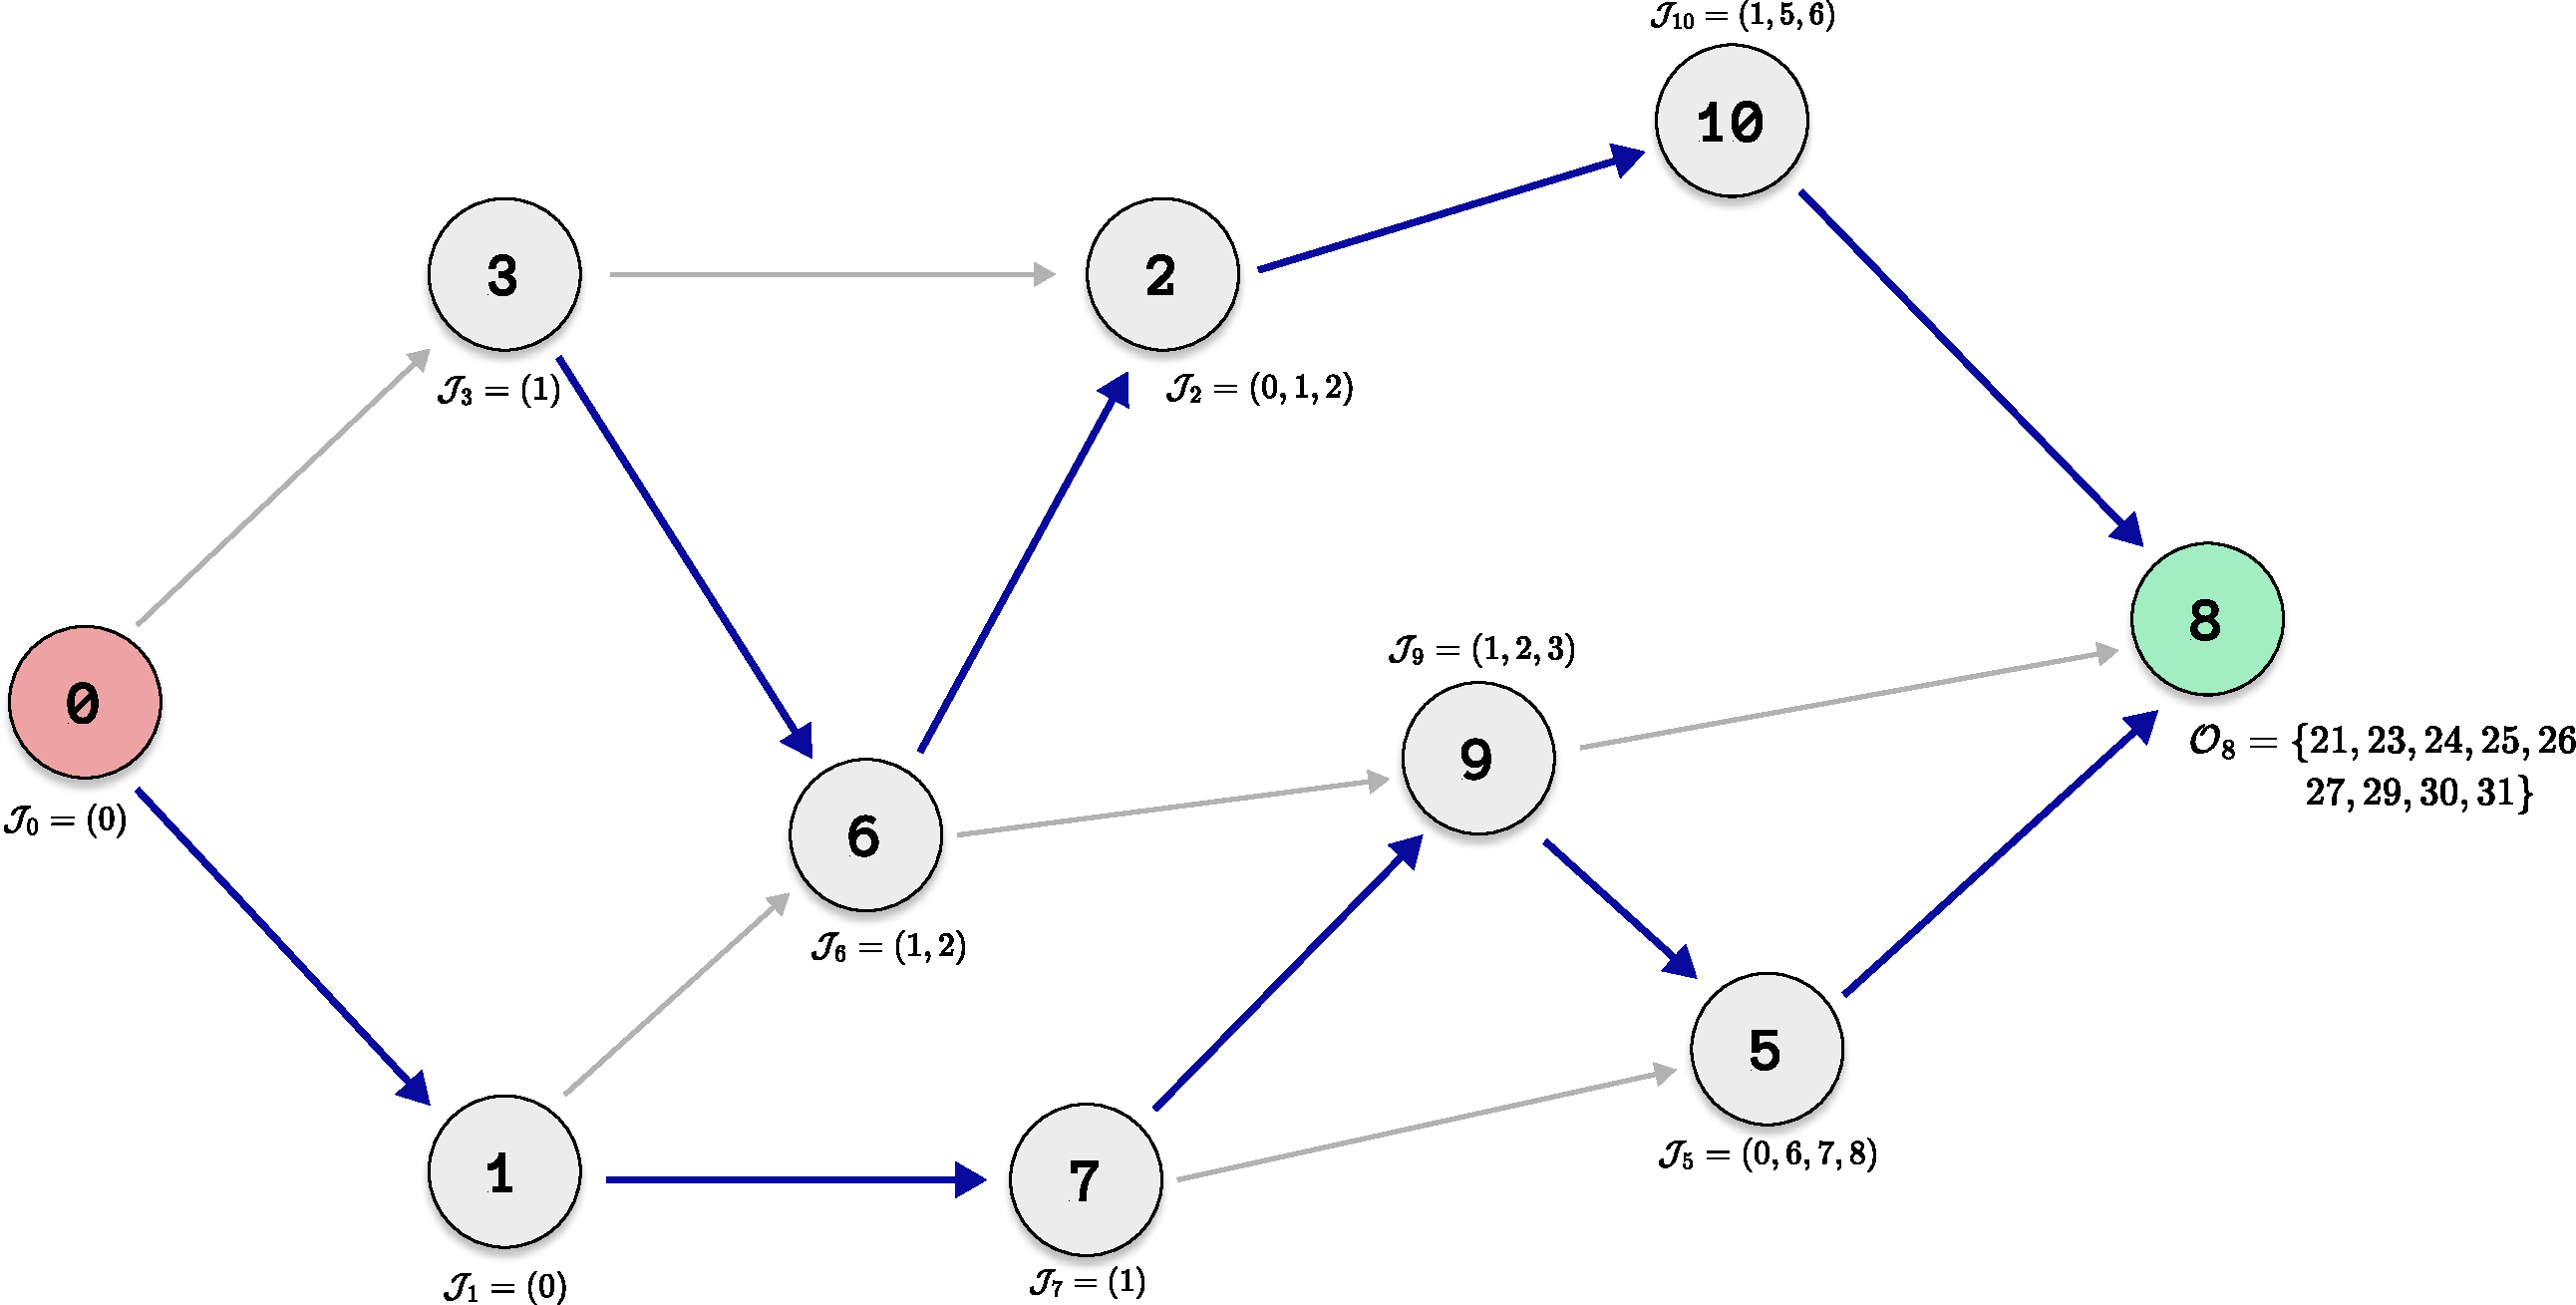
\includegraphics[width=0.9\textwidth]{../bachelor-thesis/TeX/assets/succinct-dag2.pdf}}
%     \end{figure}
% \end{frame}

% --- SLIDE 17: Example: Computing O_7[0] (Static Structure First) ---
\begin{frame}{Example: Computing $\mathcal{O}_7[0]$}
    \framesubtitle{Following the Successor Path: $7 \to 9 \to 5 \to 8$}
    \begin{figure}[hbtp]
        \centering
        % Replace TikZ with sequential images
        \only<1>{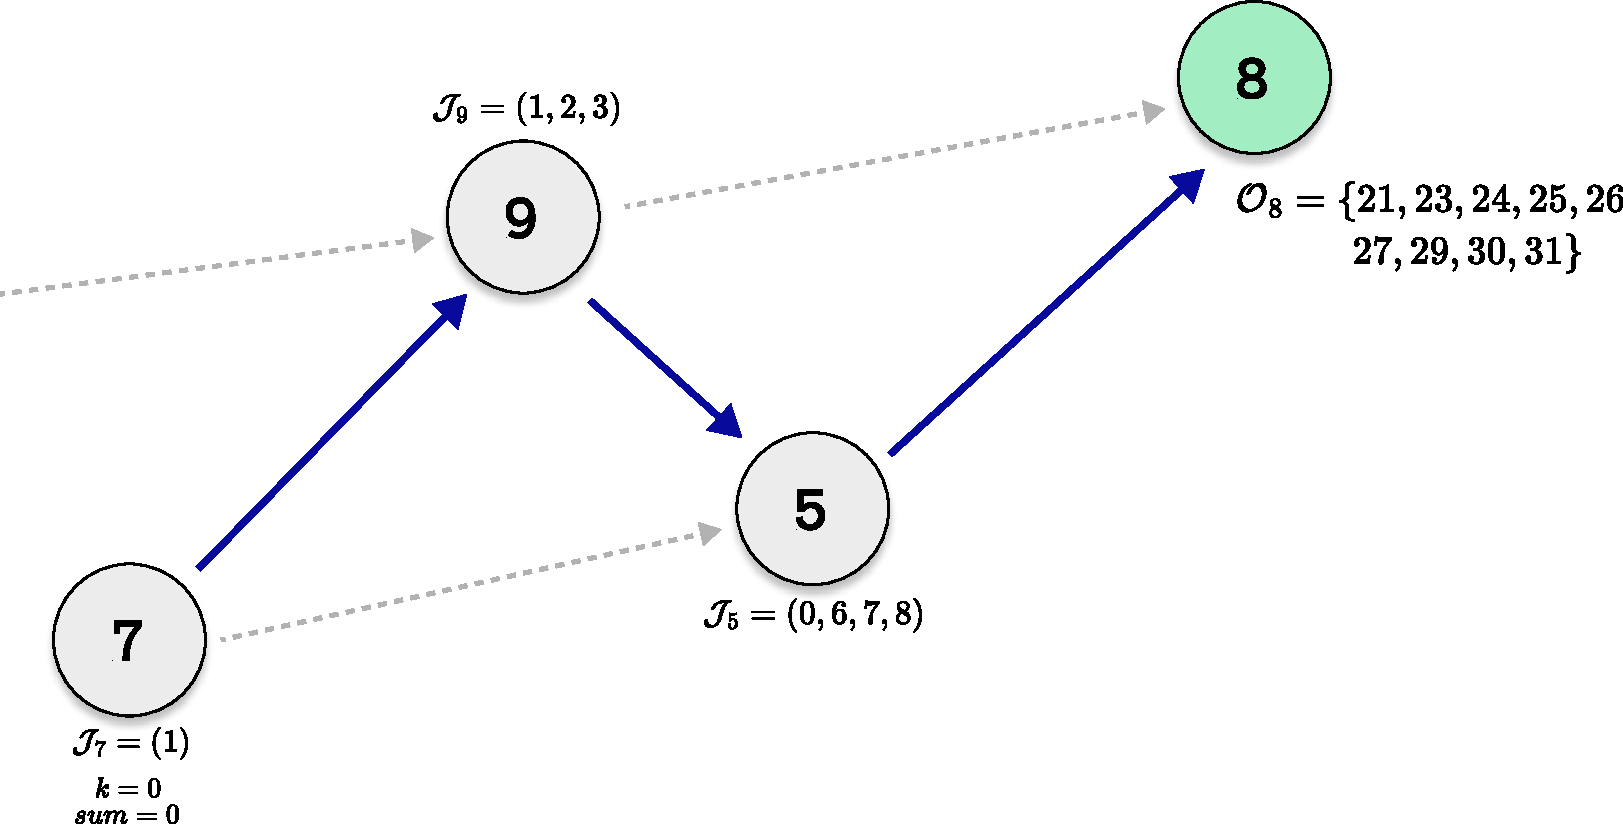
\includegraphics[width=0.9\textwidth]{assets/dag_query1.pdf}}
        \only<2>{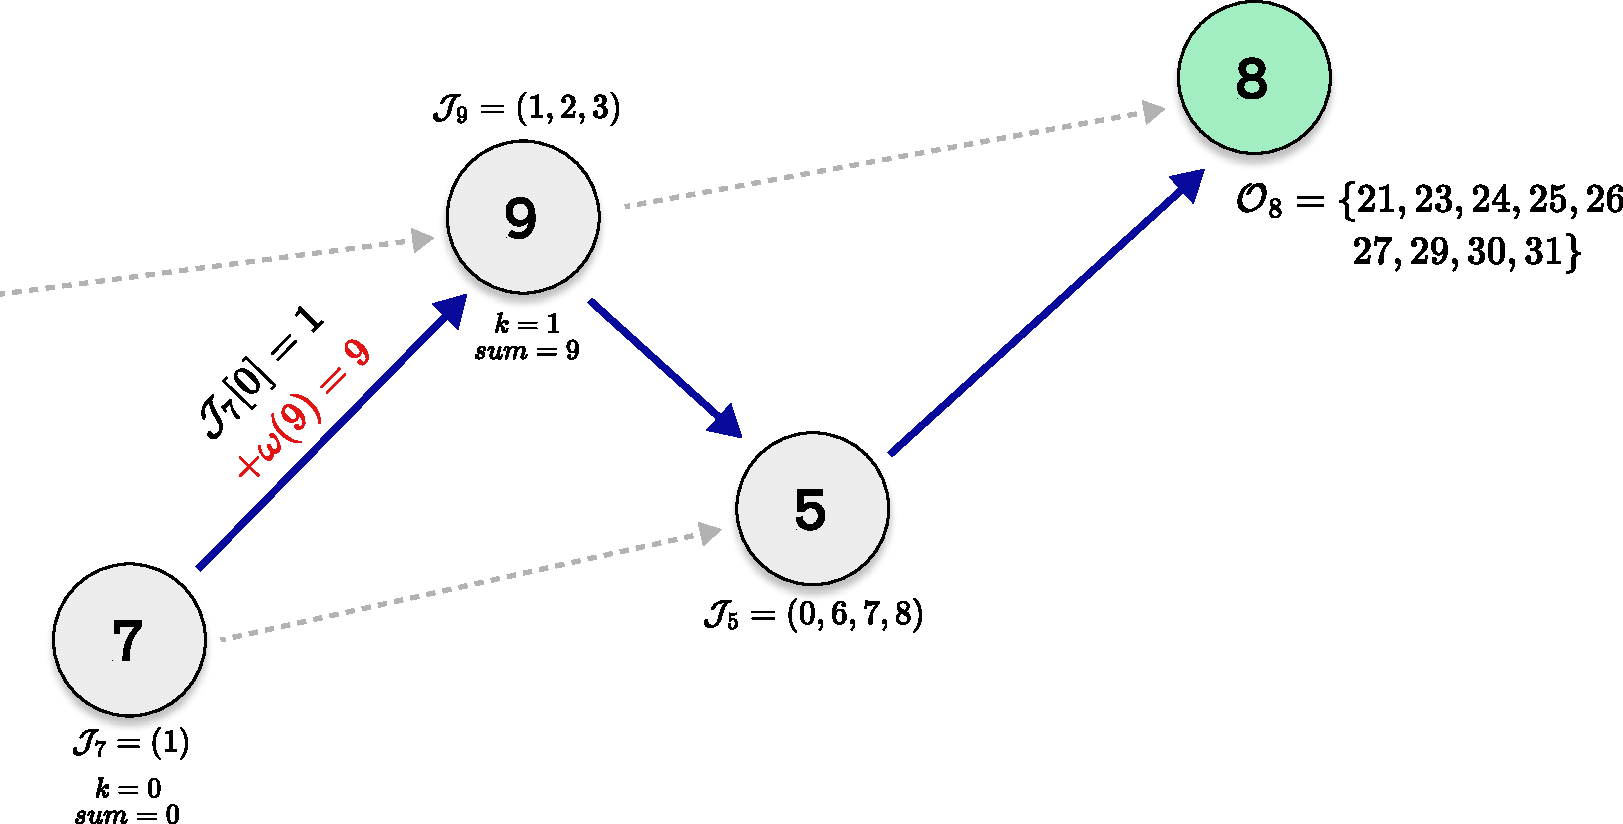
\includegraphics[width=0.9\textwidth]{assets/dag_query2.pdf}}
        \only<3>{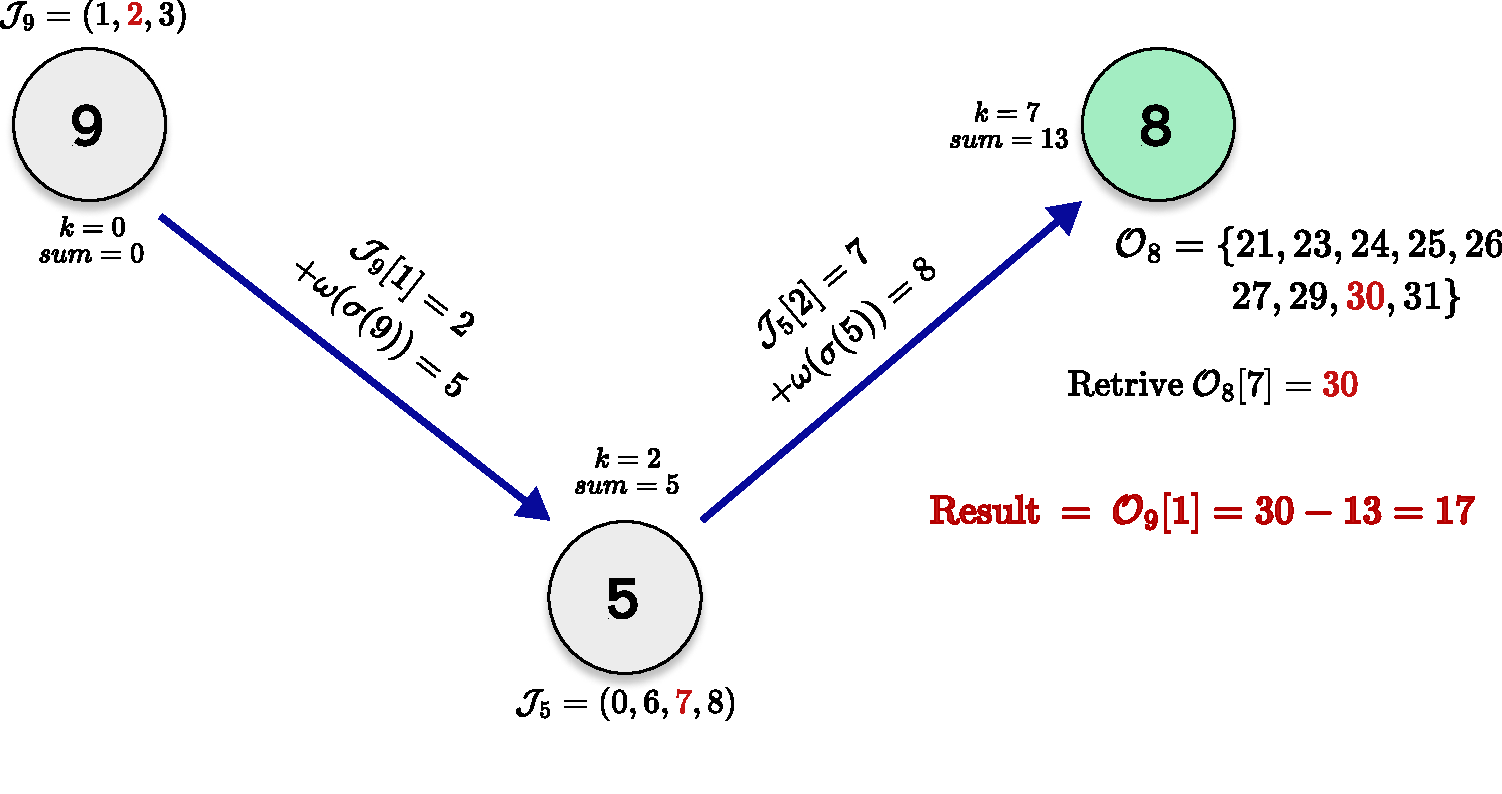
\includegraphics[width=0.9\textwidth]{assets/dag_query3.pdf}}
        % \only<4>{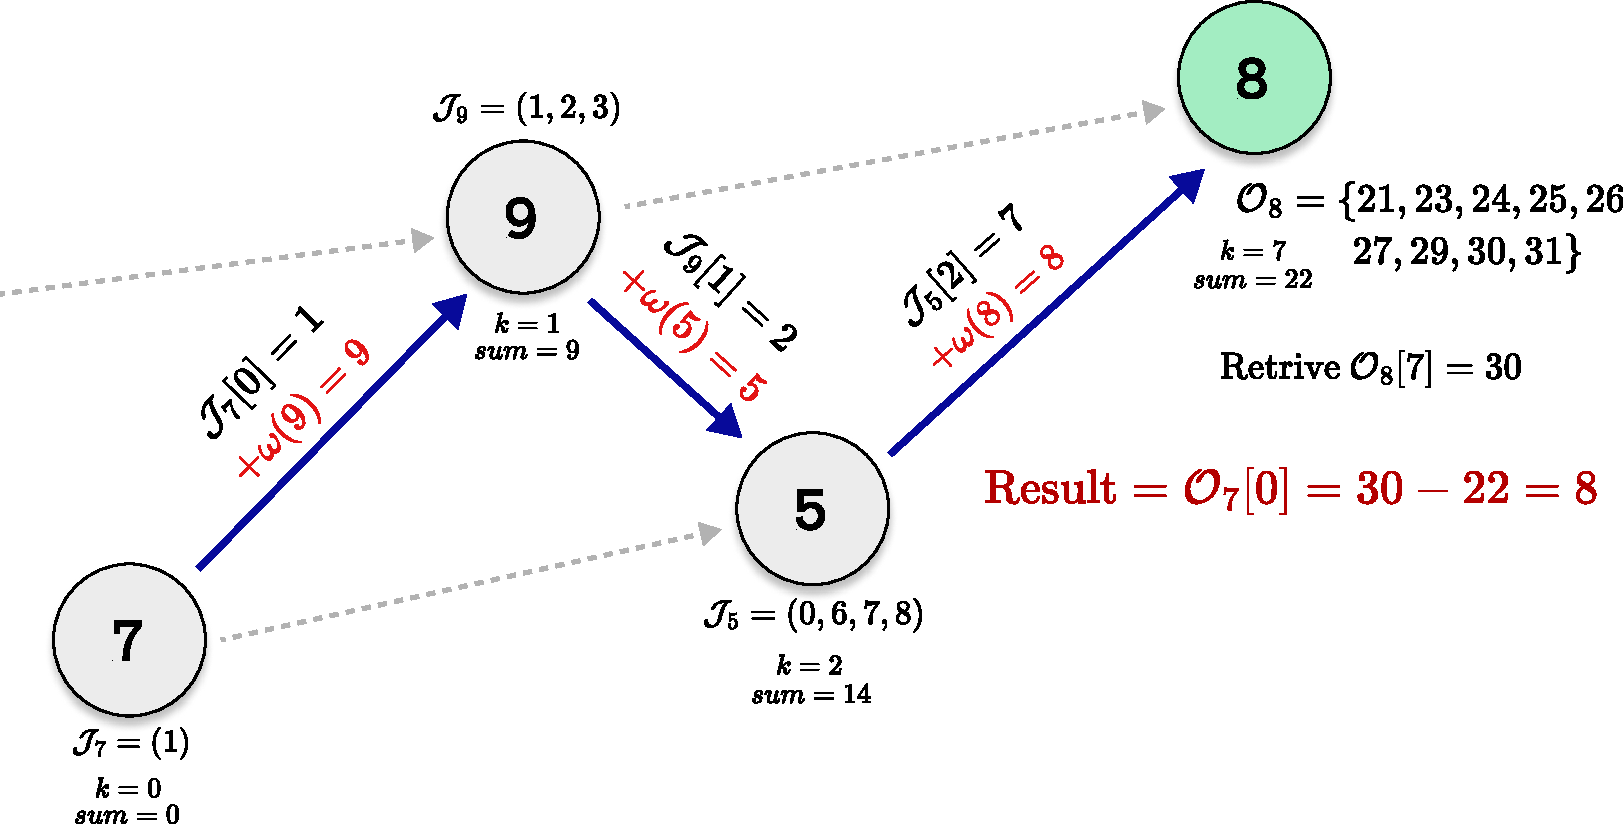
\includegraphics[width=0.9\textwidth]{assets/dag_query4.pdf}}
    \end{figure}
\end{frame}

% --- SLIDE 18: Example: Computing O_7[0] (Dynamic Structure) ---
\begin{frame}{Succinct Data Structure: Components}
    \framesubtitle{Arrays Indexed by Vertex ID}
    % divide in two columns
    \begin{columns}[T]
        \column{0.5\textwidth}
        \uncover<1->{\begin{center}
                \textbf{Each node stores 3 components}
            \end{center}
            \begin{center}
                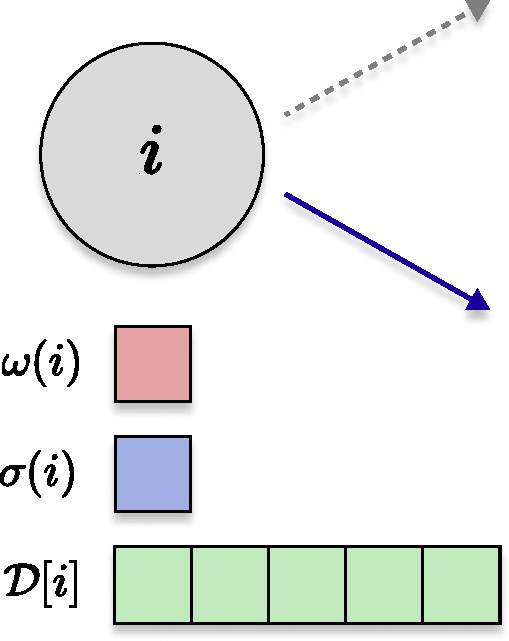
\includegraphics[width=0.55\textwidth]{assets/AoS.pdf}
            \end{center}}

        \column{0.5\textwidth}
        \uncover<2->{\begin{center}
                \textbf{Succinct DAG as a Struct of Arrays}
            \end{center}
            \begin{center}
                \vspace{0.5em}
                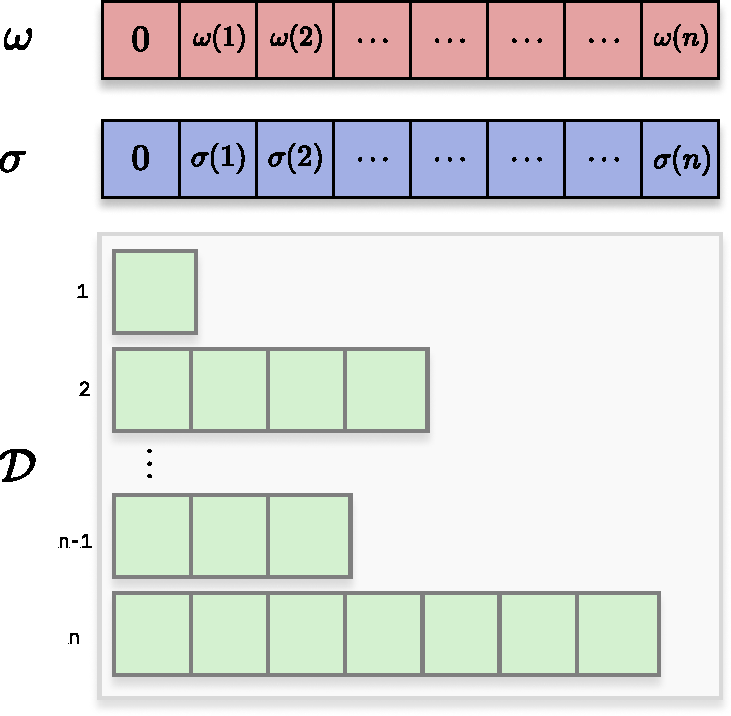
\includegraphics[width=0.8\textwidth]{assets/SoA.pdf}
            \end{center}}
    \end{columns}
\end{frame}


% \subsection{Querying}
% % --- SLIDE 26: Reconstructing O-Set Elements: The Idea ---
% \begin{frame}{Reconstructing $\mathcal{O}$-Set Elements}
%     \framesubtitle{Finding $\mathcal{O}_v[k]$ for Implicit Nodes}

%     \begin{alertblock}{How?}
%         Follow the designated successor path $\sigma(v) \to \sigma(\sigma(v)) \to \dots \to e$ until an explicit node $e$ is reached.
%     \end{alertblock}


%     \begin{itemize}
%         \item Use the stored offset sequences $\mathcal{I}$ to find the corresponding index at each step.
%         \item Accumulate the weights $w(\cdot)$ along the path.
%         \item Retrieve the value from the explicit node's $\mathcal{O}_e$ and subtract the accumulated weight.
%     \end{itemize}

%     \vspace{3ex}
%     \pause
%     Let's see an example for $\mathcal{O}_7[0]$

% \end{frame}


% % --- SLIDE 28: Computing the Rank Query (RankG) (Columns Layout) ---
% \begin{frame}{Computing the Rank Query for a Node $N$}
%     \framesubtitle{High-Level Steps}

%     \begin{columns}[c] % T aligns tops
%         % Colonna sinistra: Diagramma di flusso
%         \begin{column}{0.65\textwidth}
%             \centering % Center the diagram within the column
%             \begin{tikzpicture}[node distance=1cm, auto, >=latex,
%                     box/.style={rectangle, draw, thick, text centered, minimum height=2em, minimum width=4.5cm, font=\sffamily}, % Slightly wider boxes
%                     arrow/.style={->, thick}]

%                 % Overlay on nodes to make them appear one by one
%                 \node<1-> [box] (step1) {1. Compute $\mathcal{O}_N$};
%                 \node<2-> [box, below=of step1] (step2) {2. Generate Intervals $I_x$};
%                 \node<3-> [box, below=of step2] (step3) {3. Sort Intervals};
%                 \node<4-> [box, below=of step3] (step4) {4. Merge Intervals};
%                 % Result node appears with the last arrow
%                 \node<5-> [right=1.5cm of step4] (result) {\alert{$\textsf{rank}_G(N)$}};

%                 % Overlay on arrows to match the next step appearing
%                 \draw<2-> [arrow] (step1) -- (step2);
%                 \draw<3-> [arrow] (step2) -- (step3);
%                 \draw<4-> [arrow] (step3) -- (step4);
%                 \draw<5-> [arrow] (step4) -- (result);
%             \end{tikzpicture}
%         \end{column}

%         % Colonna destra: Reminder
%         \begin{column}{0.35\textwidth}
%             \uncover<2->{ % This block appears at step 4
%                 \begin{alertblock}{Reminder}
%                     Intervals are
%                     $$I_x = [\max(0, x - w(N) + 1), x]$$
%                 \end{alertblock}
%             }
%         \end{column}
%     \end{columns}

% \end{frame}


% \subsection{Compression}
\section{Compression Strategies}
\label{sec:compression_strategies}

The succinct representation presented in \autoref{sec:succinct_dag_representation} consists of arrays for weights ($\mathcal{W}$), successor information ($\Sigma$), and associated data ($\mathcal{D}$). To further reduce the memory footprint beyond the gains achieved by the explicit/implicit node partitioning, this section discusses compression techniques for each component.

We primarily consider variable-length integer coding (\autoref{sec:integer_coding}), Elias-Fano encoding (\autoref{sec:elias_fano_code}), and Run-Length Encoding (RLE), aiming to preserve efficient access needed for query evaluation (Algorithms~\ref{alg:get_value} and \ref{alg:rank_dag}), potentially using structures like the compressed integer vectors from \autoref{app:compressed_intvec_engineering}.

\subsection{Weights and Successors}
\label{subsec:compressing_W_Sigma}

The components $\mathcal{W}$ and $\Sigma$ are arrays of integers, both without any guarantee of monotonicity or specific distribution patterns a priori.
\begin{itemize}
    \item $\mathcal{W}$: An array of length $n = |V|$, where $\mathcal{W}[v] = w(v) \in \mathbb{N}_0$. The values are non-negative integers representing vertex weights.
    \item $\Sigma$: An array of length $n$, where $\Sigma[v]$ stores either the integer ID $\sigma(v) \in \{0, \dots, n-1\}$ if $v \in V_I$, or a special marker (which can also be represented as an integer) if $v \in V_E$.
\end{itemize}

% Given that both $\mathcal{W}$ and $\Sigma$ are sequences of integers, the variable-length integer coding schemes discussed in \autoref{sec:integer_coding} are natural candidates for compression. Techniques such as Unary, Elias Gamma/Delta, or Rice codes can be employed. The optimal choice depends heavily on the empirical distribution of the weights $w(v)$ and the successor IDs $\sigma(v)$ (and the chosen marker value) within the specific DAG instance.

% A practical approach to implement this compression while preserving the necessary random access capability (i.e., efficiently retrieving $\mathcal{W}[v]$ or $\Sigma[v]$ for any $v$) is provided by the engineered \textsf{compressed-intvec} structure described in \autoref{app:compressed_intvec_engineering}. This structure allows selecting an appropriate integer codec (e.g., Gamma, Delta, Rice) based on the data distribution and employs a sampling mechanism to ensure $O(1)$ expected time access to any element $v$, at the cost of a typically sub-linear space overhead for the samples.

% Alternatively, if the range of possible integer values in $\mathcal{W}$ or $\Sigma$ (i.e., the maximum weight or $n$) is sufficiently small to be considered a small alphabet $\alpha$, one could choose to use Wavelet Trees (\autoref{sec:wavelet_trees}), particularly efficient variants like Wavelet Matrices or Quad Wavelet Trees (\autoref{sec:wavelet_matrices_and_quad_vectors}). These structures provide efficient Access (retrieving the element at a given position) in $O(\log \alpha)$ time, where $\alpha$ is the size of the alphabet (the number of distinct values). However, for general graphs where weights or vertex counts $n$ can be large, the alphabet size may not be small, making direct integer coding via \textsf{compressed-intvec} a more generally applicable starting point.

Since both $\mathcal{W}$ and $\Sigma$ are integer sequences, variable-length coding schemes from \autoref{sec:integer_coding} (e.g., Unary, Elias Gamma/Delta, Rice codes) are applicable. The choice of the best code depends on the observed distribution of weights and successor IDs.

To combine compression with efficient random access (retrieving $\mathcal{W}[v]$ or $\Sigma[v]$), the \textsf{compressed-intvec} structure (\autoref{app:compressed_intvec_engineering}) is a suitable implementation choice. It allows selecting an appropriate integer codec and uses sampling to achieve constant expected time access, with sub-linear space overhead for samples.

Alternatively, if the range of values (maximum weight or $n$) is small, treating them as symbols from a small alphabet $\alpha$ allows using Wavelet Trees (\autoref{sec:wavelet_trees}) or related structures (\autoref{sec:wavelet_matrices_and_quad_vectors}). These offer $O(\log |\alpha|)$ access time. However, for general graphs with potentially large weights or vertex counts, direct integer coding via \textsf{compressed-intvec} is often more practical.

\subsection{Associated Data Sequences}
\label{subsec:compressing_associated_data_sequences}

The associated data component $\mathcal{D}$ stores sequences that encode path weight information. Specifically, for an explicit vertex $v \in V_E$, $\mathcal{D}[v]$ holds the $\mathcal{O}$-set $\mathcal{O}_v = (x_0, \dots, x_{m-1})$, and for an implicit vertex $v \in V_I$, it holds the offset sequence $\mathcal{I}_v = (j_0, \dots, j_{m-1})$. Both $\mathcal{O}_v$ and $\mathcal{I}_v$ are sequences of non-negative integers which are strictly increasing ($x_k < x_{k+1}$ and $j_k < j_{k+1}$ respectively), as established by their definitions and construction rules.

This strictly monotonic property makes these sequences suitable for specialized compression techniques. Elias-Fano encoding (\autoref{sec:elias_fano_code}), discussed previously, is a strong candidate offering both good compression ratios and efficient support for operations like random access. An alternative approach, particularly effective when sequences contain long stretches of consecutive integers, is Run-Length Encoding (RLE). We detail the RLE representation below.

\subsubsection*{Run-Length Encoding (RLE) Representation}
Run-Length Encoding compresses a monotonic sequence by identifying and representing consecutive values efficiently. Consider a generic strictly increasing sequence $Y = (y_0, y_1, \dots, y_{m-1})$. A \emph{run} is a maximal contiguous subsequence $(y_i, y_{i+1}, \dots, y_{i+l-1})$ where each element is exactly one greater than its predecessor ($y_{j+1} = y_j + 1$ for $i \le j < i+l-1$). A run can have length $l=1$. RLE represents the sequence $Y$ by encoding each run using its starting value and its length.

The RLE process generates two auxiliary sequences:
\begin{itemize}
    \item The \emph{run starts sequence}, $S = (s_1, s_2, \dots, s_p)$, contains the first value $s_i$ of the $i$-th run in $Y$. Since runs are maximal and $Y$ is strictly increasing, $S$ is also strictly increasing.
    \item The \emph{run lengths sequence}, $L = (l_1, l_2, \dots, l_p)$, contains the length $l_i \ge 1$ of the $i$-th run. $L$ is a sequence of positive integers with no other guaranteed properties.
\end{itemize}
The pair $(S, L)$ allows for the exact reconstruction of $Y$. Algorithm \ref{alg:rle_encode} outlines the procedure to compute $S$ and $L$ from $Y$.

\begin{algorithm}[htbp]
    \caption{$\textsc{EncodeRLE}(Y)$: RLE encoding of a monotonic sequence}
    \label{alg:rle_encode}
    \small
    \begin{algorithmic}[1]
        \Require Monotonic sequence $Y = (y_0, y_1, \dots, y_{m-1})$, where $m = |Y|$.
        \Ensure Run starts sequence $S$, Run lengths sequence $L$.
        \State Initialize $S \leftarrow \emptyset$, $L \leftarrow \emptyset$.
        \If{$m = 0$}
        \State \Return $(S, L)$
        \EndIf
        \State $i \leftarrow 0$
        \While{$i < m$}
        \State $current\_start \leftarrow y_i$
        \State $current\_length \leftarrow 1$
        \While{$i + 1 < m$ and $y_{i+1} = y_i + 1$}
        \State $current\_length \leftarrow current\_length + 1$
        \State $i \leftarrow i + 1$
        \EndWhile
        \State Append $current\_start$ to $S$.
        \State Append $current\_length$ to $L$.
        \State $i \leftarrow i + 1$
        \EndWhile
        \State \Return $(S, L)$
    \end{algorithmic}
\end{algorithm}

The space efficiency of RLE relies on effectively compressing the resulting sequences $S$ and $L$.
The run starts sequence $S = (s_1, \dots, s_p)$ is strictly monotonic. Consequently, it is an ideal candidate for Elias-Fano encoding (\autoref{sec:elias_fano_code}).

The run lengths sequence $L = (l_1, \dots, l_p)$ is a sequence of positive integers without guaranteed structure. Standard variable-length integer codes (\autoref{sec:integer_coding}), such as Elias Gamma or Delta codes, can be applied. In practice, employing a structure like the \textsf{compressed-intvec} (\autoref{app:compressed_intvec_engineering}) allows choosing an appropriate codec and provides efficient random access.

\subsubsection*{Random Access with RLE Sequences}
Retrieving the element $y_k$ (the element at index $k$ in the original sequence $Y$, $0 \le k < m$) from the RLE representation $(S, L)$ requires identifying the run to which $y_k$ belongs. This necessitates finding the unique run index $i^*$ (where $1 \le i^* \le p$) such that:
\[ \sum_{j=1}^{i^*-1} l_j \le k < \sum_{j=1}^{i^*} l_j \]
where the sum is defined as $0$ if $i^*=1$. Once $i^*$ is found, the value $y_k$ is given by:
\[ y_k = s_{i^*} + \left( k - \sum_{j=1}^{i^*-1} l_j \right) \]
Computing the prefix sums $\sum l_j$ on the fly requires iterating through $L$, potentially leading to $O(p)$ time complexity for access, which is inefficient if the number of runs $p$ is large.

To accelerate random access, one can precompute and store the sequence of prefix sums of the run lengths:
\[ P = (p_1, p_2, \dots, p_p) \qquad  p_i = \sum_{j=1}^{i} l_j. \]
Since $l_j \ge 1$ for all $j$, the sequence $P$ is strictly increasing. As a strictly monotonic sequence, $P$ itself can be compressed effectively, for instance, using Elias-Fano encoding.

With the prefix sum sequence $P$ available, finding the index $i^*$ corresponding to the query index $k$ reduces to searching for the smallest $i^*$ such that $p_{i^*} > k$. This is a successor search problem on the monotonic sequence $P$. Using binary search on $P$ (if stored as an array) takes $O(\log p)$ time. If $P$ is stored in a structure supporting faster searches (like rank/select structures built upon certain Elias-Fano constructions), this lookup time might be further improved. Algorithm \ref{alg:rle_get_value} formalizes access using prefix sums.

\begin{algorithm}[htbp]
    \caption{$\textsc{GetValueRLE}(S, L, P, k)$: Retrieve element from RLE} % Renamed for clarity
    \label{alg:rle_get_value}
    \small
    \begin{algorithmic}[1]
        \Require $S=(s_1,\dots,s_p)$, $L=(l_1,\dots,l_p)$, $P=(p_1, \dots, p_p)$, $k \in [0, m-1]$.
        \Ensure The value $y_k$ of the element at index $k$.
        \State Find smallest $i^* \in \{1, \dots, p\}$ such that $P[i^*] > k$.
        \If{$i^* = 1$}
        \State $previous\_cumulative\_length \leftarrow 0$
        \Else
        \State $previous\_cumulative\_length \leftarrow P[i^*-1]$
        \EndIf
        \State $offset \leftarrow k - previous\_cumulative\_length$
        \State $start\_value \leftarrow S[i^*]$
        \State \Return $start\_value + offset$
    \end{algorithmic}
\end{algorithm}

\subsubsection*{Choosing Between Elias-Fano and RLE}
The choice between direct Elias-Fano encoding and Run-Length Encoding (RLE) for representing the strictly increasing sequences $\mathcal{O}_v$ and $\mathcal{I}_v$ depends on their structure. RLE is advantageous when the sequence exhibits significant clustering, meaning the number of runs $p$ is substantially smaller than the total number of elements $m$ ($p \ll m$). In such cases, the combined compressed size of the run starts $S$ and run lengths $L$ (and potentially the prefix sums $P$) might be less than direct Elias-Fano encoding of the original sequence.

On the other hand, if sequences are sparse or lack significant runs ($p$ is close to $m$), direct Elias-Fano is likely more straightforward and potentially more space-efficient.

Regardless of the chosen compression method, representing the entire associated data component $\mathcal{D}$ practically involves concatenating the compressed representations of all sequences ($\{\mathcal{D}_E(v)\}_{v \in V_E}$ and $\{\mathcal{D}_I(v)\}_{v \in V_I}$) into a single buffer. An auxiliary index structure is then needed to map each vertex ID $v$ to the starting position and metadata of its compressed sequence. The space overhead for this index is typically negligible compared to the compressed data itself


% \subsection{Achieving Sub-Entropy Space for Path Queries}
% --- SLIDE 20: Baseline: Graph Entropy H0(G) ---
\begin{frame}{Space Efficiency: Baseline Comparison}
    \framesubtitle{How Much Information is in the Graph?}
    To evaluate our structure's space, \alert{we need a baseline}.
    \begin{block}<1->{$0^{th}$-Order Graph Entropy $H_0(G)$}
        A theoretical lower bound for storing the \emph{entire} weighted DAG ($V, E, w$) losslessly.
        \[ H_0(G) = \underbrace{H_W(G)}_{\text{Cost for Weights}} + \underbrace{H_E(G)}_{\text{Cost for Topology (Edges)}} \]
    \end{block}
    \begin{itemize}
        \item<2-> $H_W(G) \approx \sum_{v \in V} \log(w(v)+1)$ bits (\emph{Minimal binary encoding for weights}).
        \item<3-> $H_E(G) \approx \log \binom{n(n-1)}{m}$ bits (\emph{Cost to choose $m=|E|$ edges out of all possible $n(n-1)$}).
    \end{itemize}
    \vspace{0.5em}
    \uncover<4->{\textbf{Any method saving the \emph{full} graph structure needs at least $H_0(G)$ bits!}}

\end{frame}


% --- SLIDE 21: Space Comparison - Key Numbers ---
\begin{frame}{Space Comparison: Succinct Structure vs. Baselines}
    \framesubtitle{Bitcoin DAG Example ($n \approx 22k, m \approx 50k$)}
    \begin{columns}[c] % Keep [t] for top alignment
        \begin{column}{0.5\textwidth} % Adjusted width potentially
            \centering
            \begin{tabular}{l r}
                \toprule
                \textbf{Method}                       & \textbf{Estimated Bits}          \\
                \midrule
                \textbf{Theoretical Lower Bound}      & \uncover<1->{\textbf{1,525,730}} \\
                \quad Weights $H_W(G)$                & \uncover<1->{60,824}             \\
                \quad Topology $H_E(G)$               & \uncover<1->{1,464,906}          \\
                \midrule
                \textit{Precomputed Rank Queries:}    &                                  \\
                \quad Explicit Binary Storage         & \uncover<2->{4,854,533}          \\
                \quad Elias-Fano Compressed           & \uncover<2->{2,211,849}          \\
                \midrule
                \textbf{Our Succinct DAG}             & \uncover<3->{\textbf{602,808}}   \\
                \quad Weights $\mathcal{W}$           & \uncover<3->{60,824}             \\
                \quad Successors $\Sigma$             & \uncover<3->{297,700}            \\
                \quad Assoc. Data $\mathcal{D}$ (RLE) & \uncover<3->{244,284}            \\
                \bottomrule
            \end{tabular}
            % Removed \end{center}
        \end{column}
        \begin{column}{0.5\textwidth} % Adjusted width to sum to 1.0
            % \begin{alertblock}<4->{Key Result}
            %     Our structure ($S(G)$) is $\approx$ \textbf{2.5x smaller} than the theoretical lower bound ($H_0(G)$) and $\approx$ \textbf{3.7x smaller} than compressed precomputation.
            % \end{alertblock}
            \begin{alertblock}<4->{Achieving Sub-Entropy Space: How?}
                Our structure is \textbf{lossy} regarding the full graph topology:
                \begin{itemize}
                    \item It \alert{does not store} the complete edge set.
                    \item It only stores the chosen successor $\sigma(v)$ for each implicit node (in $\Sigma$).
                \end{itemize}
                However, it is \textbf{lossless} for computing the specific \alert{Rank Query}.
            \end{alertblock}
        \end{column}
    \end{columns}
\end{frame}


% % --- SLIDE 22: Achieving Sub-Entropy Space: Why? (Corrected TikZ) ---
% \begin{frame}{Achieving Sub-Entropy Space: How is it Possible?}
%     \framesubtitle{Targeted Information Retention}

%     Why can our structure $S(G)$ use less space than the graph entropy $H_0(G)$?


%     \begin{center}
%         \begin{tikzpicture}[node distance=1cm, auto, >=latex,
%                 box/.style={rectangle, draw, thick, text centered, minimum height=3em, font=\sffamily, minimum width=5.5cm, align=center}, % Adjusted size and added align
%                 arrow/.style={->, thick}]

%             % Left Box: H0(G) stores the full Edge set E
%             \node [box, fill=red!10] (H0) {$H_0(G)$: Encodes \\ Full Graph $(V, \mathbf{E}, w)$};

%             % Right Box: S(G) stores only Successor info Sigma
%             \node [box, fill=green!10, right=2cm of H0] (SG) {$S(G)$: Encodes \\ $(\mathcal{W}, \Sigma, \mathcal{D})$};

%             % Labels above boxes
%             \node [above=0.3cm of H0, text width=5.5cm, align=center] {\small \textbf{Lossless Graph Encoding}};
%             \node [above=0.3cm of SG, text width=5.5cm, align=center] {\small \textbf{Our Succinct Structure}};

%         \end{tikzpicture}
%     \end{center}

%     \begin{alertblock}<1->{The Reason: Lossy Topology}
%         Our structure is \textbf{lossy} regarding the full graph topology:
%         \begin{itemize}
%             \item It \alert{does not store} the complete edge set $E$.
%             \item It only stores the chosen successor $\sigma(v)$ for each implicit node (in $\Sigma$).
%         \end{itemize}
%         However, it is \textbf{lossless} for computing the specific \alert{Rank Query}.
%     \end{alertblock}
%     % \uncover<2->{It retains only the information necessary for the target query, discarding unused topological details.}
% \end{frame}


% \section{Conclusion and Next Steps}
\chapter{Conclusion and Future Directions}
\label{chap:conclusion}

This thesis began by covering data compression, succinct data structures and sequence queries. Building on that foundation, Chapter \ref{chap:succinct_dags} introduced our primary contribution: a space-efficient method for representing node-weighted Directed Acyclic Graphs (DAGs). This representation is specifically designed to support \Rank{} (\ref{def:rank_dag}) queries, which aggregate cumulative path weights ending at a particular vertex.

The core contribution presented in Chapter \ref{chap:succinct_dags} is a succinct representation strategy for weighted DAGs. Motivated initially by the reinterpretation of the degenerate string problem as a graph problem, we generalized the approach to arbitrary weighted DAGs. The key idea involves partitioning the vertices into two sets: explicit vertices ($V_E$), typically comprising the sink nodes, for which path weight information ($\mathcal{O}$-sets) is stored directly; and implicit vertices ($V_I$), for which this information is derived indirectly. This derivation relies on a carefully defined successor function, $\sigma$, which designates a specific successor for each implicit node, guiding a traversal path. Associated with each implicit node $v$, an offset sequence $\mathcal{I}_v$ stores the necessary indices to reconstruct its $\mathcal{O}$-set elements from the $\mathcal{O}$-set of its designated successor $\sigma(v)$. Query algorithms, notably \textsc{GetValue} (\ref{alg:get_value}) and \textsc{GetOSet} (\ref{alg:get_o_set}), were presented, demonstrating how to reconstruct the path weight information by traversing these successor paths until an explicit node is reached.

Furthermore, we investigated compression strategies for the components of our structure,vertex weights $\mathcal{W}$, successor information $\Sigma$, and the associated data $\mathcal{D}$ (containing $\mathcal{O}$-sets or $\mathcal{I}$ sequences). Techniques such as variable-length integer coding and Run-Length Encoding, coupled with methods like Elias-Fano encoding for monotonic sequences, were discussed to minimize space occupancy. A significant finding highlighted in Section \ref{sec:below_entropy} is that the space usage of our proposed structure can fall below the established $0^{th}$-order entropy lower bound for lossless graph representation. This is possible because our structure is tailored specifically for the \Rank{} query and does not retain the full topological information (the complete edge set $E$) of the original DAG, thereby achieving high space efficiency for its designated task compared to both lossless graph encodings and methods based on precomputing query results.

While the developed succinct DAG representation offers substantial space savings, a potential performance consideration arises from the query evaluation process itself. The time required to compute a query for an implicit node $v$ depends directly on the length of the successor path that must be traversed from $v$ until an explicit node is encountered (as seen in Algorithm \ref{alg:get_value}). In large or deep DAGs, these paths could potentially become long, leading to variability and potentially slow query times in the worst case for certain nodes. This observation motivates a primary direction for future research: enhancing the query time predictability and efficiency by ensuring that all implicit nodes are reasonably close to an explicit node within the successor path structure.

To address this, instead of relying solely on the sink nodes as the base cases for path traversal, we propose a strategy based on ensuring a maximum traversal distance, denoted by a predefined integer $k$. The core idea is to augment the original set of explicit nodes $V_E$ (initially, the sinks) with a carefully selected subset of currently implicit nodes, resulting in a new, larger set of explicit nodes $V'_E \supseteq V_E$. This target set $V'_E$ must satisfy a specific property related to the successor function $\sigma$: every vertex $v$ that remains implicit (i.e., $v \in V \setminus V'_E$) must be able to reach some node $u \in V'_E$ by following the successor path defined by $\sigma$, using at most $k$ steps. More formally, let the successor path starting from $v$ be the sequence $v_0=v, v_1=\sigma(v_0), v_2=\sigma(v_1), \dots$. Then, for every $v \in V \setminus V'_E$, there must exist an index $j$, where $0 \le j \le k$, such that $v_j \in V'_E$.

The challenge then becomes selecting such a set $V'_E$ that is as small as possible, in order to minimize the additional space overhead associated with storing the $\mathcal{O}$-sets explicitly for these newly designated explicit nodes. This optimization problem is conceptually analogous to finding a minimum distance-$k$ dominating set in a graph. In the standard definition, a distance-$k$ dominating set $D$ is a subset of vertices such that every vertex not in $D$ is within a distance of $k$ (measured by the number of edges in a shortest path) from at least one vertex in $D$. Our formulation adapts this concept: the distance is measured specifically along the directed paths induced by the successor function $\sigma$, and the goal is to find a set $V'_E$ of minimum cardinality that \emph{dominates} all other vertices within $k$ steps along these $\sigma$-paths. Finding a minimum distance-$k$ dominating set is known to be an NP-hard problem for general graphs \cite{haynes2013fundamentals}. Furthermore, the problem of finding a minimum cardinality set $V'_E$ satisfying our $k$-step $\sigma$-path constraint on a DAG is also NP-hard; this can be demonstrated through a reduction from the Set Cover problem, indicating that finding an optimal solution is likely computationally intractable for large DAGs.

Consequently, a practical direction for future investigation involves the design and analysis of efficient heuristics. Such heuristics would aim to construct a set $V'_E$ satisfying the $k$-distance requirement along $\sigma$-paths, while keeping its size reasonably small, even if not guaranteeing absolute minimality. The choice of heuristic would need to balance the quality of the solution (size of $V'_E$) with the computational cost of finding it.

Once a suitable set $V'_E$ has been determined (whether optimally or via a heuristic), the successor selection function $\sigma$ needs to be redefined to leverage this structure. For an implicit node $v \in V \setminus V'_E$, the choice of its designated successor $\sigma(v)$ from the set $Succ(v)$ should prioritize reaching \emph{any} node within the target set $V'_E$ as quickly as possible along the subsequent $\sigma$-path. That is, $\sigma(v)$ should ideally be selected as the node $u \in Succ(v)$ which minimizes the length of the $\sigma$-path starting from $u$ to the nearest node in $V'_E$. Ties in path length could be resolved using secondary criteria, such as minimizing the $\mathcal{O}$-set cardinality $|\mathcal{O}_u|$ (as in the original heuristic) or simply selecting the successor with the minimum vertex identifier.

Implementing this refined strategy directly imposes an upper bound of $k$ on the number of iterations performed by the main loop in Algorithm \ref{alg:get_value}. This provides a worst-case guarantee on the time complexity of the path traversal component for any \Rank{} query, making the overall query performance significantly more predictable and uniform across all nodes, regardless of their position within the DAG. The main trade-off shifts to the selection of the parameter $k$: smaller values of $k$ yield faster worst-case query times but likely necessitate larger (and thus more space-consuming) sets $V'_E$, whereas larger values of $k$ may permit smaller sets $V'_E$ at the expense of a higher query time bound.

\backmatter

% QUESTIONS?
\begin{frame}[noframenumbering]{Worst-Case $\mathcal{O}$-Set Size: Is Exponential Growth Possible?}
    \framesubtitle{Understanding the $\mathcal{O}$-set Size}

    \begin{block}{Exponential Growth Can Occur}
        The cardinality of an $\mathcal{O}$-set, $|\mathcal{O}_v|$, is not generally bounded by a polynomial in the number of vertices $|V|$. It can grow exponentially.
    \end{block}

    \begin{block}{Underlying Reason: Path Count}
        The number of distinct paths from a source $s$ to a vertex $v$, denoted $|Path(s, v)|$, can itself be exponential in certain DAG structures. Since $|\mathcal{O}_v| \le |Path(s, v)|$, the potential for exponential size exists.
    \end{block}

    \pause % Optional pause

    \begin{alertblock}{Key Condition for Exponential Growth}
        The exponential potential is realized if the vertex weights $w(v)$ are assigned such that distinct paths $P_1 \neq P_2$ almost always lead to distinct cumulative weights $W(P_1) \neq W(P_2)$.
    \end{alertblock}

\end{frame}

\begin{frame}[noframenumbering]{Achieving Exponential $\mathcal{O}$-Set Size}
    \framesubtitle{A Strategy for Path Weight Uniqueness}

    Start with a DAG structure that naturally admits an exponential number of paths between two nodes. An example is a layered graph with multiple choices at each layer transition.

    \begin{alertblock}{Strategic Weight Assignment}
        Assign vertex weights $w(v)$ carefully to ensure path weight uniqueness.
        \[ w(v) = 2^k \quad \text{(using a unique exponent } k \text{ for each node)} \]
    \end{alertblock}

    \pause

    \begin{block}{Mechanism: Unique Binary Representation}
        With power-of-2 weights, the cumulative path weight $W(P) = \sum_{v \in P \setminus \{s\}} w(v)$ becomes a sum of distinct powers of 2.
        Due to the uniqueness of binary representation, different sets of nodes (i.e., different paths) produce different sums.
        Therefore, $|Path(s, v)|$ distinct paths yield $|\mathcal{O}_v| = |Path(s, v)|$ distinct weights.
    \end{block}

\end{frame}

\end{document}
